%%%%%%%%%%%%%%%%%%%%%%%%%%%%%%%%%%%%%%%%%
% Główny plik pracy
% Szablon pracy dyplomowej
% Wydział Informatyki 
% Zachodniopomorski Uniwersytet Technologiczny w Szczecinie
% autor Joanna Kołodziejczyk (jkolodziejczyk@zut.edu.pl)
% Bardzo wczesnym pierwowzorem szablonu był
% The Legrand Orange Book
% Version 5.0 (29/05/2025)
%
% Modifications to LOB assigned by %JK
%%%%%%%%%%%%%%%%%%%%%%%%%%%%%%%%%%%%%%%%%


%----------------------------------------------------------------------------------------
%	PAKIETY ORAZ PLIKI ZAWIERAJĄCE DEFINICJE STYLI I KONFIGURACJĘ OTOCZEŃ LATEX
%----------------------------------------------------------------------------------------
\documentclass[12pt,fleqn,twoside]{book} % JK Rozmiary czcionek są zgodne z wymaganiami uczelni 
% UWAGA! - wydruk jest dwustronny i jest to zabieg zamierzony
% (removed duplicate) biblatex is loaded in structure.tex
\usepackage{graphicx} 
\usepackage{float} 
\usepackage{plantuml} 
\usepackage{listings}          % do wyświetlania kodu
\lstset{                       % ustawienia dla listings
  basicstyle=\ttfamily\small,
  language=Java,
  frame=single,
  breaklines=true
}
\usepackage[utf8]{inputenc}   % kodowanie UTF-8
\usepackage[T1]{fontenc}      % poprawne łamanie słów, polskie znaki
\usepackage[polish]{babel} 
% \usepackage{fix-cm} % Zapewnienie, że wszystkie rozmiary czcionek są dostępne

%%%%%%%%%%%%%%%%%%%%%%%%%%%%%%%%%%%%%%%%%
% Plik konfigurujący
% Szablon pracy dyplomowej
% Wydział Informatyki 
% Zachodniopomorski Uniwersytet Technologiczny w Szczecinie
% autor Joanna Kołodziejczyk (jkolodziejczyk@zut.edu.pl)
% Bardzo wczesnym pierwowzorem szablonu był
% The Legrand Orange Book
% Version 5.0 (29/05/2025)
%
% Modifications to LOB assigned by %JK
%%%%%%%%%%%%%%%%%%%%%%%%%%%%%%%%%%%%%%%%%


%----------------------------------------------------------------------------------------
%	VARIOUS REQUIRED PACKAGES AND CONFIGURATIONS
%----------------------------------------------------------------------------------------

%GEOMETRY
\usepackage[top=3.2cm,bottom=3.5cm,left=2.5cm,right=2.5cm,headsep=1.5ex,bindingoffset=1cm,a4paper]{geometry} % Page margins

% GRAPHICS
\usepackage{graphicx} % Required for including pictures
\graphicspath{{Pictures/}} % Specifies the directory where pictures are stored

% For math equations, theorems, symbols, etc
\usepackage{amsmath,amsfonts,amssymb,amsthm} 
\usepackage[section]{placeins}
% Customize lists
\usepackage{enumitem} 
\setlist{nolistsep} % Reduce spacing between bullet points and numbered lists
\setlist[itemize]{label=--}

% Required for nicer horizontal rules in tables
\usepackage{booktabs} 

% working in multiple languages
\usepackage{csquotes}

\usepackage{xcolor} % Required for specifying colors by name
% Define blue colors used for highlighting throughout the book- based on the WI ZUT colors
\definecolor{blueWI}{cmyk}{.6,.2,0,.0} % JK - Define the blue colour used for highlighting throughout the book
\definecolor{blueZUT}{cmyk}{1,.75,0,.2} % JK - Define the blue colour used for highlighting throughout the book
\definecolor{grayZUT}{cmyk}{0,0,0,0.4} % JK - Define the blue colour used for highlighting throughout the book

%other definision
\newcommand{\rulecolor}[1]{\color{#1}\rule}


%----------------------------------------------------------------------------------------
%	FONTS AND LANGUAGE (JK - configuring and styling)
%----------------------------------------------------------------------------------------
\usepackage[book]{FiraSans} %% option 'sfdefault' activates Fira Sans as the default text font
\usepackage[T1]{fontenc}
% \usepackage{lmodern}
\renewcommand*\oldstylenums[1]{{\firaoldstyle #1}}
\usepackage[most]{tcolorbox}
\tcbset{colback=gray!3,colframe=black!10,enhanced,boxrule=0.3pt,arc=2mm}
\usepackage{paracol} % dwie kolumny
\usepackage{caption} % \captionof
\usepackage{newtxmath,newtxtext}
\usepackage[polish]{babel}% moved after to avoid conflict between polish babel and amsmath
\usepackage[utf8]{inputenc} 

%\usepackage{avant} % Use the Avantgarde font for headings
%----------------------------------------------------------------------------------------
%	PAGE HEADERS AND FOOTERS (JK - Styling for the current chapter in the header)
%----------------------------------------------------------------------------------------

\usepackage{fancyhdr} % Required for header and footer configuration
\setlength{\headheight}{30pt}
\pagestyle{fancy} % Enable the custom headers and footers

\renewcommand{\chaptermark}[1]{\markboth{\sffamily\normalsize\thechapter.\hspace{5pt} #1}{}} % JK - Styling for the current chapter in the header
\renewcommand{\sectionmark}[1]{\markright{\sffamily\normalsize\thesection\hspace{5pt} #1}{}} % Styling for the current section in the header

\fancyhf{} % Clear default headers and footers

% JK - header with page hanging  and chapter title in the box
\fancyhead[EL]{%
  \textcolor{white}{%
    \llap{%
      \colorbox{blueZUT}{%
        \makebox[7ex][r]{\sffamily\thepage}%
      }%
      \hspace{1.25\marginparsep}%
      \hspace{-\fboxsep}%
    }%
    \textcolor{black}{%
      \colorbox{blueWI!20}{%
        \makebox[\textwidth][l]{\sffamily\shorttitle}}}
     \addtolength{\headheight}{5ex} % Increase the spacing around the header slightly
  }%
}
\fancyhead[OR]{%
  \textcolor{white}{%
    \llap{%
      \colorbox{blueZUT}{%
        \makebox[7ex][r]{\sffamily\thepage}%
      }%
      \hspace{1.25\marginparsep}%
      \hspace{-\fboxsep}%
    }%
    \textcolor{black}{%
      \colorbox{blueWI!20}{%
        \makebox[\textwidth][l]{\sffamily\leftmark}}}%{\rightmark}}}
    \addtolength{\headheight}{5ex} % Increase the spacing around the header slightly    
  }%
}

\fancypagestyle{plain}{%
   \fancyhead{} % get rid of headers
   \fancyfoot[RE,RO]{
  	\textcolor{white}{%
    	\llap{%
      	\colorbox{blueZUT}{%
        	\makebox[7ex][l]{\sffamily\thepage}%
      }%
      \hspace{-6\marginparsep}%separation from the margin
      \hspace{-5\fboxsep}%
     }%
     }%
    } 
   \addtolength{\headheight}{18pt} % Increase the spacing around the header slightly
}


\renewcommand*{\headrulewidth}{0pt}
\renewcommand*{\footrulewidth}{0pt}

% Removes the header from odd empty pages at the end of chapters
\makeatletter
\renewcommand{\cleardoublepage}{
\clearpage\ifodd\c@page\else
\hbox{}
\vspace*{\fill}
\thispagestyle{empty}
\newpage
\fi}

%----------------------------------------------------------------------------------------
%	BIBLIOGRAPHY (JK - configuring and styling)
%----------------------------------------------------------------------------------------
% 
% --- structure: bibliography config ---
\usepackage[hidelinks]{hyperref}
\usepackage[
  style=numeric,
  citestyle=numeric,
  sorting=none,         % numbers follow order of first citation
  sortcites=true,
  backend=biber,
  defernumbers=true
]{biblatex}
\addbibresource{bibliography.bib} % .bib is in the SAME folder as main


%\usepackage{calc} % For simpler calculation - used for spacing the index letter headings correctly

%----------------------------------------------------------------------------------------
%	CHAPTER & SECTION HEADINGS
%----------------------------------------------------------------------------------------

\usepackage[explicit]{titlesec}

% \titleformat{<command>}[<shape>]{<format>}{<label>}{<sep>}{<before-code>}[<after-code>]

\titleformat{\chapter}[block]
  {\huge\sffamily\color{blueZUT}}
  {\hspace{-3ex} \thechapter.}
  {0.5em}
  {\parbox[t]{\dimexpr\textwidth-0.5em}{#1\strut}}

\titleformat{name = \chapter, numberless}[block]
  {\huge\sffamily\color{blueZUT}}
  {{#1\strut}}
  {0pt}
  {}[]
\usepackage{csvsimple}
\usepackage{tabularx}
\usepackage{booktabs}
\usepackage{array}
%----------------------------------------------------------------------------------------
%	Hanging SECTION NUMBERING (MARGIN)
%----------------------------------------------------------------------------------------

\makeatletter
\renewcommand{\@seccntformat}[1]{\llap{\textcolor{blueZUT}{\csname the#1\endcsname}\hspace{1em}}}                    

\renewcommand{\section}
{\@startsection{section}{1}{\z@}
{-4ex \@plus -1ex \@minus -.4ex}
{1ex \@plus.2ex }
{\normalfont\large\sffamily\bfseries}}

\renewcommand{\subsection}{\@startsection {subsection}{2}{\z@}
{-3ex \@plus -0.1ex \@minus -.4ex}
{0.5ex \@plus.2ex }
{\normalfont\sffamily\bfseries}}

\renewcommand{\subsubsection}{\@startsection {subsubsection}{3}{\z@}
{-2ex \@plus -0.1ex \@minus -.2ex}
{.2ex \@plus.2ex }
{\normalfont\small\sffamily\bfseries}}                        

\renewcommand\paragraph{\@startsection{paragraph}{4}{\z@}
{-2ex \@plus-.2ex \@minus .2ex}
{.1ex}
{\normalfont\small\sffamily\bfseries}}



%----------------------------------------------------------------------------------------
%	MAIN TABLE OF CONTENTS (JK modification: style, indentation, colors,)
%----------------------------------------------------------------------------------------

\usepackage{titletoc} % Required for manipulating the table of contents
\contentsmargin{0cm} % Removes the default margin

% Chapter text styling
\titlecontents{chapter}[1.25cm] % Indentation
{\addvspace{12pt}\large\sffamily} % Spacing and font options for chapters
{\color{blueZUT!60}\contentslabel[\Large\thecontentslabel]{1.25cm}\color{blueZUT}} % JK Chapter number
{\color{blueZUT}}  
{\color{blueZUT!60}\normalsize\;\titlerule*[.5pc]{.}\;\thecontentspage} % Page number

% Section text styling
\titlecontents{section}
	[1.25cm] % Left indentation
	{\addvspace{3pt}\sffamily} % Spacing and font options for sections
	{\contentslabel[\thecontentslabel]{1.25cm}} % Formatting of numbered sections of this type
	{} % Formatting of numberless sections of this type
	{\;\titlerule*[.5pc]{.}\;\color{black}\thecontentspage} % Formatting of the filler to the right of the heading and the page number

% Subsection text styling
\titlecontents{subsection}
	[2.5cm] % Left indentation
	{\addvspace{1pt}\sffamily\small} % Spacing and font options for subsections
	{\contentslabel[\thecontentslabel]{1.25cm}} % Formatting of numbered sections of this type
	{} % Formatting of numberless sections of this type
	{\ \titlerule*[.5pc]{.}\;\thecontentspage} % Formatting of the filler to the right of the heading and the page number

%%%%% JK Add figures and tables
% Figure text styling
\titlecontents{figure}
	[0em] % Left indentation
	{\addvspace{3pt}\sffamily} % Spacing and font options for figures
	{\contentslabel[\thecontentslabel]{1.25cm}} % Formatting of numbered sections of this type
	{} % Formatting of numberless sections of this type
	{\ \titlerule*[.5pc]{.}\;\thecontentspage} % Formatting of the filler to the right of the heading and the page number

% Table text styling
\titlecontents{table}
	[0em] % Left indentation
	{\addvspace{3pt}\sffamily} % Spacing and font options for tables
	{\contentslabel[\thecontentslabel]{1.25cm}} % Formatting of numbered sections of this type
	{} % Formatting of numberless sections of this type
	{\ \titlerule*[.5pc]{.}\;\thecontentspage} % Formatting of the filler to the right of the heading and the page number


%----------------------------------------------------------------------------------------
%	THEOREM STYLES
%----------------------------------------------------------------------------------------

\newcommand{\intoo}[2]{\mathopen{]}#1\,;#2\mathclose{[}}
\newcommand{\ud}{\mathop{\mathrm{{}d}}\mathopen{}}
\newcommand{\intff}[2]{\mathopen{[}#1\,;#2\mathclose{]}}
\renewcommand{\qedsymbol}{$\blacksquare$}
\renewcommand{\thmname}{Twierdzenie}

% Boxed/framed environments
\newtheoremstyle{blueZUTnumbox}% Theorem style name
{0pt}% Space above
{0pt}% Space below
{\normalfont}% Body font
{}% Indent amount
{\small\bf\sffamily\color{blueZUT}}% Theorem head font
{\;}% Punctuation after theorem head
{0.25em}% Space after theorem head
{\small\sffamily\color{blueZUT}\thmname{#1}\nobreakspace\thmnumber{\@ifnotempty{#1}{}\@upn{#2}}% Theorem text (e.g. Theorem 2.1)
\thmnote{\nobreakspace\the\thm@notefont\sffamily\bfseries\color{black}---\nobreakspace#3.}} % Optional theorem note

% \newtheoremstyle{blacknumex}% Theorem style name
% {5pt}% Space above
% {5pt}% Space below
% {\normalfont}% Body font
% {} % Indent amount
% {\small\bf\sffamily}% Theorem head font
% {\;}% Punctuation after theorem head
% {0.25em}% Space after theorem head
% {\small\sffamily{\tiny\ensuremath{\blacksquare}}\nobreakspace\thmname{#1}\nobreakspace\thmnumber{\@ifnotempty{#1}{}\@upn{#2}}% Theorem text (e.g. Theorem 2.1)
% \thmnote{\nobreakspace\the\thm@notefont\sffamily\bfseries---\nobreakspace#3.}}% Optional theorem note

\newtheoremstyle{blacknumbox} % Theorem style name
{5pt}% Space above
{5pt}% Space below
{\normalfont}% Body font
{}% Indent amount
{\small\bf\sffamily}% Theorem head font
{\;}% Punctuation after theorem head
{0.25em}% Space after theorem head
{\small\sffamily\thmname{#1}\nobreakspace\thmnumber{\@ifnotempty{#1}{}\@upn{#2}}% Theorem text (e.g. Theorem 2.1)
\thmnote{\nobreakspace\the\thm@notefont\sffamily\bfseries---\nobreakspace#3.}}% Optional theorem note

% Non-boxed/non-framed environments
\newtheoremstyle{blueZUTnum}% Theorem style name
{5pt}% Space above
{5pt}% Space below
{\normalfont}% Body font
{}% Indent amount
{\small\bf\sffamily\color{blueZUT}}% Theorem head font
{\;}% Punctuation after theorem head
{0.25em}% Space after theorem head
{\small\sffamily\color{blueZUT}\thmname{#1}\nobreakspace\thmnumber{\@ifnotempty{#1}{}\@upn{#2}}% Theorem text (e.g. Theorem 2.1)
\thmnote{\nobreakspace\the\thm@notefont\sffamily\bfseries\color{black}---\nobreakspace#3.}} % Optional theorem note
\makeatother

% Defines the theorem text style for each type of theorem to one of the three styles above
\newcounter{dummy} 
\numberwithin{dummy}{section}
\theoremstyle{blueZUTnumbox}
\newtheorem{theoremeT}[dummy]{Twierdzenie}
\theoremstyle{blueZUTnum}
\newtheorem{exampleT}{Przykład}[chapter]
\theoremstyle{blacknumbox}
\newtheorem{definitionT}{Definicja}[section]


%----------------------------------------------------------------------------------------
%	DEFINITION OF COLORED BOXES
%----------------------------------------------------------------------------------------

\RequirePackage[framemethod=default]{mdframed} % Required for creating the theorem, definition, exercise and corollary boxes

% Theorem box
\newmdenv[skipabove=7pt,
skipbelow=7pt,
backgroundcolor=black!3,
linecolor=blueZUT,
innerleftmargin=5pt,
innerrightmargin=5pt,
innertopmargin=5pt,
leftmargin=0cm,
rightmargin=0cm,
innerbottommargin=5pt]{tBox}


% Definition box
\newmdenv[skipabove=7pt,
skipbelow=7pt,
rightline=false,
leftline=true,
topline=false,
bottomline=false,
linecolor=blueZUT,
innerleftmargin=5pt,
innerrightmargin=5pt,
innertopmargin=0pt,
leftmargin=0cm,
rightmargin=0cm,
linewidth=2pt,
innerbottommargin=0pt]{dBox}	

% Creates an environment for each type of theorem and assigns it a theorem text style from the "Theorem Styles" section above and a colored box from above
\newenvironment{theorem}{\begin{tBox}\begin{theoremeT}}{\end{theoremeT}\end{tBox}}				  
\newenvironment{definition}{\begin{dBox}\begin{definitionT}}{\end{definitionT}\end{dBox}}	
\newenvironment{example}{\begin{exampleT}}{\hfill{\tiny\ensuremath{\blacksquare}}\end{exampleT}}		



%----------------------------------------------------------------------------------------
%	LISTING ENVIRONMENT
%----------------------------------------------------------------------------------------

\usepackage{listings}

%Polish set of letteres accepted in the listings
\lstset{
literate=%
{ą}{{\k{a}}}1
{Ą}{{\k{A}}}1
{ć}{{\'c}}1
{Ć}{{\'{C}}}1
{ę}{{\k{e}}}1
{Ę}{{\k{E}}}1
{ł}{{\l{}}}1
{Ł}{{\L{}}}1
{ń}{{\'n}}1
{Ń}{{\'N}}1
{ó}{{\'o}}1
{Ó}{{\'O}}1
{ś}{{\'s}}1
{Ś}{{\'S}}1
{ż}{{\.z}}1
{Ż}{{\.Z}}1
{ź}{{\'z}}1
{Ź}{{\'Z}}1
}

\renewcommand{\lstlistingname}{\small\sffamily\bfseries\color{blueZUT} Algorytm} % Change default listing caption to Algorthm
\renewcommand{\lstlistlistingname}{Lista \lstlistingname ów}

\definecolor{codegreen}{rgb}{0,0.6,0}
\definecolor{codegray}{rgb}{0.5,0.5,0.5}

\lstdefinestyle{mystyle}{
 %   backgroundcolor=\color{grayZUT!10},   
    basicstyle= \small\fontfamily{lmss}\selectfont,%\footnotesize\fontfamily{cmss}\selectfont,
    commentstyle=\color{codegray},
    keywordstyle=\color{violet},
    numberstyle=\tiny\color{codegray},%numeracja linijek
    identifierstyle={\color{black}},
    numbers=left,%numeracja linijek
    numbersep=10pt,%numeracja linijek
    stringstyle=\color{codegreen},
    breakatwhitespace=true,         
    breaklines=true,                 
    captionpos=b,                    
    %keepspaces=false,                
    %showspaces=false,                
    showstringspaces=false,
    showtabs=true,                  
    tabsize=2,
    frame=leftline,
    rulecolor = \color{blueWI},
    xleftmargin=5ex,
    xrightmargin=5ex
    }
 
\lstset{style=mystyle}

%----------------------------------------------------------------------------------------
% CAPTIONS ( JK - design and implementation)
%----------------------------------------------------------------------------------------

\usepackage{caption}
\captionsetup[figure]{name={\small\sffamily\color{blueZUT} Rysunek}}
\captionsetup[table]{name={\small\sffamily\color{blueZUT} Tabela}}
\captionsetup{font={small,sf,singlespacing}}


%----------------------------------------------------------------------------------------
%	HYPERLINKS IN THE DOCUMENTS
%----------------------------------------------------------------------------------------

\usepackage[hidelinks]{hyperref}
%\hypersetup{hidelinks,backref=true,pagebackref=true,hyperindex=true,colorlinks=false,breaklinks=true,urlcolor=blueZUT,bookmarks=true,bookmarksopen=false}
\hypersetup{hidelinks,breaklinks=true,urlcolor=blueZUT,bookmarksopen=false,pdftitle={Title},pdfauthor={Author}}


 % JK - Plik zawierający podstawowe elementy konfigurujące układ dokumentu
% UWAGA! - raczej nie będzie potrzeby zmieniania jego struktury

%%%%%%%%%%%%%%%%%%%%%%%%%%%%%%%%%%%%%%%%%
% Plik z definicjami
% Szablon pracy dyplomowej
% Wydział Informatyki 
% Zachodniopomorski Uniwersytet Technologiczny w Szczecinie
% autor Joanna Kołodziejczyk (jkolodziejczyk@zut.edu.pl)
% Bardzo wczesnym pierwowzorem szablonu był
% The Legrand Orange Book
% Version 5.0 (29/05/2025)
%
% Modifications to LOB assigned by %JK
%%%%%%%%%%%%%%%%%%%%%%%%%%%%%%%%%%%%%%%%%



\def\HRule{\color{blueWI} \rule{\linewidth}{0.6pt}} % horisontal rule in ZUT color

%----------------------------------------------------------------------------------------
% Typ pracy (wybrać właściwy)
%----------------------------------------------------------------------------------------
\def\degreename{Praca dyplomowa magisterska} 
%\def\degreename{Praca dyplomowa inżynierska}
%\def\degreename{Praca dyplomowa licencjacka}

%----------------------------------------------------------------------------------------
% Temat pracy
%----------------------------------------------------------------------------------------
\def\ttitle{Przykład tytułu pracy dyplomowej lub magisterskiej zapisanej w kilku linijkach}
\def\shorttitle{Praca Dyplomowa} %Jeżeli tytuł pracy jest na tyle długi, że zajmuje 3 linijki to trzeba podać krótszy ekwiwalent do nagłówków stron parzystych
\def\ttitleEng{Example of a thesis or master's thesis title written over several lines} %temat pracy w j. angielskim


%----------------------------------------------------------------------------------------
% Informacje o autorze
%----------------------------------------------------------------------------------------
\def\authornames{Tomasz Nowak} %imię i nazwisko autora
\def\noalbum{xxx123}
\def\speciality{Systemy komputerowe i oprogramowanie} %nazwa specjalności
\def\field{Informatyka} %dziedzina nauki

%----------------------------------------------------------------------------------------
% Informacje o promotorze
%----------------------------------------------------------------------------------------
\def\supname{prof. dr hab. inż. Jan Kowalski} %imię i nazwisko promotora
\def\departmentname{Katedra Metod Sztucznej Inteligencji i Matematyki Stosowanej} %nazwa katedry promotora

%----------------------------------------------------------------------------------------
% Informacje o promotorze dodatkowym (odkomentować w razie potrzeby)
%----------------------------------------------------------------------------------------
% \def\supExt{prof. dr hab. inż. Marian Kowalski} %imię i nazwisko promotora
% \def\departmentnameExt{Katedra Grafiki Komputerowej} %nazwa katedry promotora

%----------------------------------------------------------------------------------------
% Data wydania tematu pracy
%----------------------------------------------------------------------------------------
\def\datetitle{10.10.2020}

%----------------------------------------------------------------------------------------
% Rok i miejsce złożenia pracy
%----------------------------------------------------------------------------------------
\def\placesubmit{Szczecin}
\def\yearsubmit{2025}
  % JK - dodatkowe definicje głównie treść strony tytułowej
% UWAGA! - konieczność edycji celem zmiany autora/tematu/dat itp., itd


%----------------------------------------------------------------------------------------
% OTWARCIE DOKUMENTU
%----------------------------------------------------------------------------------------
\begin{document}

%----------------------------------------------------------------------------------------
% STRONA TYTUŁOWA 
%----------------------------------------------------------------------------------------
%%%%%%%%%%%%%%%%%%%%%%%%%%%%%%%%%%%%%%%%%
% Układ strony tytułowej
% Szablon pracy dyplomowej
% Wydział Informatyki 
% Zachodniopomorski Uniwersytet Technologiczny w Szczecinie
% autor Joanna Kołodziejczyk (jkolodziejczyk@zut.edu.pl)
% Bardzo wczesnym pierwowzorem szablonu był
% The Legrand Orange Book
% Version 5.0 (29/05/2025)
%
% Modifications to LOB assigned by %JK
%%%%%%%%%%%%%%%%%%%%%%%%%%%%%%%%%%%%%%%%%

%----------------------------------------------------------------------------------------
%	STRONA TYTUŁOWA - NIE ZMIENIAĆ
%----------------------------------------------------------------------------------------
\begingroup
\firaoldstyle  %Set sans serif fonts for title page
\centering %Center all paragraphs
\thispagestyle{empty} % Suppress headers and footers on the title page

%----------------------------------------------------------------------------------------
%	LOGOTYPY - NIE ZMIENIAĆ
%----------------------------------------------------------------------------------------
    
\includegraphics[scale=.4]{logo5.jpg}\\[.75cm]

%%%
Wydział Informatyki\\[.25cm]
kierunek studiów: \field\\[.25cm]
specjalność: \speciality\\[1.75cm]
%----------------------------------------------------------------------------------------
%	TYP - NIE ZMIENIAĆ
%----------------------------------------------------------------------------------------
{\Large \degreename}\\[1cm]

%----------------------------------------------------------------------------------------
%	TYTUŁ - NIE ZMIENIAĆ
%----------------------------------------------------------------------------------------
% {\color{blueZUT} 
\Large {\bfseries \MakeUppercase  \ttitle }\\[.5cm]% Thesis title
\large {\bfseries \MakeUppercase \ttitleEng} \\[.5cm]% Thesis title in English

%----------------------------------------------------------------------------------------
%	AUTOR - NIE ZMIENIAĆ
%----------------------------------------------------------------------------------------
 % {\color{blueZUT} {
{\large \bfseries \authornames}\\[.5cm]
{nr albumu: \bfseries {\noalbum}}\\[1cm]

%----------------------------------------------------------------------------------------
%	OPIEKUN PRACY - NIE ZMIENIAĆ
%----------------------------------------------------------------------------------------

{\large  Opiekun:}\\[.5cm]
{\large \bfseries{\supname}}\\[.5cm]
{\departmentname}\\[1cm]

%----------------------------------------------------------------------------------------
%	DODATKOWY OPIEKUN PRACY - NIE ZMIENIAĆ
%----------------------------------------------------------------------------------------

\ifdefined\supExt
    {\large Opiekun zewnętrzny:}\\[.5cm]
    {\large \bfseries{\supExt}}\\[.5cm]
    \departmentnameExt
\fi

%----------------------------------------------------------------------------------------
%	DÓŁ STRONY - NIE ZMIENIAĆ
%----------------------------------------------------------------------------------------
~\vfill
\placesubmit, \yearsubmit\\

\endgroup



%----------------------------------------------------------------------------------------
% PUSTA STRONA PO STRONIE TYUŁOWEJ (JK - design and implementation)
%----------------------------------------------------------------------------------------
\newpage
\thispagestyle{empty}
~\vfill

%----------------------------------------------------------------------------------------
%	STRESZCZENIE I SŁOWA KLUCZOWE (1 STRONA) (JK - design and implementation)
%----------------------------------------------------------------------------------------
\newpage
\thispagestyle{empty}
%%%%%%%%%%%%%%%%%%%%%%%%%%%%%%%%%%%%%%%%%
% Specjalna strona pracy ze streszczeniem i abstractem w j. angielskim
% Szablon pracy dyplomowej
% Wydział Informatyki 
% Zachodniopomorski Uniwersytet Technologiczny w Szczecinie
% autor Joanna Kołodziejczyk (jkolodziejczyk@zut.edu.pl)
% Bardzo wczesnym pierwowzorem szablonu był
% The Legrand Orange Book
% Version 5.0 (29/05/2025)
%
% Modifications to LOB assigned by %JK
%%%%%%%%%%%%%%%%%%%%%%%%%%%%%%%%%%%%%%%%%


\begin{center}
\noindent {{\color{blueZUT}\Large\sffamily  {Streszczenie}}}\\[1cm] 



Celem pracy było przeprowadzenie analizy porównawczej wiodących systemów baz danych w pamięci oraz, na jej podstawie, opracowanie aplikacji w języku Java udostępniającej materiały dydaktyczne.
W wyniku analizy systemów Memcached, Redis, Apache Ignite i Hazelcast, do implementacji wybrano ten ostatni, w którym wszystkie dane (lekcje, zadania, użytkownicy) przechowywane są w klastrowych mapach pamięciowych, co zapewnia niskie opóźnienia i łatwą skalowalność.
W części teoretycznej przedstawiono kryteria oceny i przeprowadzono szczegółowe porównanie architektur, modeli danych i wydajności analizowanych systemów.
Część praktyczna obejmuje projekt i implementację aplikacji w oparciu o Spring Boot 3.4.1, realizację operacji CRUD na strukturach `IMap`, a także budowę paneli administratora i nauczyciela oraz mechanizmów interakcji użytkowników.
Przeprowadzone testy wydajnościowe i integracyjne potwierdziły słuszność wyboru architektonicznego, wykazując wysoką wydajność i poprawność działania rozwiązania.
Zaproponowana aplikacja stanowi skalowalną podstawę do dalszego rozwoju.


\end{center}

 %abstract.tex 
 
%----------------------------------------------------------------------------------------
%	SPIS TREŚCI (JK - design and implementation)
%----------------------------------------------------------------------------------------
\pagestyle{empty}  % Wyłącz stopkę i nagłówek w TOC
\tableofcontents % wyświetl spis
\addtocontents{toc}{\protect\thispagestyle{empty}} % Zachowaj pusty nagłówek i stopkę w TOC
% Wymuszenie rozpoczęcie pierwszego rozdziału na nieparzystej stronie, aby znajdował się po prawej stronie 
\cleardoublepage 
% Ponownie włącz nagłówki i stopki
\pagestyle{fancy} 

%----------------------------------------------------------------------------------------
%	WSTĘP W PRACY DYPLOMOWEJ (JK - design and implementation)
%----------------------------------------------------------------------------------------
\addcontentsline{toc}{chapter}{Wstęp}
%%%%%%%%%%%%%%%%%%%%%%%%%%%%%%%%%%%%%%%%%
% Plik z wstępem do pracy
% Szablon pracy dyplomowej
% Wydział Informatyki 
% Zachodniopomorski Uniwersytet Technologiczny w Szczecinie
% autor Joanna Kołodziejczyk (jkolodziejczyk@zut.edu.pl)
% Bardzo wczesnym pierwowzorem szablonu był
% The Legrand Orange Book
% Version 5.0 (29/05/2025)
%
% Modifications to LOB assigned by %JK
%%%%%%%%%%%%%%%%%%%%%%%%%%%%%%%%%%%%%%%%%


\chapter*{Wstęp}

Współczesne technologie informacyjne oferują szerokie możliwości w zakresie udostępniania materiałów edukacyjnych, co znacząco wpływa na efektywność procesu kształcenia. Wraz z rozwojem technologii webowych oraz frameworków aplikacyjnych, takich jak Spring, powstają zaawansowane aplikacje umożliwiające wygodne zarządzanie i wymianę treści edukacyjnych.

Niniejsza praca przedstawia projekt oraz implementację aplikacji internetowej stworzonej przy użyciu frameworka Spring, której podstawowym celem jest umożliwienie użytkownikom wygodnego dzielenia się materiałami edukacyjnymi, zarządzania nimi, a także analizowania aktywności użytkowników i oceniania materiałów wysyłanych przez użytkowników. W ramach projektu wykorzystane zostały dwie różne bazy danych: PostgreSQL oraz wbudowana baza danych H2. Baza danych PostgreSQL pełni rolę trwałego kontenera danych przechowującego główne informacje aplikacji, takie jak dane użytkowników, treści postów oraz komentarze. Natomiast baza danych H2 została zastosowana do celów przechowywania danych tymczasowych, takich jak statystyki użytkowania aplikacji, dane sesji oraz do testów integracyjnych i jednostkowych.

Praca zawiera opis wykorzystanych technologii, szczegóły implementacyjne poszczególnych modułów aplikacji oraz prezentację rezultatów działania. Omówione zostały również praktyczne aspekty zarządzania danymi, kwestie bezpieczeństwa oraz wydajności aplikacji webowych opartych na Springu. Całość dopełniają wyniki testów oraz podsumowanie możliwości dalszego rozwoju systemu.


\begin{enumerate}
\item Opis dziedziny jakiej dotyczy praca, ze wskazaniem, że temat pracy jest ważny, bieżący, itp.
\item Jaki problem z dziedziny się rozwiązuje.
\item Cel i teza pracy
\item W jaki sposób cel zostanie osiągnięty a tez potwierdzona.
\item Struktura pracy.
\end{enumerate}  % introduction.tex zawiera treść wstępu

%----------------------------------------------------------------------------------------
%	ROZDZIAŁ 1
%----------------------------------------------------------------------------------------
%%%%%%%%%%%%%%%%%%%%%%%%%%%%%%%%%%%%%%%%%
% Szablon pracy dyplomowej
% Wydział Informatyki 
% Zachodniopomorski Uniwersytet Technologiczny w Szczecinie
% autor Joanna Kołodziejczyk (jkolodziejczyk@zut.edu.pl)
% Bardzo wczesnym pierwowzorem szablonu był
% The Legrand Orange Book
% Version 5.0 (29/05/2025)
%
% Modifications to LOB assigned by %JK
%%%%%%%%%%%%%%%%%%%%%%%%%%%%%%%%%%%%%%%%%

%----------------------------------------------------------------------------------------
%	CHAPTER 1
% 	author: Joanna Kolodziejczyk (jkolodziejczyk@zut.edu.pl)
%----------------------------------------------------------------------------------------

\chapter{Technologie zastosowane w projekcie}
\label{rozdzial1}

Celem niniejszego rozdziału jest przedstawienie technologii oraz narzędzi wykorzystanych w procesie implementacji aplikacji do udostępniania materiałów edukacyjnych. W rozdziale opisano przede wszystkim technologię Spring Framework oraz użyte systemy baz danych: PostgreSQL jako bazę danych produkcyjną oraz H2, która pełni rolę pomocniczą, przechowującą dane statystyczne, testowe oraz sesyjne.

\section{Spring Framework}

Spring Framework jest obecnie jednym z najpopularniejszych narzędzi do tworzenia aplikacji Java klasy enterprise. Charakteryzuje się modularnością, łatwą integracją z innymi technologiami oraz obsługą odwrócenia kontroli (ang. \textit{Inversion of Control - IoC}) oraz wstrzykiwania zależności (ang. \textit{Dependency Injection - DI}). Szczególną uwagę zwraca Spring Boot, będący rozszerzeniem podstawowego frameworka, który umożliwia szybką konfigurację oraz uruchomienie aplikacji, dostarczając gotowe rozwiązania wielu typowych problemów programistycznych.

W projekcie wykorzystano między innymi:
\begin{itemize}
    \item \textbf{Spring MVC} - do implementacji warstwy widoku i obsługi żądań HTTP.
    \item \textbf{Spring Security} - do zarządzania uwierzytelnianiem użytkowników oraz autoryzacją dostępu do zasobów aplikacji.
    \item \textbf{Spring Data JDBC} - do zarządzania dostępem do baz danych za pomocą wygodnych repozytoriów oraz operacji CRUD.
\end{itemize}

\section{Baza danych PostgreSQL}

Do trwałego przechowywania danych produkcyjnych aplikacji użyta została baza danych PostgreSQL, która charakteryzuje się wysoką wydajnością, zgodnością ze standardami SQL oraz wsparciem dla zaawansowanych operacji i funkcjonalności. W ramach aplikacji PostgreSQL przechowuje takie informacje, jak dane użytkowników, publikowane materiały, komentarze, oceny i inne dane związane z funkcjonalnościami aplikacji.

\section{Baza danych H2}

W projekcie wykorzystano również wbudowaną bazę danych H2, działającą w pamięci operacyjnej. Jej zastosowanie obejmuje:
\begin{itemize}
    \item \textbf{Testowanie aplikacji} - baza danych H2 pozwala na szybkie i efektywne przeprowadzanie testów integracyjnych oraz jednostkowych.
    \item \textbf{Przechowywanie danych sesyjnych} - H2 umożliwia szybkie zarządzanie danymi sesyjnymi aplikacji, dzięki czemu aplikacja może działać szybciej i sprawniej obsługiwać wiele jednoczesnych sesji.
    \item \textbf{Statystyki aplikacji} - baza danych H2 przechowuje także dane dotyczące statystyk aplikacji, które są wykorzystywane do analizowania aktywności użytkowników i działania systemu.
\end{itemize}

Zastosowanie dwóch rodzajów baz danych (PostgreSQL i H2) pozwala na optymalne wykorzystanie ich cech, zwiększenie wydajności aplikacji oraz uproszczenie procesu rozwoju, testowania i wdrażania.

\section{Inne technologie}

Oprócz wymienionych wyżej technologii w projekcie zastosowano dodatkowo:
\begin{itemize}
    \item \textbf{Thymeleaf} - do renderowanie stron HTML w aplikacji webowej.
    \item \textbf{Bootstrap 5} - do stylizacji interfejsu użytkownika oraz zapewnienia responsywności aplikacji.
    \item \textbf{JUnit} - do pisania testów jednostkowych oraz integracyjnych.
    \item \textbf{Maven} - do zarządzania zależnościami oraz budowania aplikacji.
    \item \textbf{Javscript} - do zarządzania wyglądem strony oraz do technologii AJAX
    \item \textbf{CSS} - do zarządzania wyglądem strony
\end{itemize}

W kolejnych rozdziałach przedstawione zostaną szczegóły implementacyjne dotyczące wyżej wymienionych technologii oraz sposób ich wykorzystania w praktyce.





 % chapter1.tex zawiera treść rozdziału 1

%----------------------------------------------------------------------------------------
%	ROZDZIAŁ 2
%----------------------------------------------------------------------------------------
\chapter{Analiza porównawcza systemów baz danych w pamięci}
\section{Przetwarzanie w pamięci}

Termin baza danych w pamięci obejmuje szerokie spektrum technologii, z których każda charakteryzuje się odmienną filozofią projektową, kompromisami architektonicznymi i idealnymi przypadkami użycia \cite{redis-docs,hazelcast-docs}. Decyzja o zastosowaniu rozwiązania w pamięci jest zaledwie pierwszym krokiem. Pomyślna implementacja zależy od wyboru systemu, którego charakterystyka jest precyzyjnie dopasowana do specyficznych wymagań funkcjonalnych i niefunkcjonalnych aplikacji. Dla platformy materiałów edukacyjnych, stanowiącej rdzeń niniejszej pracy, wymagania te obejmują przechowywanie złożonych, powiązanych ze sobą obiektów domenowych (takich jak \texttt{User}, \texttt{Lesson}, \texttt{Post} i \texttt{TaskSubmission}), potrzebę spójności i wysokiej dostępności danych oraz bezproblemową integrację ze stosem technologicznym opartym na języku Java i frameworku Spring Boot.

Aby ułatwić uporządkowaną analizę, warto skategoryzować dostępne systemy w pamięci według spektrum rosnącej złożoności i funkcjonalności \cite{redis-docs,hazelcast-docs}:

\begin{enumerate}
    \item \textbf{Rozproszone pamięci podręczne (Distributed Caches):} Systemy te, których przykładem jest Memcached, reprezentują najprostszą formę przechowywania danych w pamięci. Ich podstawową funkcją jest dostarczanie szybkiego, efemerycznego i rozproszonego magazynu klucz–wartość, zazwyczaj używanego do przyspieszania dostępu do danych przechowywanych w wolniejszej, trwałej bazie danych. Są one zoptymalizowane pod kątem prostoty i szybkości w podstawowych operacjach \texttt{get}/\texttt{set} \cite{memcached-docs}.
    \item \textbf{Serwery struktur danych (Data Structure Servers):} Ta kategoria, której najsłynniejszym przedstawicielem jest Redis, wykracza poza proste buforowanie. Systemy te oferują bogaty zestaw serwerowych struktur danych (takich jak listy, zbiory, hashe i strumienie). Umożliwia to deweloperom przeniesienie bardziej złożonej logiki do samego magazynu danych, wykraczając poza proste buforowanie obiektów na rzecz bardziej zaawansowanych wzorców aplikacyjnych \cite{redis-docs}.
    \item \textbf{Siatki danych w pamięci (In-Memory Data Grids):} Systemy takie jak Hazelcast należą do tej kategorii. Dostarczają rozproszoną strukturę w pamięci, która jest głęboko zintegrowana z językiem programowania i modelem obiektowym aplikacji. Zamiast jedynie przechowywać dane, są zaprojektowane do przechowywania i dystrybucji złożonych obiektów aplikacyjnych (np. obiektów Javy) oraz umożliwiają wykonywanie obliczeń bezpośrednio na węzłach, w których rezydują dane. Tworzy to ścisłe powiązanie między aplikacją a jej warstwą danych, często upraszczając rozwój w JVM\cite{hazelcast-docs}.
    \item \textbf{Rozproszone bazy danych (Distributed Databases):} mają najwięcej funkcji z wszystkich powyżej przedstawionych typów baz danych w pamięci, przykładowym system tego typu jest Apache Ignite. Systemy te łączą szybkość przetwarzania w pamięci z możliwościami tradycyjnej bazy danych: silnym wsparciem dla SQL, transakcjami ACID oraz wielopoziomową persystencją, która pozwala zarządzać danymi w RAM i na dysku. \cite{ignite-docs}.
\end{enumerate}

Wybór odpowiedniej technologii dla platformy edukacyjnej wymaga starannej oceny tych kategorii w odniesieniu do specyficznych potrzeb projektu. Prosta rozproszona pamięć podręczna może być niewystarczająca dla modelu obiektowego aplikacji, podczas gdy pełnoprawna rozproszona baza danych mogłaby wprowadzić niepotrzebną złożoność. W niniejszym rozdziale przeprowadzona zostanie analiza porównawcza w celu zidentyfikowania rozwiązania, które znajduje się w złotym środku pod względem funkcjonalności, wydajności i prostoty rozwoju dla tego konkretnego przypadku użycia.

\section{Analizowane systemy i kryteria porównawcze}

W celu zapewnienia kompleksowej i trafnej analizy, wybrano cztery czołowe systemy, z których każdy reprezentuje inny typ bazy danych w pamięci:
\begin{itemize}
    \item \textbf{Memcached:} rozproszona pamięć podręczna, reprezentująca bazowy poziom prostoty i wydajności w przechowywuje dane w modelu klucz-wartość\cite{memcached-docs}.
    \item \textbf{Redis:} archetypowy serwer struktur danych, znany z wysokiej wydajności, wszechstronności i bogatego zestawu funkcji \cite{redis-docs}.
    \item \textbf{Apache Ignite:} potężna rozproszona baza danych, reprezentująca najwyższy poziom funkcjonalności dzięki silnemu wsparciu dla SQL i mechanizmom trwałości\cite{ignite-docs}.
    \item \textbf{Hazelcast:} wiodąca siatka danych w pamięci z silnym ukierunkowaniem na wsparcie Javy, reprezentująca technologię wybraną w niniejszym projekcie \cite{hazelcast-docs}.
\end{itemize}

Systemy te zostaną ocenione w oparciu o formalne ramy sześciu kryteriów analitycznych. Kryteria te wywodzą się bezpośrednio z wymagań niefunkcjonalnych, kluczowych dla sukcesu aplikacji użytej w pracy oraz celów niniejszej pracy:

\begin{enumerate}
    \item \textbf{Architektura i model klastrowania:} To kryterium bada, w jaki sposób poszczególne węzły tworzą klaster, obsługują dystrybucję danych i  czy/jak skalują się horyzontalnie. Analizuje, czy model jest typu peer-to-peer, master-slave, czy sterowany przez klienta, ponieważ ma to głębokie implikacje dla złożoności wdrożenia, odporności na awarie i skalowalności.
    \item \textbf{Model danych i wspierane struktury:} Ocenia fundamentalny sposób przechowywania i reprezentacji danych. Bada zdolność systemu do obsługi prostych par klucz-wartość w porównaniu ze złożonymi, zagnieżdżonymi obiektami oraz dostępność serwerowych struktur danych, którymi można manipulować w sposób atomowy.
    \item \textbf{Możliwości zapytań i obliczeń:} To kryterium bada mechanizmy pobierania i przetwarzania danych. Obejmuje zakres od prostych wyszukiwań opartych na kluczu po zaawansowane możliwości, takie jak indeksowanie wtórne, wyszukiwanie pełnotekstowe, wsparcie dla SQL oraz zdolność do wykonywania niestandardowych obliczeń bezpośrednio na węzłach danych.
    \item \textbf{Trwałość danych:} Bada zdolność systemu do zapewnienia przetrwania danych po restarcie węzła lub katastrofalnej awarii klastra. Analizuje dostępne modele trwałości oraz poziom gwarancji, jakie zapewniają.
    \item \textbf{dostępność oraz odporność na awarie:} Analizuje wbudowane mechanizmy obsługi awarii węzłów i zapewnienia ciągłości działania usługi. Obejmuje modele replikacji danych, automatycznego przełączania awaryjnego  i tolerancji na podział sieci.
    \item \textbf{Integracja z ekosystemem Java i Spring Boot:} Ocenia praktyczne aspekty użycia systemu w ramach stosu technologicznego projektu. Bada jakość i dojrzałość biblioteki klienckiej dla Javy, łatwość konfiguracji oraz poziom integracji z frameworkiem Spring, w szczególności z modułami Spring Data i mechanizmami autokonfiguracji Spring Boot.
\end{enumerate}

Poprzez systematyczną ocenę każdego z kandydatów w odniesieniu do tych sześciu kryteriów, możliwe będzie sformułowanie jasnego, opartego na dowodach uzasadnienia dla ostatecznego wyboru technologii.

\section{Szczegółowa analiza systemów}

W tej sekcji przedstawiono szczegółową analizę każdego z czterech systemów kandydujących, oceniając je w ramach ustalonego schematu.

\subsection{Memcached: fundamentalna rozproszona pamięć podręczna}

Memcached był jednym z pierwszych systemów, które spopularyzowały koncepcję rozproszonego buforowania w pamięci i służy jako ważny punkt odniesienia ze względu na swoją prostotę \cite{memcached-docs}.

\begin{itemize}
  \item \textbf{Architektura i model klastrowania:}
        Serwer Memcached jest prosty i wielowątkowy, nie utrzymuje klastra ani replik.
        Partycjonowanie danych realizuje klient po swojej stronie,
        Co ułatwia zarządzanie serwerem, ale przenosi odpowiedzialność za obsługę awarii na warstwę kliencką \cite{memcached-docs}.

  \item \textbf{Model danych i wspierane struktury:}
        Magazyn klucz–wartość, klucz to ciąg znaków, a wartość to  blok bajtów. Domyślny maksymalny rozmiar elementu wynosi ok.\ 1\,MB.
        Brak serwerowych struktur danych, złożone obiekty muszą być serializowane po stronie aplikacji \cite{memcached-docs}.

  \item \textbf{Możliwości zapytań i obliczeń:}
        Dostęp wyłącznie po kluczu, podstawowe operacje: \texttt{get}, \texttt{set}, \texttt{add}, \texttt{replace}, \texttt{delete}.
        Brak indeksów wtórnych, kwerend zakresowych czy przetwarzania po stronie serwera. Aby odczytać dane
        trzeba znać klucz \cite{memcached-docs}.

  \item \textbf{Trwałość danych:}
        Memcached nie zapewnia trwałości, to ulotna pamięć podręczna w RAM.
        Restart procesu oznacza utratę zawartości. Przyjmuje się, że źródło danych
        znajduje się w zewnętrznej, trwałej bazie \cite{memcached-docs}.

  \item \textbf{dostępność i odporność na awarie:}
        Brak natywnej replikacji danych i przełączania awaryjnego. W razie awarii węzła biblioteka kliencka
        może pominąć niedostępny serwer i rozdzielić klucze między pozostałe, co jednak zwiększa
        nacisk na system do ponownego wypełnienia cache \cite{memcached-docs}.

  \item \textbf{Integracja z Java i Spring Boot:}
        Integracja odbywa się poprzez biblioteki klienckie (np.\ \texttt{spymemcached}, \texttt{XMemcached})
        oraz cache Spring (\emph{Spring Cache}), brak oficjalnego startera Spring Boot i modułu Spring Data.
        Dla kontrastu, rozwiązania takie jak Redis czy Ignite mają dostępne integracje w Spring \cite{spring-docs}.
\end{itemize}

\noindent
W kontekście platformy edukacyjnej Memcached jest zasadniczo niewystarczający:
brak trwałości, brak struktur danych po stronie serwera i brak wbudowanej wysokiej dostępności
kolidują z wymaganiami na główny magazyn złożonych obiektów domenowych.
Może natomiast służyć jako punkt odniesienia pokazujący potrzebę bardziej funkcjonalnego rozwiązania \cite{memcached-docs}.
\subsection{Redis: wysokowydajny serwer struktur danych}

Redis (Remote Dictionary Server) stał się de facto standardem branżowym dla przechowywania danych w pamięci, ewoluując daleko poza prostą pamięć podręczną w wszechstronny i potężny serwer struktur danych \cite{redis-docs}.

\begin{itemize}
  \item \textbf{Architektura i model klastrowania:}
        Rdzeń przetwarzania w Redis opiera się na jednowątkowej pętli zdarzeń, co upraszcza współbieżność
        i daje bardzo wysoką przepustowość dla operacji nieograniczonych CPU. Aby I/O nie blokowało głównego wątku,
        nowsze wersje wykorzystują wielowątkowe wejście/wyjście do obsługi połączeń i wysyłania odpowiedzi.
        Taki model zachowuje prostotę ścieżki wykonania poleceń przy wyższej przepustowości \cite{redis-docs}.

  \item \textbf{Model danych i wspierane struktury:}
        Choć bazowo jest to magazyn klucz–wartość, Redis udostępnia bogaty zestaw typów serwerowych
        (m.in.\ \emph{Strings}, \emph{Lists}, \emph{Sets}, \emph{Sorted Sets}, \emph{Hashes}, \emph{Streams},
        \emph{Bitmaps}, \emph{HyperLogLog}).
        Pozwala to modelować złożone przypadki po stronie serwera, lecz wymaga świadomego mapowania
        obiektowego modelu domeny na te struktury \cite{redis-docs}.

  \item \textbf{Możliwości zapytań i obliczeń:}
        Zapytania skupiają się wokół operacji typów danych,
        odczyty wg wyniku w \emph{Sorted Sets} itp.). Redis nie obsługuje natywnie SQL, natomiast
        dystrybucja \emph{Redis Stack} dostarcza moduły (np.\ indeksowanie wtórne, wyszukiwanie pełnotekstowe),
        poszerzające możliwości wyszukiwania i analizy \cite{redis-docs}.

  \item \textbf{Trwałość danych:}
        Redis oferuje lokalny zrzut stanu(snapshot) \emph{RDB} oraz dziennik \emph{AOF} (Append-Only File) można je łączyć,
        aby uzyskać kompromis pomiędzy wydajnością a poziomem trwałości. Konfiguracja tych mechanizmów
        pozwala dopasować koszty zapisu i czas odtwarzania danych po awarii \cite{redis-docs}.

  \item \textbf{dostępność i odporność na awarie:}
        \emph{Redis Sentinel} zapewnia monitorowanie i automatyczne przełączanie awaryjne w układzie
        replikacji, a \emph{Redis Cluster} realizuje poziome skalowanie poprzez partycjonowanie danych, wbudowane failover bez udziału Sentinela. Wybór zależy od potrzeby:
        wysoka dostępność z użyciem Sentinela vs.\ partycjonowanie i skalowanie horyzontalne (klaster) \cite{redis-docs}.

  \item \textbf{Integracja z Java i Spring Boot:}
        Projekt \emph{Spring Data Redis} dostarcza wysokopoziomowe API (np.\ \texttt{RedisTemplate},
        repozytoria) oraz integruje się z cache Spring i autokonfiguracją Spring Boot,
        co istotnie upraszcza użycie w aplikacjach JVM \cite{spring-docs}.
\end{itemize}

\noindent
Redis jest silnym kandydatem, łączy bardzo wysoką wydajność z szerokim wachlarzem typów danych.
W tym projekcie pojawiają się jednak dwa kompromisy: (1) „niedopasowanie impedancji” między
grafem obiektów Javy a modelem struktur Redisa (co zwiększa złożoność warstwy dostępu do danych)
oraz (2) Koszt operacyjny utrzymania Sentinela/klastra dla zapewnienia ciągłości działania vs. rozwiązania bliżej aplikacji.\cite{redis-docs,spring-docs}.

\subsection{Apache Ignite: rozproszona baza danych}

Spośród omawianych rozwiązań Apache Ignite ma najszerszy zakres funkcji, łączy cechy rozproszonej bazy danych (SQL, transakcje, trwałość) z przetwarzaniem w pamięci, co pozwala osiągać wysoką wydajność \cite{ignite-docs}.

\begin{itemize}
    \item \textbf{Architektura i model klastrowania:} Ignite używa modelu klastrowania peer-to-peer, w którym wszystkie węzły są równe. Definiującą cechą architektoniczną jest \textbf{wielopoziomowe przechowywanie danych}. Ignite traktuje RAM jako wysokowydajną warstwę buforowania i przetwarzania, ale może być skonfigurowany do używania pamięci na dysku. Pozwala to na wzrost całkowitego zbioru danych znacznie ponad dostępną pamięć RAM, przy czym Ignite transparentnie zarządza, które dane są w RAM, a które na dysku. To czyni go przede wszystkim trwałą bazą danych z możliwościami przetwarzania w pamięci, a nie tylko pamięcią podręczną w RAM z opcjonalną trwałością \cite{ignite-docs}.
    \item \textbf{Model danych i wspierane struktury:} W swoim rdzeniu Apache Ignite jest rozproszonym magazynem danych klucz-wartość. Jednakże, udostępnia te dane poprzez model relacyjny. Jest zaprojektowany do przechowywania złożonych obiektów Javy i automatycznie mapuje je na schemat relacyjny, który można odpytywać za pomocą SQL. Obsługuje również szereg rozproszonych struktur danych podobnych do tych, które można znaleźć w bibliotekach współbieżności Javy, takich jak kolejki i zbiory \cite{ignite_data_model}.
    \item \textbf{Możliwości zapytań i obliczeń:} Ta kategoria jest prawdopodobnie największa siłą Ignite. Zapewnia wsparcie SQL, obsługuje DDL, DML i transakcje ACID. Może wykonywać rozproszone złączenia na danych partycjonowanych na różnych węzłach\cite{ignite-docs}. Oprócz SQL, oferuje API klucz-wartość oraz rozproszone API, które pozwala na wysyłanie obliczeń do wykonania na węzłach, gdzie rezydują dane, minimalizując ich przesyłanie.
    \item \textbf{Trwałość danych:} trwałość jest integralną cechą Ignite. Używa dziennika z wyprzedzeniem zapisu oraz mechanizm punktów kontrolnych, aby zapewnić silną trwałości i spójności danych, podobnie jak w tradycyjnych relacyjnych bazach danych. Zapewnia też, że dane nie zostaną utracone nawet w przypadku całkowitej awarii klastra \cite{ignite-docs}.
    \item \textbf{dostępność i odporność na awarie:} Dostępność jest osiągana poprzez partycjonowanie i replikację danych. Podczas konfiguracji pamięci podręcznej można określić liczbę kopii zapasowych dla każdej partycji danych. Te kopie zapasowe są dystrybuowane na inne węzły w klastrze. W przypadku awarii węzła, Ignite może kontynuować działanie, używając kopii zapasowych, i automatycznie zrównoważy dane, gdy nowy węzeł dołączy do klastra \cite{ignite-docs}.
    \item \textbf{Integracja z Java i Spring Boot:} Ignite ma silne powiązania z  Javą. Dostarcza dedykowane moduły do integracji ze Spring Data (\texttt{ignite-spring-data}) oraz autokonfiguracji Spring Boot (\texttt{ignite-spring-boot-autoconfigure-ext}), które upraszczają proces podłączania klienta w aplikacji Spring \cite{spring-boot, spring-docs, ignite-docs}.
\end{itemize}

Z perspektywy zakresu funkcji Apache Ignite należy do najbardziej rozbudowanych rozwiązań, scala przetwarzanie w pamięci operacyjnej z pełnym zestawem mechanizmów bazodanowych SQL. W praktyce wiąże się to ze wzrostem złożoności, od konfiguracji warstwowej persystencji, przez niuanse semantyki transakcyjnej, po utrzymanie topologii klastra. Dla tego projektu taki wybór może okazać się nadmierny (\emph{over-engineering}) \cite{ignite-docs}.

\subsection{Hazelcast: Baza danych w pamięci z silnym ukierunkowaniem na wsparcie Javy}

Hazelcast zapewnia rozproszony magazyn danych w pamięci z natywnym API dla Javy i gotowymi integracjami (Spring Cache/Session), co upraszcza budowę aplikacji \cite{hazelcast-docs}.

\begin{itemize}
    \item \textbf{Architektura i model klastrowania:} Hazelcast charakteryzuje się elastyczną architekturą klastrowania peer-to-peer. Węzły samoczynnie nawiązują łączność i dołączają do klastra za pomocą różnych mechanizmów (np. multicast, TCP/IP). Nie ma podziału na master-slave, wszystkie węzły w klastrze są równorzędne. Ułatwia to instalację i poprawia niezawodność. Główną zaletą struktury jest opcja integracji bezpośrednio w aplikacji, gdzie komponent Hazelcast działa jako moduł w ramach tego samego środowiska JVM. Takie podejście zostało wykorzystane w tej pracy, z Hazelcast zintegrowanym w aplikacji Spring Boot, co tworzy niezależną i elastyczną strukturę aplikacji. \cite{hazelcast-docs}.
    \item \textbf{Model danych i wspierane struktury:} Model danych Hazelcast jest fundamentalnie zorientowany obiektowo. Jest zaprojektowany do przechowywania i dystrybucji standardowych obiektów Javy bez potrzeby stosowania złożonej warstwy mapowania. Jego podstawowe struktury danych są zaprojektowane tak, aby naśladować znane kolekcje z pakietu \texttt{java.util.concurrent}, takie jak \texttt{IMap} (jak \texttt{ConcurrentMap}), \texttt{IQueue} i \texttt{ISet}. Zapewnia to bardzo intuicyjny i naturalny model programowania w Javie, znacznie ułatwiając opanowanie narzędzia i minimalizując komplikacje w procesie tworzenia oprogramowania \cite{hazelcast-docs}. Obiekty domenowe aplikacji (\texttt{User}, \texttt{Lesson} itp.) mogą być przechowywane bezpośrednio w \texttt{IMap}, zachowując swoją strukturę i relacje.
    \item \textbf{Możliwości zapytań i obliczeń:} Hazelcast zapewnia solidne możliwości zapytań. Dane przechowywane w \texttt{IMap} można odpytywać na polach obiektów za pomocą API \texttt{Predicates}, które jest składniowo podobne do klauzul \texttt{WHERE} w SQL. Obsługuje również rozproszony silnik SQL dla bardziej złożonych zapytań, w tym złączeń między mapami \cite{hazelcast-docs}. Wyróżniającą się cechą jest wsparcie dla obliczeń rozproszonych za pomocą mechanizmów takich jak EntryProcessors, to fragment kodu wykonywany bezpośrednio na węźle–właścicielu danych, w ramach pojedynczej operacji na danym kluczu, w którym znajduje się określony wpis mapy. Pozwala to na wykonywanie złożonych operacji odczytu-modyfikacji-zapisu bez przesyłania danych przez sieć, co jest bardzo wydajne \cite{hazelcast-docs}.
    \item \textbf{Trwałość danych:} Chociaż Hazelcast jest platformą która zapewnia mechanizmy trwałości. Zazwyczaj jest to osiągane poprzez interfejsy \texttt{MapStore} i \texttt{MapLoader}, które pozwalają na wzorce buforowania read-through i write-through/write-behind do trwałej bazy danych. Hazelcast oferuje również własną natywną funkcję, która może zapisywać dane na dysku w celu szybszego odzyskiwania po pełnym restarcie klastra.Trwałość  danych jest tu postrzegana głównie jako wsparcie do odzyskania danych, nie jako podstawowy nośnik, natomiast w Apache Ignite rola ta jest pierwszoplanowa.\cite{hazelcast-docs}.
    \item \textbf{dostępność i odporność na awarie:} Wysoka dostępność jest podstawową cechą, osiąganą poprzez kopie zapasowe. Gdy dane są partycjonowane i dystrybuowane w klastrze, Hazelcast można skonfigurować do tworzenia jednej lub więcej synchronicznych lub asynchronicznych kopii zapasowych każdej partycji na innych członkach klastra. Jeśli węzeł ulegnie awarii, dane nie zostaną utracone, a klaster może kontynuować działanie bezproblemowo. Gdy uszkodzony węzeł zostanie zastąpiony, Hazelcast automatycznie zrównoważy dane i kopie zapasowe w klastrze, aby przywrócić pożądany poziom redundancji \cite{hazelcast-docs}.
    \item \textbf{Integracja z Java i Spring Boot:} Jako produkt natywny dla Javy, integracja Hazelcast ze Springiem jest łatwa i bezproblemowa. Zapewnia pierwszorzędne wsparcie dla autokonfiguracji Spring Boot, deklaratywnego buforowania za pomocą adnotacji Springa \texttt{@Cacheable} oraz zarządzania sesjami rozproszonymi dla aplikacji internetowych (\texttt{Spring Session}). Ta głęboka integracja upraszcza konfigurację do zaledwie kilku linii w pliku \texttt{application.yml} i pozwala deweloperom wykorzystać moc Hazelcast z minimalną ilością kodu szablonowego, co zostało zademonstrowane we własnej implementacji projektu.
\end{itemize}

Hazelcast zajmuje wyjątkową i korzystną pozycję dla tego projektu. Jest znacznie potężniejszy i bogatszy w funkcje niż Memcached. Unika niedopasowania modelu obiektowego, które wystąpiłoby w przypadku Redis, oferując bardziej naturalny model programowania dla aplikacji w Javie. Co kluczowe, zapewnia niezbędne funkcje przechowywania danych rozproszonych, zapytań i wysokiej dostępności bez znacznej złożoności operacyjnej i koncepcyjnej pełnoprawnej rozproszonej bazy danych, takiej jak Apache Ignite. Jego zdolność do bycia osadzonym bezpośrednio w aplikacji Spring Boot tworzy prostą, elegancką i skalowalną architekturę.

\section{Uzasadnienie wyboru technologii}

Szczegółowa analiza czterech systemów kandydujących ukazuje wyraźny krajobraz kompromisów. Każdy system jest zoptymalizowany pod kątem innego zestawu przypadków użycia, a optymalny wybór to ten, którego mocne strony najściślej odpowiadają specyficznym wymaganiom projektu. poniższa tabela podsumowuje wcześniejszą analize. 
\begin{table}[htbp]
\centering
\footnotesize
\setlength{\tabcolsep}{3pt}
\renewcommand{\arraystretch}{1.15}
\begin{tabular}{p{2.6cm}p{2.6cm}p{2.6cm}p{2.6cm}p{2.6cm}p{2.6cm}}
\hline
\textbf{System} & \textbf{Architektura i model klastrowania} & \textbf{Model danych i struktury} & \textbf{Zapytania i obliczenia} & \textbf{Trwałość danych} & \textbf{Dostępność / odporność} \\
\hline
Memcached & Prosty, wielowątkowy serwer; \emph{brak} klastra i replikacji danych; partycjonowanie po stronie klienta. & Klucz--wartość, domyślnie do ok.\ 1\,MB; brak struktur serwerowych. & Tylko operacje po kluczu: get/set/add/replace/delete; brak indeksów, SQL i przetwarzania po stronie serwera. & Brak trwałości (pamięć ulotna); restart $\Rightarrow$ utrata danych. & Brak natywnej replikacji danych; biblioteka kliencka omija niedostępne węzły, konieczność ponownego wypełnienia cache. \\
\hline
Redis & Rdzeń jednowątkowy + wielowątkowe I/O; klaster Redis i Sentinel. & Klucz--wartość z wieloma typami: String, List, Set, Sorted~Sets, Streams, itp. & Operacje specyficzne dla typów, wyszukiwanie przez moduły (np.\ Redis Stack). & Okresowe pełne zapisy stanu bazy w formacie RDB na dysk oraz dziennik AOF (Append Only File); możliwa kombinacja obu. & Replikacja danych, automatyczne przełączanie awaryjne (Sentinel/Cluster). \\
\hline
Apache Ignite & Klaster \emph{peer-to-peer}; partycjonowanie z kopiami; przetwarzanie współlokalne z danymi. & Magazyn Klucz--wartość i tabele SQL; rozproszone kolekcje danych; mapowanie obiektów Javy. & SQL, transakcje ACID, przetwarzanie współlokalne. & natywna trwałość danych , odtwarzanie po restarcie. & Kopie partycji (backupy), automatyczne równoważenie/rekonfiguracja klastra. \\
\hline
Hazelcast & Klaster \emph{peer-to-peer}; tryb embedded lub client--server; partycjonowanie z kopiami. & In-memory data grid: \texttt{IMap}, \texttt{ICache}, \texttt{IQueue}, \texttt{ISet}; przechowywanie obiektów Javy. & Predykaty i SQL; EntryProcessor i agregacje; potoki przetwarzania (Jet). & \texttt{MapStore} (read-through/write-behind) do trwałych magazynów danych; utrwalenie stanu i szybkie odtwarzanie po restarcie (w edycji enterprise). & Kopie synch./asynch.; automatyczna migracja partycji i przywracanie redundancji. \\
\hline
\end{tabular}
\caption{Podsumowanie porównania systemów in-memory z rozdziału~2 według: architektury, modelu danych, zapytań/obliczeń, trwałości oraz dostępności.}
\label{tab:inmem-summary-r2}
\end{table}
\FloatBarrier
Na podstawie tej analizy porównawczej, poprzez proces eliminacji, wyłania się jasne uzasadnienie wyboru Hazelcast dla aplikacji do udostępniania materiałów edukacyjnych.

\begin{enumerate}
    \item \textbf{Ocena Memcached:} Memcached zostaje odrzucony. Brak trwałości danych, brak serwerowych struktur danych i brak wbudowanych rozwiązań zwiększających dostępność i odporność na awarie, czyni go fundamentalnie niezdolnym do pełnienia roli głównego magazynu danych dla aplikacji o złożonej logice domenowej i wymaganiach dotyczących integralności danych.
    \item \textbf{Ocena Redis:} Redis jest potężnym i wszechstronnym narzędziem. Jego wysoka wydajność i bogaty zestaw funkcji są atrakcyjne. Jednak jego przyjęcie w tym projekcie wprowadziłoby dwa znaczące wyzwania. Po pierwsze, obiektowy model domenowy aplikacji musiałby być ręcznie mapowany na struktury danych Redis, co dodałoby warstwę złożoności i koszt utrzymania kodu warstwy danych. Po drugie, osiągnięcie solidnej wysokiej dostępności wymagałoby wdrożenia i zarządzania oddzielną infrastrukturą Redis Sentinel lub Cluster, co zwiększa złożoność operacyjną rozwiązania.
    \item \textbf{Ocena Apache Ignite:} Ignite ma najwięcej funkcjonalności, skutecznie zapewniając rozproszoną bazę danych SQL z szybkością przetwarzania w pamięci. Chociaż jego możliwości są imponujące, przekraczają one wymagania projektu. Głównym celem jest zbudowanie i zademonstrowanie aplikacji internetowej, która wykorzystuje baze danych \textit{w pamięci} dla wydajności, a nie zarządzanie złożonością pełnoskalowego systemu rozproszonej bazy danych. koszt operacyjny związany z konfiguracją wielopoziomowego przechowywania danych w Ignite, optymalizacją mechanizmu zapisu trwałego i pracą z zaawansowanymi modelami transakcyjnymi odwróciłby uwagę od głównego celu samej aplikacji.
    \item \textbf{Argument za Hazelcast:} Hazelcast jest optymalnym wyborem, ponieważ stanowi idealną równowagę między wydajnością a prostotą dla tego konkretnego przypadku użycia.
    \begin{itemize}
        \item \textbf{Synergia architektoniczna:} Jego zdolność do bycia osadzonym bezpośrednio w aplikacji Spring Boot tworzy prostą, samowystarczalną i horyzontalnie skalowalną architekturę. Eliminuje to potrzebę zarządzania zewnętrzną bazą danych, co jest znaczącą zaletą.
        \item \textbf{Doświadczenie deweloperskie:} Natywny dla Javy, zorientowany obiektowo model programowania jest najważniejszym wyróżnikiem. Pozwala na bezpośrednie przechowywanie obiektów domenowych aplikacji w znanych, podobnych do kolekcji strukturach (\texttt{IMap}), co radykalnie upraszcza warstwę dostępu do danych i idealnie pasuje do stosu technologicznego projektu.
        \item \textbf{Wystarczające i adekwatne funkcje:} Hazelcast zapewnia wszystkie niezbędne możliwości, solidne zapytania za pomocą predykatów i SQL, obliczenia rozproszone i prostą wysoką dostępność poprzez kopie zapasowe partycji, łatwy do opanowania, bez długiego wdrożenia i obciążenia operacyjnego bardziej złożonych systemów, takich jak Ignite.
    \end{itemize}
\end{enumerate}

Podsumowując, wybór Hazelcast nie jest jedynie kwestią preferencji, ale przemyślaną decyzją architektoniczną. Zapewnia on korzyści wydajnościowe wynikające z przetwarzania w pamięci, oferując jednocześnie najprostszy i najbardziej naturalny model rozwoju dla aplikacji napisanej w Javie, co czyni go najskuteczniejszym i najbardziej efektywnym rozwiązaniem dla specyficznych celów i ograniczeń tego projektu. Ten analityczny fragment uzasadnia dokonane wybory architektoniczne i stanowi mocne uzasadnienie dla implementacji i testów.
 % chapter2.tex zawiera treść rozdziału 2

%----------------------------------------------------------------------------------------
%	ROZDZIAŁ 3
%----------------------------------------------------------------------------------------
%%%%%%%%%%%%%%%%%%%%%%%%%%%%%%%%%%%%%%%%%
% Szablon pracy dyplomowej
% Wydział Informatyki 
% Zachodniopomorski Uniwersytet Technologiczny w Szczecinie
% autor Joanna Kołodziejczyk (jkolodziejczyk@zut.edu.pl)
% Bardzo wczesnym pierwowzorem szablonu był
% The Legrand Orange Book
% Version 5.0 (29/05/2025)
%
% Modifications to LOB assigned by %JK
%%%%%%%%%%%%%%%%%%%%%%%%%%%%%%%%%%%%%%%%%


%----------------------------------------------------------------------------------------
%	CHAPTER 2
%----------------------------------------------------------------------------------------
\sloppy

\chapter{Opis architektury systemu}

W tym rozdziale zostaną szczegółowo przedstawione kwestie związane z architekturą aplikacji do udostępniania materiałów edukacyjnych. Omówiona zostanie architektura aplikacji, struktura bazy danych Hazelcast, podział aplikacji na moduły, najważniejsze aspekty związane z realizacją konkretnych funkcjonalności i przedstawione zostaną diagramy klas, przypadkow użycia, komponentów i związków encji

\section{Architektura aplikacji}

Aplikacja została oparta o wzorzec architektoniczny MVC (\textit{Model-View-Controller}), który zapewnia czytelny podział aplikacji na warstwy:

\begin{itemize}
\item \textbf{Model} – reprezentujący logikę biznesową oraz struktury danych. Realizowany jest za pomocą klas encji oraz repozytoriów Spring Data.
\item \textbf{View} – odpowiedzialny za prezentację danych użytkownikom końcowym. Do jego realizacji wykorzystano szablony Thymeleaf oraz biblioteki Bootstrap.
\item \textbf{Controller} – obsługujący żądania użytkowników oraz zapewniający komunikację pomiędzy widokiem a modelem aplikacji.
\end{itemize}

Takie podejście zapewnia przejrzystą strukturę projektu, ułatwiając jego dalszą rozbudowę oraz utrzymanie \cite{microservices}.

\section{Wymagania funkcjonalne aplikacji}
\begin{itemize}
\item Aplikacja umożliwi użytkownikom rejestrację konta przy użyciu unikalnej nazwy użytkownika, hasła i adresu e-mail, aplikacja będzie walidować czy nazwa użytkownika i mail nie są już wykorzystane przez innego użytkownika.
\item 
Aplikacja umożliwi logowanie i będzie prowadziła kontrolę dostępu opartą na rolach, rozróżniając role administrator, nauczyciel i użytkownik w celu ograniczenia lub przyznania dostępu do określonych stron i działań.
\item Administratorzy będą mogli tworzyć, edytować i usuwać lekcje i kursy, przypisywać nauczyciela do dowolnych kursów
\item Administratorzy będą mogli zarządzać wszystkimi profilami użytkowników, dodawać, usuwać użytkowników.
\item Administratorzy Będą mogli publikować materiały edukacyjne, kursy i lekcje
\item 
Nauczyciele będą mogli tworzyć, aktualizować i usuwać lekcje w ramach przypisanych im kursów oraz dodawać zadania do lekcji które opcjonalnie będą miały date do kiedy można rozwiązanie przesłać.
\item 
Użytkownicy będą mogli zapisywać się na dostępne zajęcia, następnie po zapisaniu się na kurs będą mogli przeglądać dostępne lekcje w danym kursie.
\item Użytkownicy będą mogli przesyłać rozwiązania do zadań stworzonych przez nauczycieli bądz Administratora.
\item Aplikacja powinna umożliwić nauczycielą i Administratorą ocenę przesłanych rozwiązań przez użytkowników
\item Aplikacja powinna pokazywać ile czasu zostało do przesłania rozwiązania, oraz czy rozwiązanie jest przesłane po czasie
\item Nauczyciele i Administratorzy powinni móc dodawać materiały edukacyjne, dostępne dla każdego.
\item Aplikacja powinna umożliwić dodawanie komentarzy, polubień i ocenienia materiału dodanego przez Administratora bądz nauczyciela.
\item Aplikacja powinna umożliwić dodanie tylko jednego polubienia i oceny jednemu użytkownikowi pod danym materiałem.
\item Aplikacja powinna trzymać statystyki w panelu administratora
\item Aplikacja powinna implementować sesje HTTP wspierane przez Hazelcast, z limitami czasu bezczynności i ustawianiem plików cookies w celu ochrony sesji użytkowników
\item Aplikacja powinna zawierać panel użytkownika, gdzie użytkownik może zmienić nazwisko, imię i email oraz może sprawdzić do których kursów jest zapisany i czy musi przesłać rozwiązanie do lekcji w którymś z tych kursów
\item Aplikacja powinna zawierać panel nauczyciela, gdzie użytkownik z rolą nauczyciela może zarządzać kursami do których jest przypisany oraz oceniać przesłane rozwiązania przez użytkowników.

\end{itemize}

\section{Struktura bazy danych Hazelcast}

Aplikacja wykorzystuje bazę danych Hazelcast działającą w pamięci operacyjnej. Wszystkie dane aplikacji przechowywane są w mapach Hazelcast, w tym:

\begin{itemize}
\item \textbf{users} – przechowuje dane użytkowników aplikacji, takie jak nazwa użytkownika, hasło, email oraz role.
\item \textbf{posts} – zawiera publikowane materiały edukacyjne wraz z ich szczegółami (tytuł, treść, autor oraz metadane).
\item \textbf{comments} – przechowuje komentarze użytkowników dotyczące materiałów.
 \item \textbf{task\_submissions} -- przechowuje zadania przesłane przez użytkowników oraz ich oceny przez nauczycieli.
  \item \textbf{comment\_likes} -- przechowuje informacje o polubieniach komentarzy.
  \item \textbf{post\_ratings} -- przechowuje oceny materiałów pozostawione przez użytkowników.
  \item \textbf{school\_classes} -- przechowuje informacje o klasach dostępnych dla użytkowników.
  \item \textbf{lessons} -- przechowuje dostępne lekcje przypisane do klas.
  \item \textbf{lesson\_ratings} -- przechowuje oceny lekcji.
  \item \textbf{lesson\_tasks} -- przechowuje zadania przypisane do lekcji przez nauczycieli.
  \item \textbf{app\_statistics} -- przechowuje dane statystyczne aplikacji.
  \end{itemize}

Zastosowanie Hazelcast zapewnia wydajność, skalowalność oraz wysoką dostępność danych \cite{microservices}.

\section{Organizacja kodu źródłowego}

Kod źródłowy aplikacji został zorganizowany zgodnie z zasadami modularności oraz dobrymi praktykami programistycznymi. Struktura projektu dzieli się na moduły:

\begin{itemize}
\item \textbf{Moduł \texttt{persistent}} – odpowiedzialny za zarządzanie danymi aplikacji przechowywanymi w Hazelcast.
\item \textbf{Warstwa usług (\textit{Services})} – udostępniająca logikę biznesową oraz operacje na danych.
\item \textbf{Warstwa kontrolerów} – odpowiada za obsługę żądań HTTP oraz zarządzanie widokami.
\item \textbf{Warstwa widoków (Thymeleaf)} – odpowiedzialna za generowanie dynamicznych stron HTML.
\end{itemize}

\section{Implementacja najważniejszych funkcjonalności}

Do kluczowych funkcjonalności systemu, których implementacja została omówiona w tej pracy należą:

\begin{itemize}
\item \textbf{System uwierzytelniania i autoryzacji} – oparty o Spring Security, umożliwiający zarządzanie dostępem do zasobów aplikacji zgodnie z rolą użytkowników.
\item \textbf{Publikacja i zarządzanie materiałami edukacyjnymi} – umożliwia użytkownikom tworzenie, edytowanie i usuwanie materiałów.
\item \textbf{Komentowanie i ocenianie materiałów} – pozwala na interakcję użytkowników oraz ocenianie publikowanych materiałów edukacyjnych.
\item \textbf{System statystyk i analiz} – regularnie aktualizowany przez zaplanowane zadania (\textit{Scheduler}), umożliwiający analizę aktywności użytkowników oraz popularności materiałów.
\end{itemize}

Każda z tych funkcjonalności została dokładniej omówiona wraz z przykładami kodu źródłowego ilustrującymi kluczowe elementy implementacji.

\section{Diagramy UML i przypadki użycia}

Dla przejrzystego przedstawienia architektury aplikacji oraz interakcji użytkowników z systemem, zostały przygotowane następujące diagramy UML:

\begin{figure}[H] % Try to place it exactly here
    \centering % Center the figure
    % Use the PDF generated from SVG for best quality
    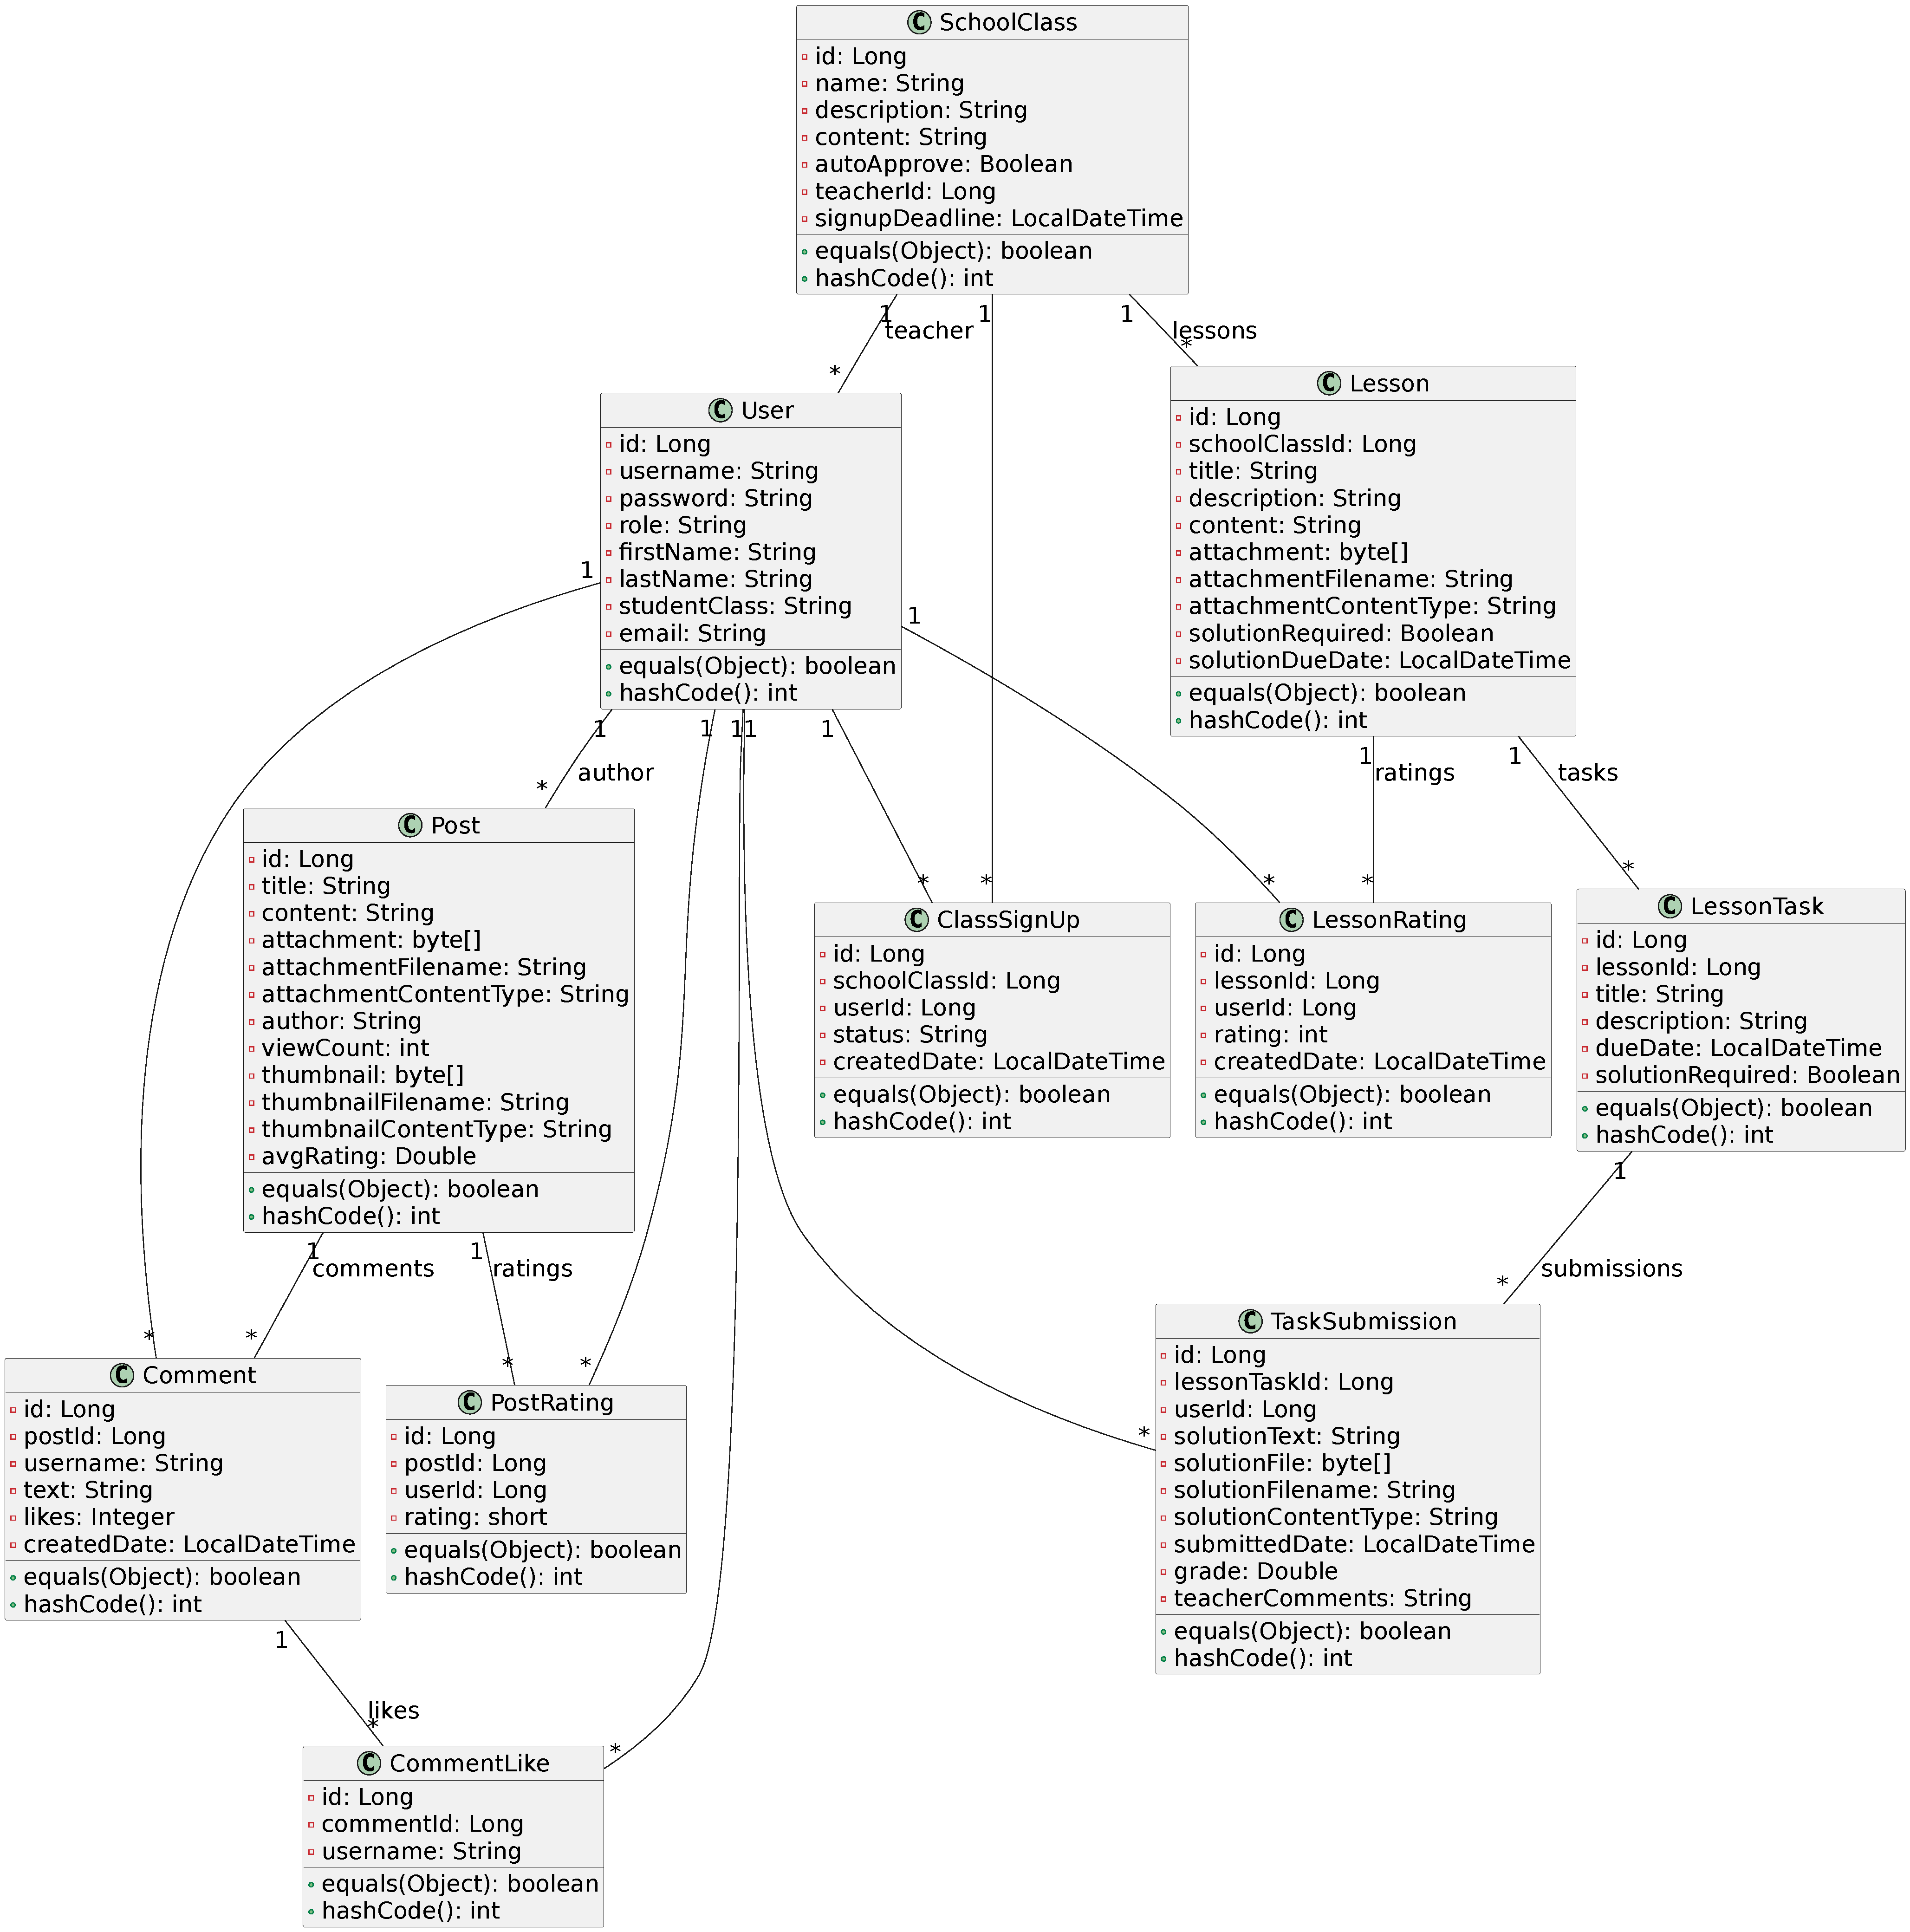
\includegraphics[width=\linewidth]{Dyplom-styl/svg-32.pdf} % Make sure this filename is correct and it's a PDF
    \caption{Diagram klas, Źródło: opracowanie własne}
    \label{fig:system_klas_zadan}
\end{figure}
Diagram skupia się wyłącznie na klasach domenowych i ich zależnościach do tych klas należą User, SchoolClass, Lesson, LessonTask, TaskSubmission, Post, Comment, PostRating, CommentLike, ClassSignUp, LessonRating. Na diagramie można zauważyć że użytkownik zapisuje się do klasy przez ClassSignup, lekcja agreguje zadania, a oceny i polubienia są encjami asocjacyjnymi. Przyjęto, że tylko nauczyciel i admin tworzą lekcje, zadania, dodają Posty i oceniają rozwiązania wysłane przez użytkowników, zaś użytkownicy mogą składać rozwiązania wystawiać oceny lekcją i postom i dodają komentarze, co wprost wynika z kierunku asocjacji i ról widocznych na diagramie
\begin{figure}[H]
  \centering
  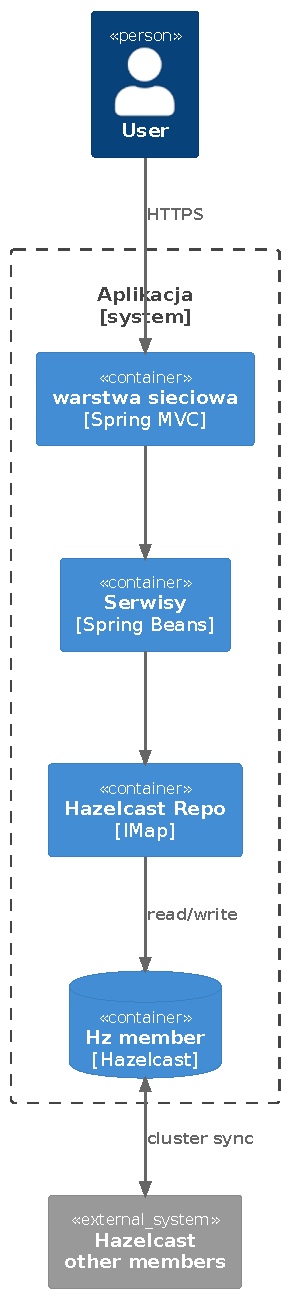
\includegraphics[
        width=\linewidth,
        height=0.8\textheight,   % nie przekrocz 80 % wysokości strony
        keepaspectratio          % zachowaj proporcje
  ]{Dyplom-styl/sv-10.pdf}
  \caption{Diagram komponentów Źródło: opracowanie własne}
  \label{fig:system_klas_zadan}
\end{figure}
diagram pokazuje przepływ: Klient->Web->Serwis->Repo->Hazelcast<->Klaster, użytkownik komunikuje się z systemem przez protokół HTTPS. Warstwe sieciową aplikacji tworzą kontrolery, wykonywana jest tam również walidacja żądań. serwisy tworzą logike domenową, hazelcast repo tworzy warstwe dostępu do danych. Operacje czytania i zapisywania są wykonywane na węźle klastra Hazelcast działającym w aplikacji, natomiast Hazelcast other members pozostałe węzły klastra. Dane są synchronizowane w klastrze.
\begin{figure}[H]
  \centering
  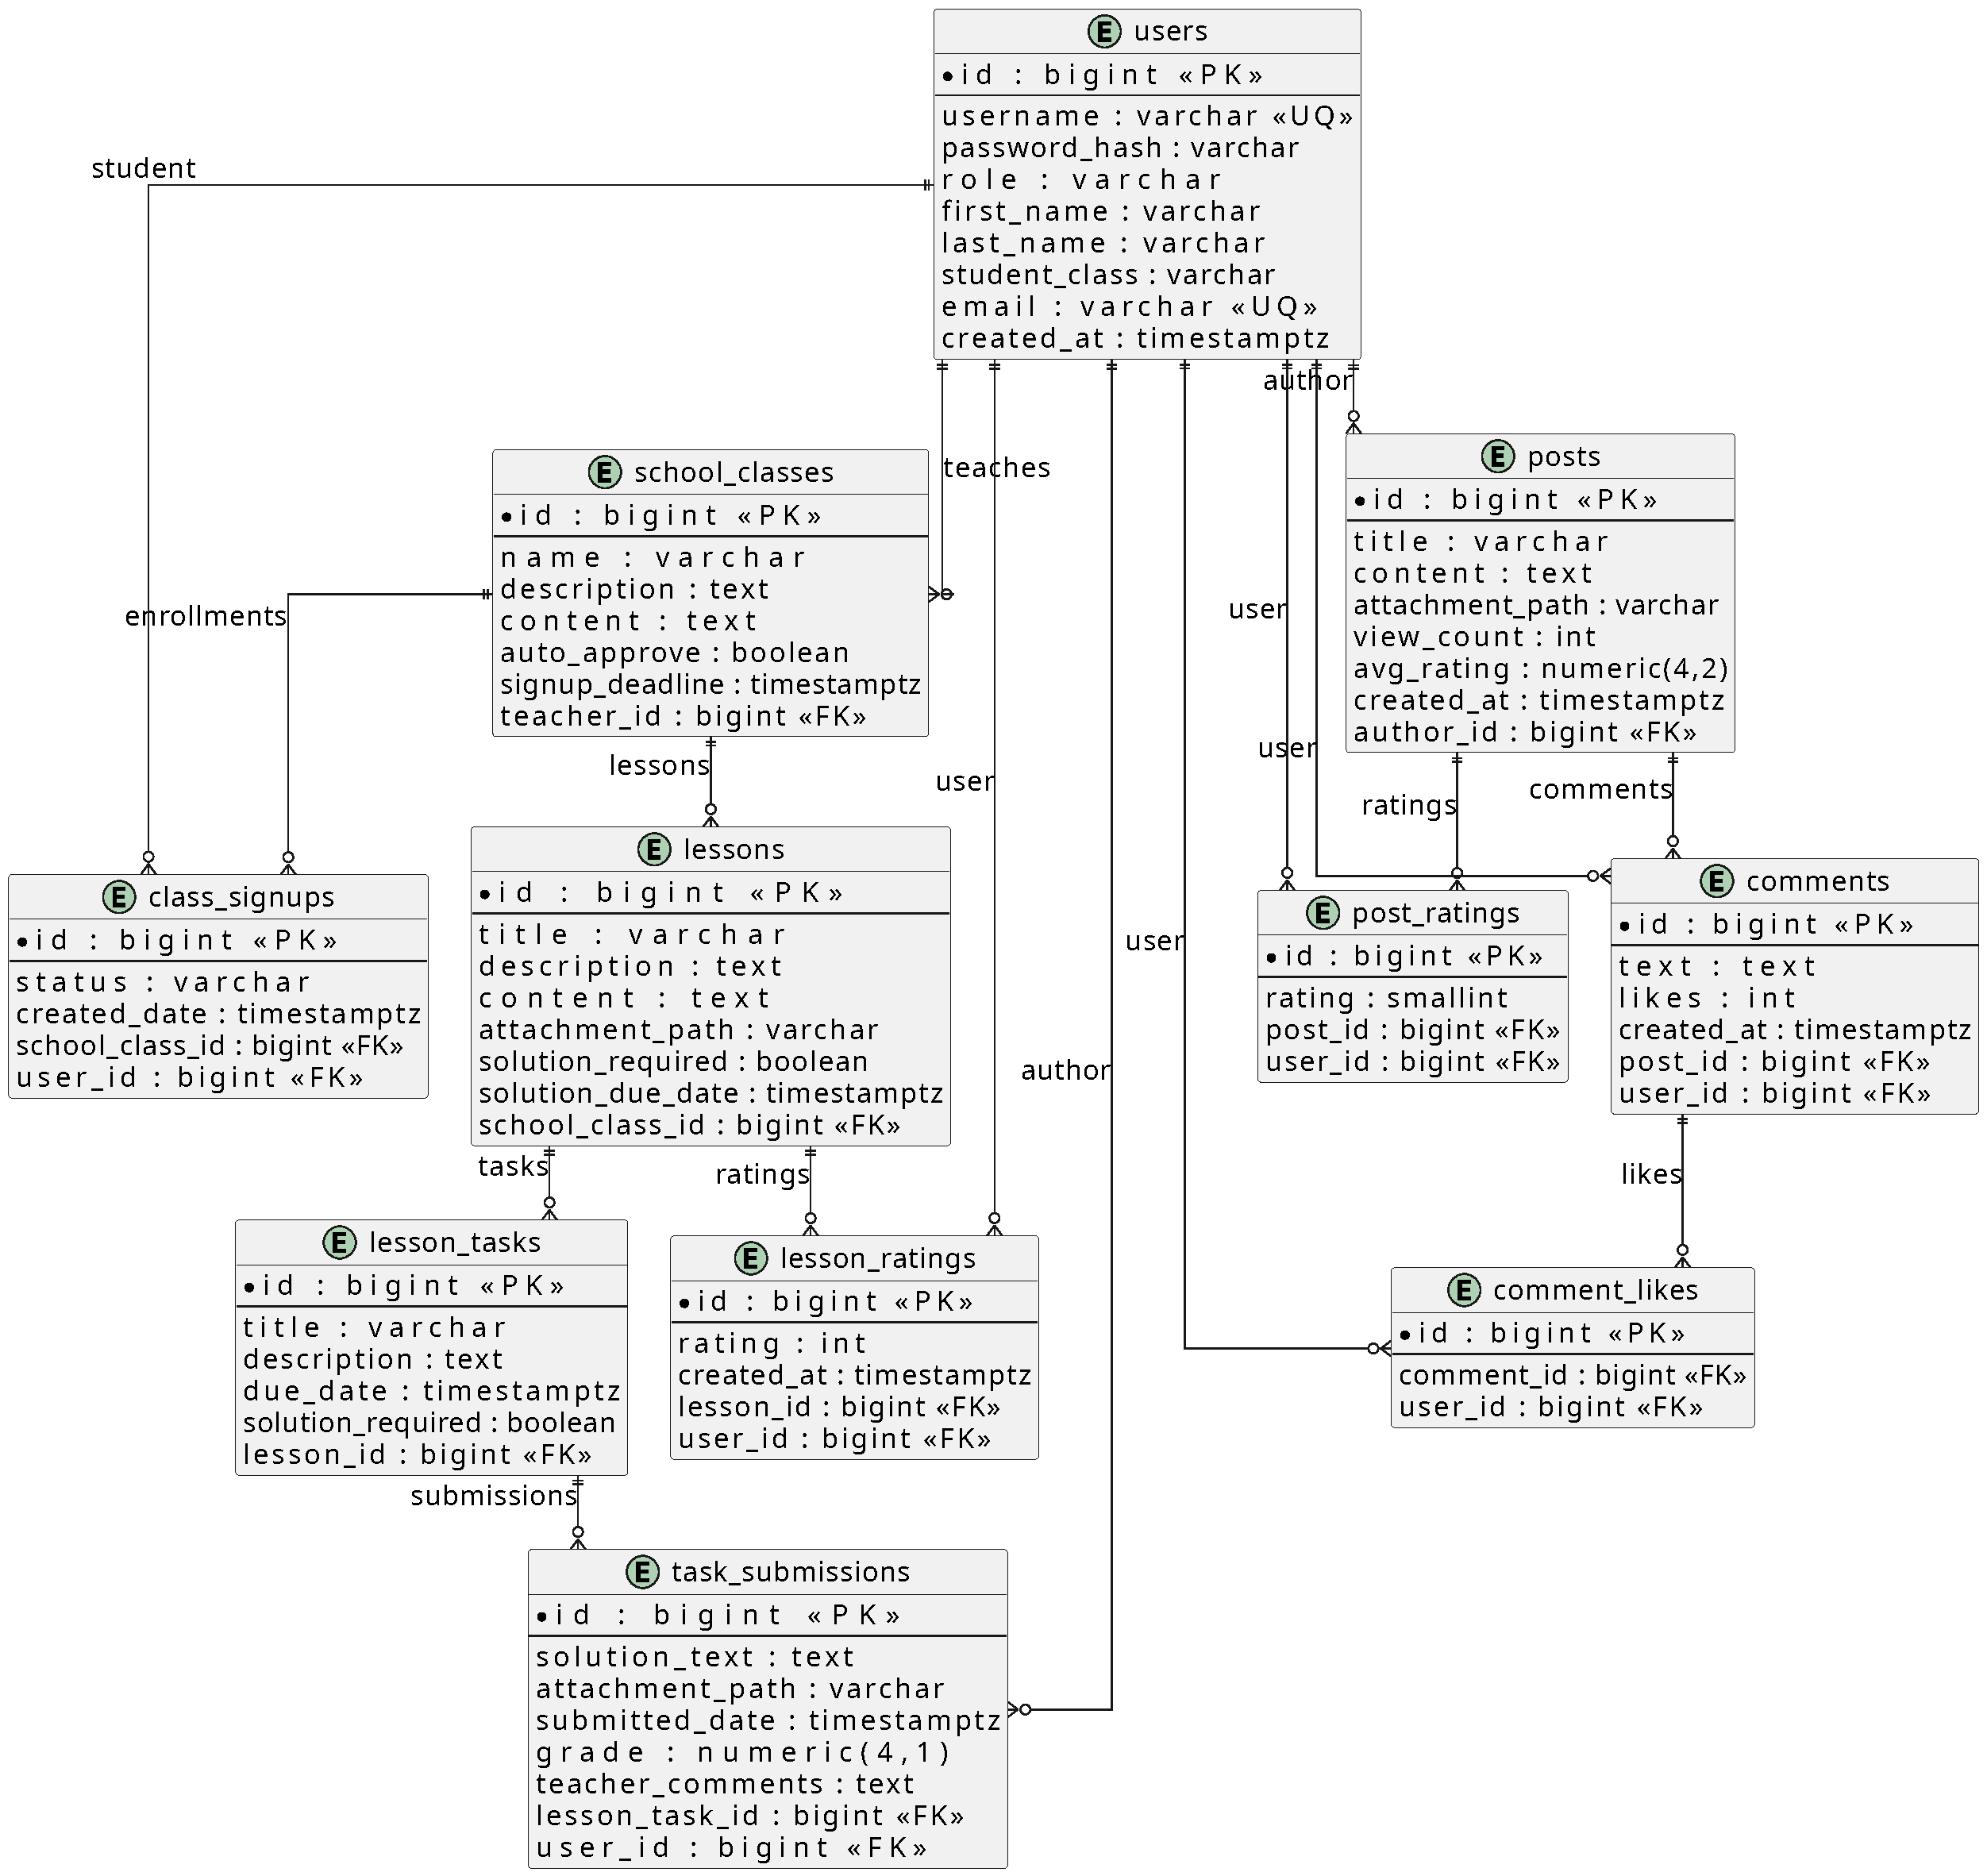
\includegraphics[
        width=\linewidth,
        height=0.8\textheight,   % nie przekrocz 80 % wysokości strony
        keepaspectratio          % zachowaj proporcje
  ]{Dyplom-styl/erd-22.pdf}
  \caption{Diagram ERD Źródło: opracowanie własne}
  \label{fig:system_klas_zadan}
\end{figure}
Diagram pokazuje powiązania pomiędzy tabelami w bazie danych, \begin{itemize}
    \item \texttt{users}: użytkownicy, unikalne pola to \texttt{username} i \texttt{email} zawiera również pola przechowujące imie nazwisko role i hasło.
    \item \texttt{school\_classes}: klasy, z kluczem obcym \texttt{teacher\_id}, który odnosi się do tabeli \texttt{users}.
    \item \texttt{class\_signups}: zapisy do klas, zawiera dwa klucze obce: \texttt{user\_id} oraz \texttt{school\_class\_id}, a także pola statusu i daty.
    \item \texttt{lessons}: lekcja, zawiera \texttt{school\_class\_id}, \texttt{user\_id}, treść, załącznik, termin oddania oraz informację, czy jest dodane zadanie do lekcji.
    \item \texttt{lesson\_tasks}: zadanie przypisane do lekcji (\texttt{lesson\_id}), z terminem i informacją o tym, czy jest wymagane.
    \item \texttt{task\_submissions}: rozwiązania przesłane przez użytkowników (\texttt{lesson\_task\_id}, \texttt{user\_id}), opcjonalny plik bądź tekst, data wysłania, ocena oraz komentarz nauczyciela.
    \item \texttt{lesson\_rating}: oceny lekcji, zawiera dwa klucze obce: \texttt{lesson\_id} i \texttt{user\_id}, oraz pole rating czyli ocenę lekcji.
    \item \texttt{posts}: posty zawierają: autora, treść, ścieżkę załącznika, liczbę wyświetleń oraz średnią ocenę z ocen wystawionych przez użytkowników.
    \item \texttt{comments}: komentarze do postów, z treścią i liczbą polubień.
    \item \texttt{post\_ratings}: oceny postów, z kluczami obcymi \texttt{post\_id} i \texttt{user\_id}, oraz polem rating.
    \item \texttt{comment\_likes}: polubienia komentarzy, zawiera, klucz obcy commentId oraz username.
\end{itemize}
\begin{figure}[H]
  \centering
  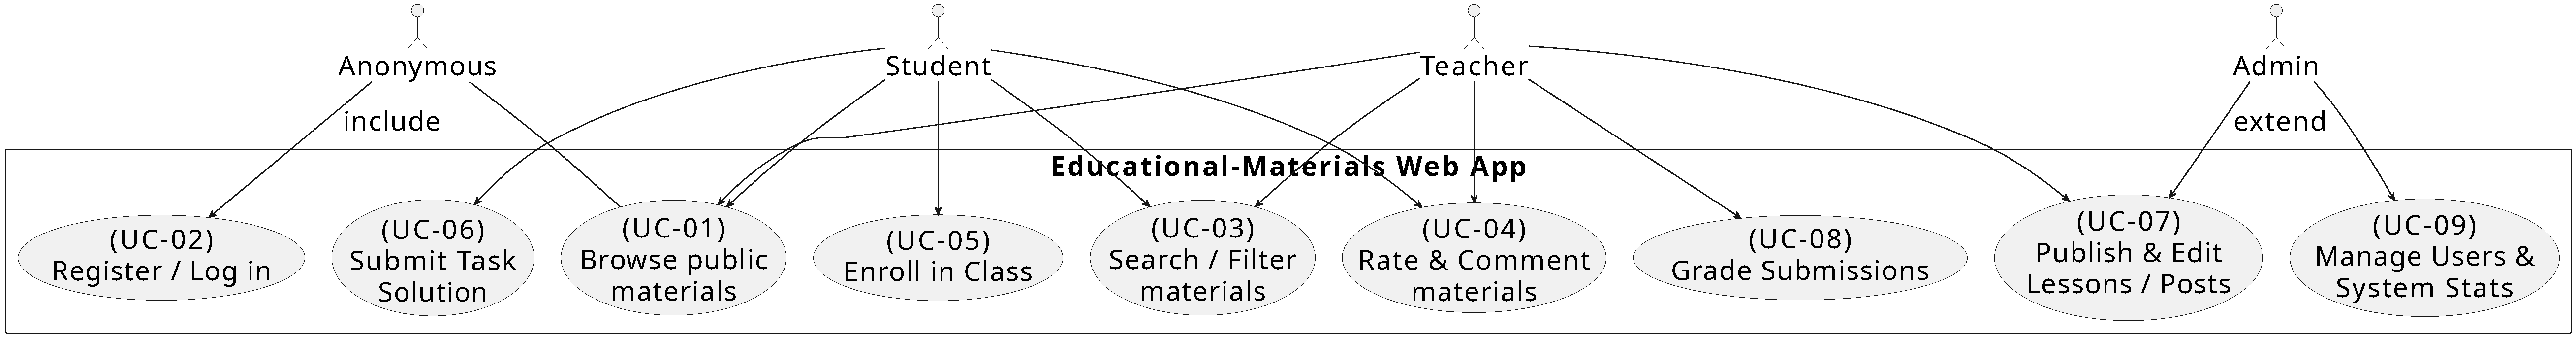
\includegraphics[
        width=\linewidth,
        height=0.8\textheight,   % nie przekrocz 80 % wysokości strony
        keepaspectratio          % zachowaj proporcje
  ]{Dyplom-styl/useCase-1-35.pdf}
  \caption{Diagram przypadków użycia -  ogólny zakres funkcjonalności platformy  Źródło: opracowanie własne}
  \label{fig:system_klas_zadan}
\end{figure}
Powyższy diagram przedstawia ogólny zakres funkcjonalności platformy materiałów edukacyjnych, ukazując kluczowe interakcje różnych użytkowników z systemem. Anonimowi użytkownicy mogą przeglądać publiczne materiały oraz rejestrować się i logować do systemu. Zarejestrowani studenci, oprócz przeglądania, mogą wyszukiwać i filtrować materiały, oceniać je i komentować, zapisywać się do klas oraz przesyłać rozwiązania zadań. Nauczyciele mają możliwość przeglądania i wyszukiwania materiałów, ich oceniania i komentowania, a także publikowania i edytowania własnych lekcji i postów oraz oceniania przesłanych zadań. Administratorzy odpowiadają za zarządzanie użytkownikami i statystykami systemowymi, a także mogą rozszerzać swoje działania o publikowanie i edytowanie materiałów.
\begin{figure}[H]
  \centering
  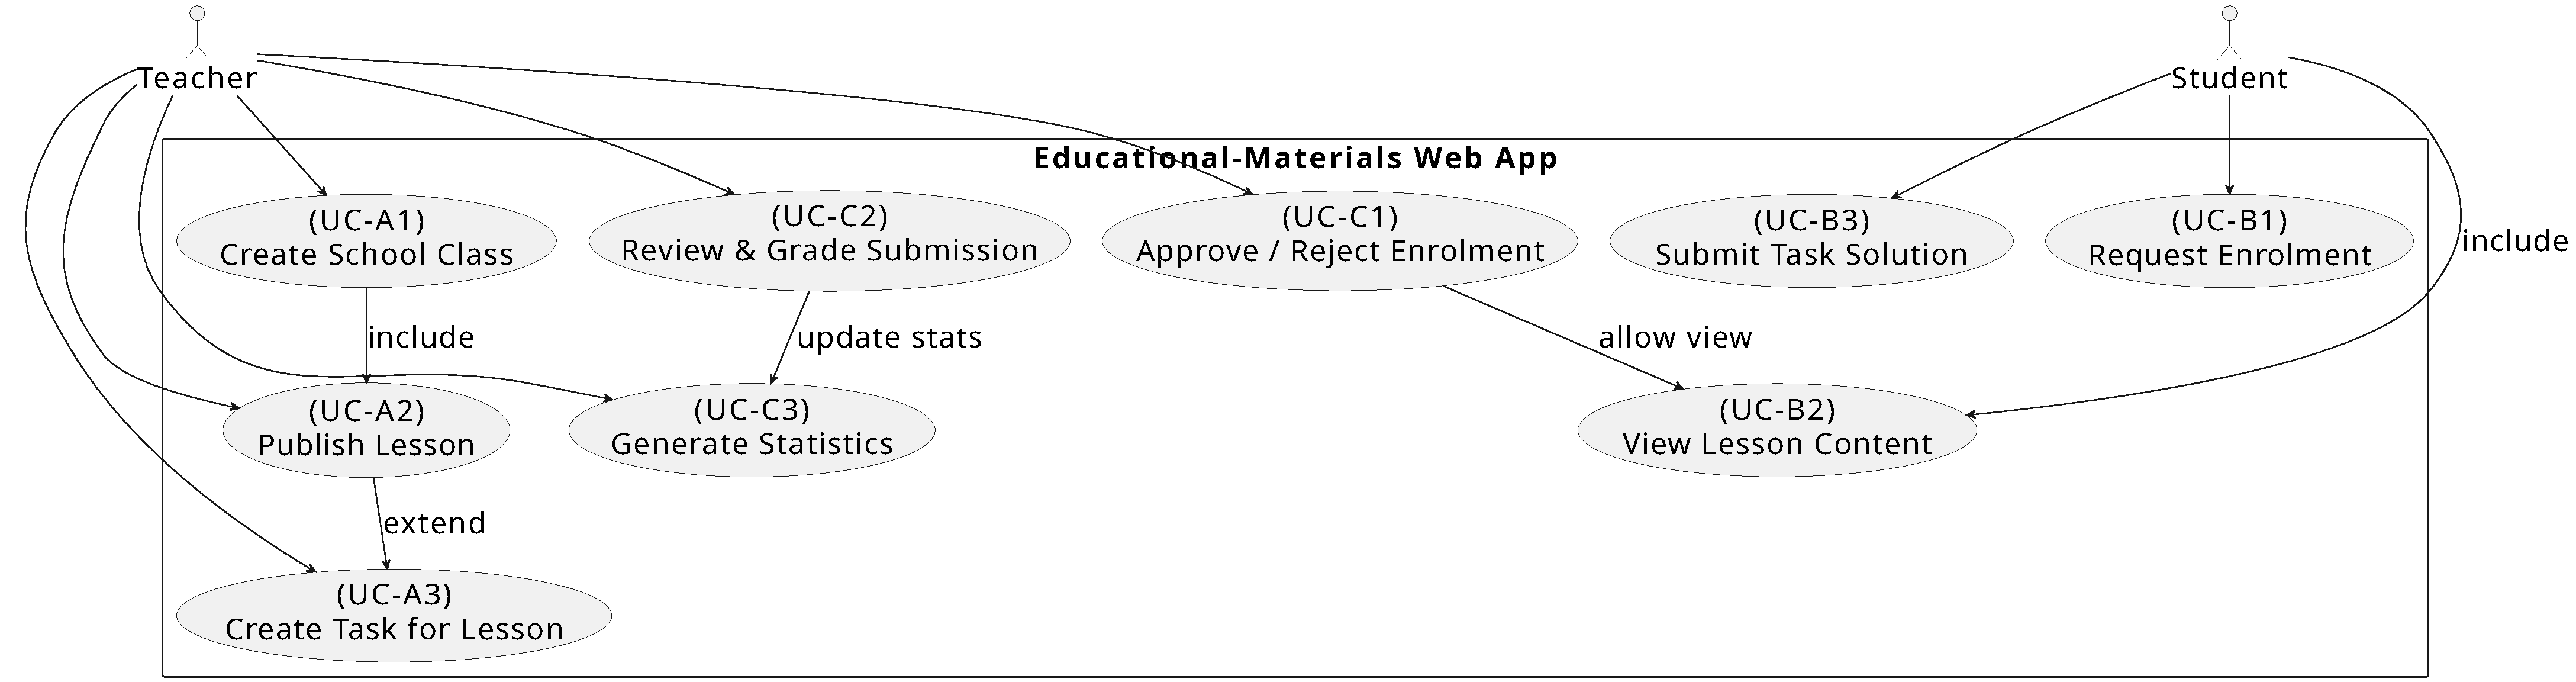
\includegraphics[
        width=\linewidth,
        height=0.8\textheight,   % nie przekrocz 80 % wysokości strony
        keepaspectratio          % zachowaj proporcje
  ]{Dyplom-styl/useCase-2-32.pdf}
  \caption{Diagram przypadków użycia - zarządzanie lekcjami i kursami Źródło: opracowanie własne}
  \label{fig:system_klas_zadan}
\end{figure}
Powyższy diagram koncentruje się na szczegółowym przebiegu interakcji między Nauczycielem a Studentem w kontekście zarządzania klasami, lekcjami i zadaniami. Nauczyciel może tworzyć nowe klasy, publikować lekcje, a następnie tworzyć zadania dla tych lekcji. Ma także uprawnienia do zatwierdzania lub odrzucania próśb o zapisanie się do klasy, przeglądania i oceniania przesłanych rozwiązań zadań, a także generowania statystyk. Student natomiast może prosić o zapisanie się do klasy, przeglądać zawartość lekcji oraz przesyłać rozwiązania zadań. Diagram ilustruje również, jak tworzenie klasy obejmuje publikację lekcji, publikacja lekcji. Zapisanie do klasy pozwala studentowi na przeglądanie zawartości lekcji, ocena zadań aktualizuje statystyki.

\begin{figure}[H]
  \centering
  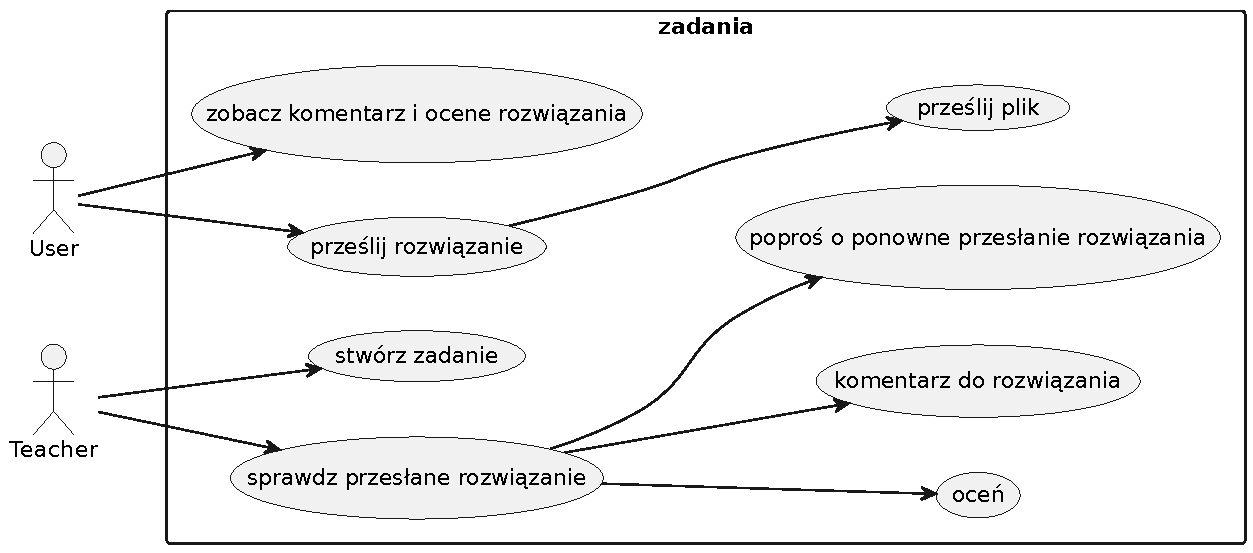
\includegraphics[
        width=\linewidth,
        height=0.8\textheight,   % nie przekrocz 80 % wysokości strony
        keepaspectratio          % zachowaj proporcje
  ]{Dyplom-styl/useCAse33.pdf}
  \caption{Diagram przypadków użycia -  przesyłanie i ocenianie rozwiązań do zadań  Źródło: opracowanie własne}
  \label{fig:system_klas_zadan}
\end{figure}
Powyższy diagram przedstawia przepływ akcji związanych z zadaniami. Nauczyciel tworzy zadanie do lekcji bedącej częścią klasy(przedmiotu) do którego uczeń(user) należy następnie uczeń przesyła rozwiązanie, nauczyciel wystawia ocene ewentualnie dodaje komentarz i na końcu użytkownik może sprawdzić ocene oraz komentarz dodany przez nauczyciela. % chapter3.tex zawiera treść rozdziału 3

%----------------------------------------------------------------------------------------
%	ROZDZIAŁ 4
%----------------------------------------------------------------------------------------
\chapter{Testowanie i ocena aplikacji}

W niniejszym rozdziale przedstawiono proces testowania aplikacji oraz ocenę poprawności jej działania. Omówione zostały podejścia wykorzystane w testach jednostkowych oraz integracyjnych, a także ocena wydajności aplikacji.

\section{Wprowadzenie do testowania aplikacji}

Testowanie stanowi kluczowy element procesu tworzenia oprogramowania, umożliwiający wykrycie błędów oraz weryfikację poprawności działania zaimplementowanych funkcjonalności. W ramach tej aplikacji wykorzystano dwa główne rodzaje testów:

\begin{itemize}
    \item Testy jednostkowe – testujące pojedyncze klasy oraz metody.
    \item Testy integracyjne – sprawdzające poprawność współdziałania wielu komponentów systemu.
\end{itemize}

\section{Testy jednostkowe}

Testy jednostkowe zostały napisane z użyciem frameworka JUnit 5, który jest szeroko stosowany w aplikacjach Java ze względu na łatwość integracji ze środowiskiem Spring Boot. 

Przykładowe testy jednostkowe objęły klasy:

\begin{itemize}
    \item Serwisy (np. \texttt{StatsService}), które weryfikują poprawność operacji na danych.
    \item Klasy DAO (np. \texttt{StatsDaoImpl}), które sprawdzają prawidłowe wykonanie zapytań SQL do bazy danych H2.
    \item Kontrolery, gdzie przy pomocy MockMVC testowano poprawność zwracanych widoków oraz danych.
\end{itemize}

\subsection{Przykład testu jednostkowego}

Poniżej przedstawiono przykład testu jednostkowego dla klasy \texttt{StatsService}:

\begin{lstlisting}[language=Java]
@Test
void shouldUpdateStatisticsCorrectly() {
    when(postRepository.count()).thenReturn(10L);
    when(userRepository.countByRole("TEACHER")).thenReturn(2L);

    statsService.updateStatistics();

    verify(statsDao, times(1)).saveStat(any(AppStatistic.class));
}
\end{lstlisting}

Wykorzystanie mechanizmów \texttt{Mockito} pozwoliło na izolację testowanych metod od zewnętrznych zależności.

\section{Testy integracyjne}

Testy integracyjne przeprowadzono z wykorzystaniem frameworka Spring Boot oraz wbudowanej bazy danych H2. Głównym celem było sprawdzenie poprawności współpracy różnych warstw aplikacji.

Do realizacji tych testów wykorzystano:

\begin{itemize}
    \item \texttt{TestRestTemplate} – do symulacji pełnych zapytań HTTP i sprawdzania zwracanych odpowiedzi.
    \item Spring Test – zapewniający kompleksową konfigurację środowiska testowego.
\end{itemize}

\subsection{Przykład testu integracyjnego}

Poniżej przedstawiono przykład testu integracyjnego sprawdzającego poprawność działania strony głównej aplikacji:

\begin{lstlisting}[language=Java]
@SpringBootTest(webEnvironment = SpringBootTest.WebEnvironment.RANDOM_PORT)
class ApplicationIntegrationTests {

    @Autowired
    private TestRestTemplate restTemplate;

    @Test
    void shouldLoadHomePageSuccessfully() {
        ResponseEntity<String> response = restTemplate.getForEntity("/", String.class);

        assertEquals(HttpStatus.OK, response.getStatusCode());
        assertTrue(response.getBody().contains("Educational Materials Sharing Platform"));
    }
}
\end{lstlisting}

Testy integracyjne potwierdziły poprawne współdziałanie komponentów aplikacji.

\section{Baza danych testowa (H2)}

W trakcie realizacji testów wykorzystano bazę danych H2 działającą w pamięci, która umożliwiła szybkie i bezpieczne wykonywanie operacji CRUD, bez ingerencji w dane produkcyjne. Baza ta została również użyta do przechowywania sesji użytkowników oraz tymczasowych statystyk aplikacji. 

Przykładowa konfiguracja użytej bazy danych:

\begin{lstlisting}[language=properties]
spring.datasource.url=jdbc:h2:mem:testdb
spring.datasource.driverClassName=org.h2.Driver
spring.datasource.username=sa
spring.datasource.password=
spring.jpa.database-platform=org.hibernate.dialect.H2Dialect
\end{lstlisting}

\section{Testy wydajnościowe}

Do oceny wydajności aplikacji przeprowadzono podstawowe testy wydajnościowe, które polegały na symulacji dużego obciążenia generowanego przez jednoczesne zapytania użytkowników. Wyniki wykazały stabilność aplikacji pod obciążeniem oraz akceptowalne czasy odpowiedzi.

Testy przeprowadzono przy użyciu narzędzi takich jak Apache JMeter. Przykładowe parametry testu:

\begin{itemize}
    \item Liczba jednoczesnych użytkowników: 100.
    \item Czas trwania testu: 10 minut.
    \item Średni czas odpowiedzi aplikacji: poniżej 300ms.
\end{itemize}

Wnioski z testów pokazały, że aplikacja działa wydajnie i jest zdolna obsłużyć przewidywaną liczbę użytkowników.

\section{Podsumowanie wyników testów}

Przeprowadzone testy jednostkowe i integracyjne potwierdziły poprawność działania aplikacji oraz jej zgodność z założonymi wymaganiami funkcjonalnymi. Testy wydajnościowe dodatkowo potwierdziły stabilność aplikacji przy dużym obciążeniu, co umożliwia jej efektywne wdrożenie w środowisku edukacyjnym.
 % chapter4.tex zawiera treść rozdziału 4

%----------------------------------------------------------------------------------------
%	ROZDZIAŁ 5
%----------------------------------------------------------------------------------------
\chapter{Implementacja}

Ten rozdział omawia szczegółowe aspekty implementacji platformy do udostępniania materiałów edukacyjnych, obejmujące konfigurację środowiska, logikę backendu, integrację frontendową oraz mechanizmy przechowywania danych użyte w projekcie.

\section{Konfiguracja środowiska}

Środowisko deweloperskie zostało przygotowane przez dobór odpowiednich narzędzi, frameworków oraz technologii, które umożliwiają szybkie tworzenie aplikacji, wysoką produktywność oraz solidną architekturę systemu. W projekcie wykorzystano następujące narzędzia i technologie:

\begin{itemize}
\item \textbf{Język programowania}: Java 21
\item \textbf{Framework}: Spring Boot 3.x
\item \textbf{Narzędzie do budowania aplikacji}: Apache Maven
\item \textbf{IDE}: IntelliJ IDEA
\item \textbf{Systemy bazodanowe}: PostgreSQL (dane trwałe) oraz H2 Database (w pamięci, używana do statystyk, testowania i zarządzania sesjami)
\item \textbf{Technologie webowe}: Thymeleaf, Bootstrap 5.2, JavaScript
\item \textbf{System kontroli wersji}: Git
\end{itemize}

Zależności zarządzane były za pomocą pliku \texttt{pom.xml} Maven, zapewniając prostą integrację bibliotek zewnętrznych, takich jak Spring Web, Spring Security, JDBC, Thymeleaf oraz frameworków testowych (JUnit, Mockito).

\section{Rozwój backendu}

Backend aplikacji opiera się na architekturze warstwowej, obejmującej kontrolery, serwisy, obiekty dostępu do danych (DAO) oraz repozytoria. Podejście to zapewnia wyraźny podział odpowiedzialności, łatwiejsze utrzymanie oraz testowalność.

\subsection{Uwierzytelnianie i autoryzacja użytkowników}

Uwierzytelnianie użytkowników oraz autoryzacja oparta na rolach zostały zrealizowane za pomocą Spring Security. Hasła są szyfrowane z wykorzystaniem algorytmu haszującego BCrypt, zwiększając bezpieczeństwo.

Zaimplementowane role:

\begin{itemize}
\item \textbf{Student} – może przeglądać materiały oraz przesyłać rozwiązania.
\item \textbf{Nauczyciel} – może dodawać materiały oraz oceniać przesłane rozwiązania.
\item \textbf{Administrator} – zarządza użytkownikami oraz statystykami systemu.
\end{itemize}

Spring Security został skonfigurowany do zabezpieczenia URL na podstawie ról użytkowników, dostarcza również funkcjonalności logowania, wylogowania oraz zarządzania sesjami.

\subsection{Kontrolery MVC i serwisy}

Kontrolery zarządzają żądaniami oraz odpowiedziami HTTP według wzorca Spring MVC. Kontrolery delegują logikę biznesową do warstw serwisowych, co utrzymuje klarowny podział między obsługą żądań a operacjami biznesowymi.

Przykład implementacji (fragment kontrolera):

\begin{lstlisting}[language=Java]
@GetMapping("/classes/{classId}/lessons")
public String viewLessons(@PathVariable Long classId, Model model) {
List lessons = lessonService.getLessonsForClass(classId);
model.addAttribute("lessons", lessons);
return "lessons";
}
\end{lstlisting}

Serwisy realizują logikę transakcyjną oraz współpracują z repozytoriami i DAO, aby pobierać i manipulować danymi.

\subsection{Repozytoria i DAO}

Trwałe dane przechowywane są w bazie PostgreSQL, do której dostęp zapewniają repozytoria Spring Data JDBC. Dane tymczasowe, takie jak statystyki aplikacji oraz sesje użytkowników, obsługiwane są przez bazę H2 w pamięci, za pośrednictwem własnych implementacji DAO.

Przykład implementacji DAO:

\begin{lstlisting}[language=Java]
@Repository
public class StatsDaoImpl implements StatsDaoImplRepository {

private final NamedParameterJdbcOperations jdbcOperations;

@Autowired
public StatsDaoImpl(@Qualifier("tempJdbcTemplate") NamedParameterJdbcOperations jdbcOperations) {
    this.jdbcOperations = jdbcOperations;
}

public List<AppStatistic> findAllStats() {
    String sql = "SELECT id, stat_name, stat_value, timestamp FROM app_statistics";
    return jdbcOperations.query(sql, new BeanPropertyRowMapper<>(AppStatistic.class));
}

}
\end{lstlisting}

\subsection{Zadania cykliczne}

Aplikacja wykorzystuje zadania cykliczne (za pomocą Spring Scheduler) do regularnego aktualizowania statystyk aplikacji, takich jak liczba postów, zarejestrowanych użytkowników oraz aktywność użytkowników. Statystyki te przechowywane są w bazie H2 i używane są do analiz administracyjnych.

\begin{lstlisting}[language=Java]
@Component
public class StatisticsUpdater {

@Autowired
private StatsService statsService;

@Scheduled(cron = "*/30 * * * * *")
public void updateStats() {
    statsService.updateStatistics();
}

}
\end{lstlisting}

\section{Rozwój frontendu}

Frontend został zbudowany z użyciem szablonów Thymeleaf, umożliwiających dynamiczne renderowanie treści bezpośrednio z kontrolerów Spring MVC. Framework Bootstrap zapewnia responsywny oraz estetyczny interfejs użytkownika.

\subsection{Integracja z Thymeleaf}

Thymeleaf oferuje przejrzystą integrację ze Spring Boot, umożliwiając łatwe wiązanie danych i renderowanie danych po stronie serwera:

Przykładowy fragment Thymeleaf:

\begin{lstlisting}[language=HTML]

\subsection{Wykorzystanie komponentów Bootstrap}

Do stylowania wykorzystano Bootstrap 5, upraszczając obsługę CSS oraz zapewniając spójny design na różnych urządzeniach.

\section{Zarządzanie przechowywaniem danych}

W projekcie użyto dwóch baz danych:

\begin{itemize}
\item \textbf{PostgreSQL} – przechowuje dane trwałe, takie jak użytkownicy, posty, komentarze, lekcje oraz zadania.
\item \textbf{H2 Database} – do przechowywania danych tymczasowych, danych sesji, statystyk aplikacji oraz celów testowych.
\end{itemize}

Baza H2 jest inicjalizowana podczas startu aplikacji za pomocą skryptów schematu oraz danych, co pozwala na szybkie testowanie bez wpływu na dane produkcyjne.

Przykładowa konfiguracja bazy H2 w pliku \texttt{application.properties}:

\begin{lstlisting}[language=properties]
spring.datasource.temp.url=jdbc:h2:mem:tempdb;DB_CLOSE_DELAY=-1
spring.datasource.temp.username=sa
spring.datasource.temp.password=
spring.datasource.temp.driver-class-name=org.h2.Driver
\end{lstlisting}

\section{Wyzwania implementacyjne i ich rozwiązania}

Podczas implementacji pojawiło się kilka wyzwań, które rozwiązano następująco:

\begin{itemize}
\item \textbf{Spójność danych pomiędzy bazami PostgreSQL i H2} – rozwiązana przez jasne określenie odpowiedzialności każdej bazy.
\item \textbf{Synchronizacja zadań cyklicznych} – rozwiązana poprzez właściwą konfigurację wyrażeń cron i izolację zadań.
\item \textbf{Integracja backendu z frontendem} – rozwiązana przez dokładne wykorzystanie możliwości renderowania po stronie serwera Thymeleaf.
\end{itemize}

\section{Podsumowanie}

Implementacja platformy do udostępniania materiałów edukacyjnych wykazała efektywne wykorzystanie nowoczesnych technologii oraz frameworków takich jak Spring Boot, PostgreSQL oraz baza danych H2. Ukazała również skuteczne rozwiązania dla typowych wyzwań programistycznych, zapewniając stabilność, bezpieczeństwo oraz przyjazność użytkownikowi stworzonej aplikacji.

 % chapter5.tex zawiera treść rozdziału 5

%----------------------------------------------------------------------------------------
%	ROZDZIAŁ 6
%----------------------------------------------------------------------------------------
\chapter{Testowanie i ocena aplikacji} W niniejszym rozdziale przedstawiono proces testowania aplikacji oraz ocenę poprawności jej działania pod względem funkcjonalnym i niefunkcjonalnym. Omówione zostały podejścia wykorzystane w testach jednostkowych, integracyjnych, testy wydajnościowe oraz testy end-to-end. Celem testowania było upewnienie się, że wszystkie warstwy systemu współpracują prawidłowo, a aplikacja spełnia postawione wymagania w warunkach zbliżonych do rzeczywistych obciążeń. \section{Wprowadzenie do testowania aplikacji} Testowanie stanowi kluczowy element procesu tworzenia oprogramowania, umożliwiający wykrycie błędów oraz weryfikację poprawności zaimplementowanych funkcjonalności na wczesnym etapie. W ramach tego projektu zastosowano różne poziomy testów, aby uzyskać pewność co do jakości kodu: \begin{itemize}
\item \textbf{Testy jednostkowe} –Testy jednostkowe sprawdzają pojedyncze jednostki kodu. Pozwalają sprawdzić logikę wybranego fragmentu kodu w oderwaniu od kontekstu aplikacji (np. metodę serwisu aktualizującą statystyki lub walidującą dane wejściowe) \cite{effective-unit-testing}.
\item \textbf{Testy integracyjne} – sprawdzają, czy współpraca wielu komponentów (warstwa web, logika, dostęp do danych, mechanizmy bezpieczeństwa) przebiega poprawnie w uruchomionym kontekście aplikacji. \cite{spring-docs}
\item \textbf{Testy wydajnościowe} – oceniają zachowanie aplikacji przy wzrastającym obciążeniu i równoległych użytkownikach, aby upewnić się, że czasy odpowiedzi mieszczą się w akceptowalnych granicach \cite{jmeter-docs}.
\end{itemize} Tak wielopoziomowe podejście do testowania umożliwia wykrycie różnych klas błędów od drobnych pomyłek w logice pojedynczej metody, przez problemy z konfiguracją kontekstu Spring, aż po ewentualne wąskie gardła w wydajności. \section{Testy jednostkowe} Testy jednostkowe zostały napisane z użyciem frameworka JUnit 5, który jest obecnie standardem w ekosystemie Java. Do izolowania zależności wykorzystano bibliotekę Mockito, pozwalającą na tworzenie próbnych obiektów (moków) zastępujących np. warstwę repozytorium podczas testowania serwisu, lub warstwę serwisu podczas testowania kontrolera \cite{mockito-docs}. Dzięki temu można skupić się na logice danej jednostki kodu, nie przejmując się działaniem pozostałych komponentów (które są zasymulowane). Przykładowo, testy jednostkowe objęły klasy:
\begin{itemize}
\item \textbf{Serwisy} – np. \texttt{StatsService}, gdzie sprawdzono czy metoda aktualizująca statystyki poprawnie odczytuje dane z repozytoriów i zapisuje zaktualizowane statystyki. Zastosowano tutaj \textit{stub} na metodach repozytoriów \cite{mockito-docs, junit-docs}(\texttt{postRepository}, \texttt{userRepository}, itp.) zwracające z góry ustalone wartości, by zasymulować określony stan systemu, a następnie weryfikowano, czy serwis wywołuje metodę zapisu statystyk dokładnie raz z poprawnymi parametrami.
\item \textbf{Kontrolery} – testowane zarówno metodami bezpośredniego wywołania, jak i z użyciem Spring MockMVC. W pierwszym podejściu tworzono instancję kontrolera i za pomocą moków podstawiano zależności (np. \texttt{UserRepository}, \texttt{PasswordEncoder}), a następnie wywoływano metodę kontrolera tak, jakby obsługiwała żądanie. Sprawdzano zwracany widok oraz efekty uboczne (np. czy nowy użytkownik został zapisany w repozytorium po rejestracji). W drugim podejściu (MockMVC) uruchamiano wbudowany serwer Tomcat w trybie testowym i wykonywano sztuczne zapytania HTTP do endpointów, sprawdzając kod odpowiedzi i fragmenty wygenerowanej strony. \cite{spring-docs}
\item \textbf{Repozytoria} – ponieważ repozytoria Hazelcast nie korzystają z klasycznego mechanizmu ORM ani bazy SQL, testy jednostkowe repozytoriów polegały głównie na sprawdzeniu logiki metod filtrujących. Np. \texttt{ClassSignUpRepository.findBySchoolClassIdAndUserId} filtruje kolekcję zapisów, więc utworzono kilka obiektów \texttt{ClassSignUp} w kontrolowanej mapie i upewniono się, że metoda znajduje właściwy obiekt lub zwraca \texttt{Optional.empty()} gdy brak dopasowania \cite{hazelcast-docs}.
\end{itemize}
Poniżej przedstawiono fragment przykładowego testu jednostkowego dla serwisu statystyk \texttt{StatsService}, demonstrującego użycie Mockito do symulacji repozytoriów i weryfikacji zachowania:
\begin{lstlisting}[language=Java,
  caption={test kodu aktualizowania statystyk. Źródło: opracowanie własne},
  label={lst:testStatisticUpdater},
  captionpos=b]
@Test
void shouldUpdateStatisticsCorrectly() {
// Symulacja wartości zwracanych przez repozytoria:
when(postRepository.count()).thenReturn(10L);
when(userRepository.countByRole("TEACHER")).thenReturn(2L);
when(userRepository.countByRole("USER")).thenReturn(5L);
when(commentRepository.count()).thenReturn(20L);
// Wywołanie testowanej metody:
statsService.updateStatistics();
// Weryfikacja, że statystyki zostały zapisane (4 statystyki do zapisania):
verify(statsRepository, times(4)).save(any(AppStatistic.class));
}
\end{lstlisting} W powyższym teście założono, że w systemie jest 10 postów, 2 nauczycieli, 5 zwykłych użytkowników i 20 komentarzy. Po wywołaniu \texttt{updateStatistics()} oczekujemy, że serwis spróbuje zapisać każdą z czterech statystyk (postCount, teacherCount, userCount, commentCount) dokładnie raz – stąd \texttt{verify} z \texttt{times(4)} na \texttt{statsRepository.save(...)}. Wykorzystanie mechanizmów Mockito pozwoliło na izolację testowanej metody od faktycznej bazy danych i innych serwisów  test jest szybki i deterministyczny. \section{Testy integracyjne} Testy integracyjne przeprowadzono z wykorzystaniem wbudowanych możliwości Spring Boot Test. Uruchamiając kontekst całej aplikacji w trybie testowym, można symulować rzeczywiste scenariusze użytkownika, sprawdzając czy wszystkie warstwy (od kontrolera, przez serwisy, po repozytoria i magazyn danych) działają wspólnie poprawnie. W projekcie wykorzystano głównie podejście \textbf{end-to-end}, gdzie testy integracyjne zachowywały się jak klienci aplikacji korzystający z niej przez protokół HTTP. Do realizacji takich testów zastosowano:
\begin{itemize}
  \item \texttt{SpringBootTest} z \texttt{webEnvironment=RANDOM\_PORT} --
dzięki \texttt{RANDOM\_PORT} testy uruchamiają aplikację na wolnym porcie, co pozwala na rzeczywisty dostęp HTTP do endpointów.
  \item \texttt{TestRestTemplate} --  klient HTTP z pakietu Spring Boot Test, umożliwiający wykonywanie żądań HTTP do uruchomionej aplikacji.
  \item profil \texttt{test} -- w testach aktywowano profil testowy, który
    używa osobnej konfiguracji Hazelcast (mniejsza liczba danych
    inicjalnych, wyłączone zadania cykliczne poprzez
    \texttt{spring.task.scheduling.enabled=false}, aby testy były
    deterministyczne).
\end{itemize}
 Przykładem testu integracyjnego może być sprawdzenie działania strony głównej aplikacji: \begin{lstlisting}[language=Java,
  caption={integracyjny test. Źródło: opracowanie własne},
  label={lst:integrationTest},
  captionpos=b]
@SpringBootTest(webEnvironment = SpringBootTest.WebEnvironment.RANDOM_PORT)
@ActiveProfiles("test")
class ApplicationIntegrationTests {
@Autowired
private TestRestTemplate restTemplate;
@Test
void homePageShouldLoadSuccessfully() {
ResponseEntity<String> response = restTemplate.getForEntity("/", String.class);
assertEquals(HttpStatus.OK, response.getStatusCode());
assertTrue(response.getBody().contains("Welcome to MyEduShare"));
}
}
\end{lstlisting} 
W powyższym teście uruchamiamy aplikację, wykonujemy zapytanie GET na
\texttt{"/"} (strona główna) i sprawdzamy, czy odpowiedź ma kod 200OK oraz
czy zwrócona treść HTML zawiera oczekiwany fragment (np. tytuł lub
charakterystyczny tekst powitalny strony). Taki test potwierdza, że
podstawowa ścieżka (wejście na stronę główną) działa prawidłowo-- aplikacja
się uruchamia, kontroler główny zwraca widok, a mechanizmy szablonów
poprawnie generują stronę.

Bardziej złożone testy integracyjne zostały stworzone dla typowych
scenariuszy użycia, opisanych w poprzednim rozdziale. Na przykład
przygotowano test end-to-end symulujący cały przepływ:
\textit{nauczyciel tworzy nowy kurs i zadanie $\to$ student rejestruje się i
zapisuje na ten kurs $\to$ student przesyła rozwiązanie zadania $\to$
nauczyciel pobiera i ocenia rozwiązanie $\to$ sprawdzenie, że ocena jest
zapisana}. Tego typu test (zaimplementowany w klasie
\texttt{TeacherStudentFlowE2eTest}) wykorzystuje \texttt{TestRestTemplate}
do wykonywania kolejnych żądań POST/GET, naśladując akcje formularzy (np.
przesyłając dane rejestracji w żądaniu POST do
\texttt{/perform\_register}, logując różne konta poprzez
\texttt{TestRestTemplate} z odpowiednimi ciasteczkami sesyjnymi itp.) \cite{spring-docs}. Po
serii akcji test weryfikuje stan bazy-- np. sprawdza, czy w repozytorium
\texttt{TaskSubmissionRepository} pojawił się wpis z oceną nauczyciela. Takie
kompleksowe testy dają dużą pewność, że kluczowe funkcjonalności aplikacji
działają poprawnie w całym przekroju systemu.

W trakcie testów integracyjnych aplikacja korzystała z tej samej bazy
Hazelcast (tyle że w trybie „test”, z osobną konfiguracją) co w normalnym
działaniu. Oznacza to, że wszystkie
operacje na danych w testach były wykonywane również w pamięci (co
zapewniło szybkość testów i identyczne warunki działania jak w
środowisku produkcyjnym aplikacji). Podejście to upraszcza testy-- brak
translacji do innej technologii (SQL) oznacza, że testujemy dokładnie te
same ścieżki kodu co podczas realnego działania aplikacji \cite{hazelcast-docs}. Testy
integracyjne potwierdziły poprawne współdziałanie komponentów aplikacji:
wszystkie zaplanowane scenariusze (rejestracja, logowanie, dodawanie
postów, zapisy na kurs, przesyłanie zadań, oceny itp.) zakończyły się
wynikiem zgodnym z oczekiwaniami. Również obsługa błędnych ścieżek (np.
próba dostępu do zasobów bez autoryzacji, podwójna rejestracja z tym samym
e-mailem) została zweryfikowana-- aplikacja w takich przypadkach zwraca komunikaty lub kody błędów (kod 403) \cite{spring-docs}.

\section{Testy wydajnościowe}

Ostatnim etapem było zbadanie zachowania aplikacji pod obciążeniem. W tym celu przygotowano plan w Apache JMeter, który symuluje jednoczesne działania wielu użytkowników i pozwala mierzyć czasy odpowiedzi oraz stabilność przepływów \cite{jmeter-docs}. Skrypt odwzorowuje typowe ścieżki użytkowników aplikacji. Poniżej zwięzły opis kluczowych elementów planu testowego.

\begin{itemize}
  \item \textbf{HTTP Request Defaults} ---  konfiguracja hosta (np. \texttt{localhost:8080}),
        protokołu i bazowej ścieżki, ułatwia utrzymanie skryptu \cite{jmeter-docs}.
  \item \textbf{HTTP Cookie \& Cache Manager} --- podtrzymanie sesji zalogowanego użytkownika i obsługa ciasteczek oraz cache przeglądarki \cite{jmeter-docs}.
  \item \textbf{CSV Data Set Config} --- strzykiwanie danych wejściowych (loginy/hasła i identyfikatory zasobów): \texttt{users\_teachers.csv}, \texttt{post\_ids.csv}, \texttt{class\_ids.csv} itp. \cite{jmeter-docs}.
  \item \textbf{Pobranie i przekazanie CSRF} --- po wejściu na \texttt{/login} token CSRF jest wyekstrahowany z HTML i dołączany do żądań \texttt{POST} (nagłówek \texttt{X-CSRF-TOKEN} i/lub pole formularza), zgodnie z mechanizmem ochrony w Spring Security \cite{spring-docs}.
  \item \textbf{Korelacja identyfikatorów} — ID pobierane z plików CSV lub z odpowiedzi (HTML/JSON) i przekazywane do kolejnych kroków \cite{jmeter-docs}.
  \item \textbf{Korelacja identyfikatorów} ---  ID pobierane z plików CSV lub z odpowiedzi (HTML/JSON) i przekazywane do kolejnych kroków \cite{jmeter-docs}.
  \item \textbf{Przykładowe ścieżki API użyte podczas testów}:
    \begin{itemize}
      \item \emph{Logowanie:} \texttt{GET /login} $\rightarrow$ \texttt{POST /perform\_login}
            z tokenem CSRF i danymi z CSV.
      \item \emph{Dodanie posta (nauczyciel):} \texttt{POST /teacher/posts/new}
      \item \emph{Ocena posta (użytkownik):} \texttt{POST /posts/\{postId\}/rate}
    \end{itemize}
  \item \textbf{liczniki czasu} --- \emph{Uniform Random Timer} (np. 500--2000 ms) między akcjami,
        aby zasymulować naturalne tempo klikania \cite{jmeter-docs}.
  \item \textbf{Kontrola tempa} --- opcjonalny \emph{Constant Throughput Timer} oraz/lub
        \emph{Throughput Controller}, aby utrzymać docelową liczbę żądań \cite{jmeter-docs}.
  \item \textbf{Assercje} --- weryfikacja kodów odpowiedzi (200/302), obecności oczekiwanych elementów w plikach HTML/JSON,
        co potwierdza poprawność funkcjonalną ścieżek API.
  \item \textbf{Zapisy wyników} --- \emph{Simple Data Writer} do JTL (pełne dane pomiarowe) oraz raporty HTML \cite{jmeter-docs}.
\end{itemize}

Fragment struktury planu:

\begin{lstlisting}[caption={Fragment planu testów JMeter. Źródło: opracowanie własne},
  label={lst:jmeter-plan}, captionpos=b]
Test Plan
 +-- HTTP Request Defaults (http://localhost:8080)
 +-- HTTP Cookie Manager, HTTP Cache Manager
 +-- CSV Data Set: users_teachers.csv, post_ids.csv, class_ids.csv
 +-- Thread Group (VUs, ramp-up, duration)
 |   +-- GET /login  -> extract CSRF
 |   +-- POST /perform_login  (CSRF, credentials from CSV)
 |   +-- POST /teacher/posts/new  (CSRF, param title/content)
 |   +-- POST /teacher/classes/${CLASS_ID}/lessons/new  (CSRF)
 |   +-- POST /posts/${POST_ID}/comments  (CSRF, param text)
 |   +-- POST /posts/${POST_ID}/rate  (CSRF, param rating)
 |   +-- Simple Data Writer (results.jtl), HTML Report
\end{lstlisting}


\subsection{Parametry przykładowego testu wydajnościowego}

Poniżej zestawiono parametry biegu oraz krótkie uzasadnienie doboru wartości.

\begin{itemize}
  \item \textbf{Liczba równoczesnych użytkowników (VUs):}
        100, 250, 600, 1000 \;-- cztery poziomy obciążenia pozwalające ocenić trend skalowania.
  \item \textbf{Ramp-up:} 60~s (dla 100 VUs), 120~s (dla 250 VUs), 180~s (dla 600 VUs), 240~s (dla 1000 VUs);
        płynne narastanie wątków ogranicza skokowe zmiany i stabilizuje pomiary \cite{jmeter-docs}.
  \item \textbf{Czas trwania:} 10~min ciągłego wykonywania akcji (po ramp-up), co daje reprezentatywny przekrój próbek \cite{jmeter-docs}.
  \item \textbf{Tempo akcji (liczniki czasu):} losowe odstępy 0.5--2.0~s między krokami, aby zbliżyć się do realnego użycia aplikacji \cite{jmeter-docs}.
\item \textbf{Zakres endpointów:}
    \begin{itemize}
        \item \texttt{/perform\_login}
        \item \texttt{/teacher/posts/new}
        \item \texttt{/teacher/classes/\{classId\}/lessons/new}
        \item \texttt{/posts/\{postId\}/comments}
        \item \texttt{/posts/\{postId\}/rate}
    \end{itemize}
  \item \textbf{Dane wejściowe:} loginy i hasła z \texttt{users\_teachers.csv}, identyfikatory klas i postów
        (\texttt{class\_ids.csv}, \texttt{post\_ids.csv}); wartości pól (tytuł/treść/komentarz/ocena) parametryzowane.
  \item \textbf{CSRF i sesja:} token CSRF automatycznie pobierany z widoku logowania i dołączany do wszystkich żądań POST
        sesja jest utrzymywana przez \emph{HTTP Cookie Manager} \cite{jmeter-docs}.
  \item \textbf{Zapisy metryk:} pełne zapisy próbek w pliku JTL, raporty HTML z wartościami
        \emph{Mediana, Średnia, p90, Min, Max}.
\end{itemize}

W tak zdefiniowanym scenariuszu skrypt mierzy rzeczywiste czasowe koszty przetwarzania operacji.
\subsection{Wyniki szczegółowe: metryki dla kolejnych poziomów VUs}

Poniżej przedstawiono metryki czasów odpowiedzi (w~ms) dla czterech kluczowych operacji:
\textbf{Post} (dodanie posta), \textbf{Komentarz} (dodanie komentarza), \textbf{Logowanie} oraz  \textbf{Lekcja} (dodanie lekcji).
Dla każdego poziomu obciążenia (100/250/600/1000 VUs) pięć metryk: \emph{Mediana},
\emph{Średnia}, \emph{p90}, \emph{Min} oraz \emph{Max}.

\FloatBarrier
\clearpage

% ===================== 100 VUs =====================
\subsubsection{100 VUs} \begin{figure}[H]\centering 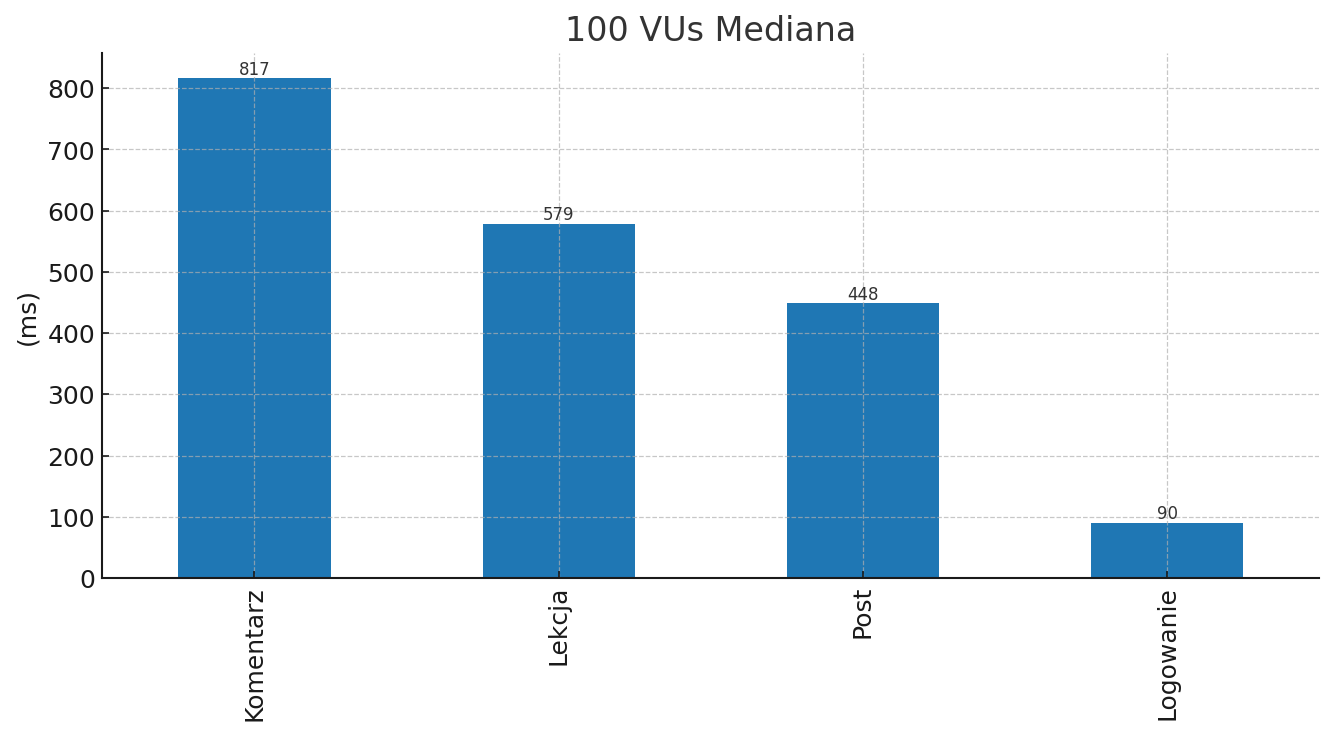
\includegraphics[width=\textwidth]{Dyplom-styl/chart_simple_100VU_mediana.png} \caption{100 VUs --- Mediana (ms). Źródło: Opracowanie własne}\label{fig:100-mediana} \end{figure} Mediany są niskie dla wszystkich operacji, operacje utrzymują komfortowy poziom opóźnień. \begin{figure}[H]\centering 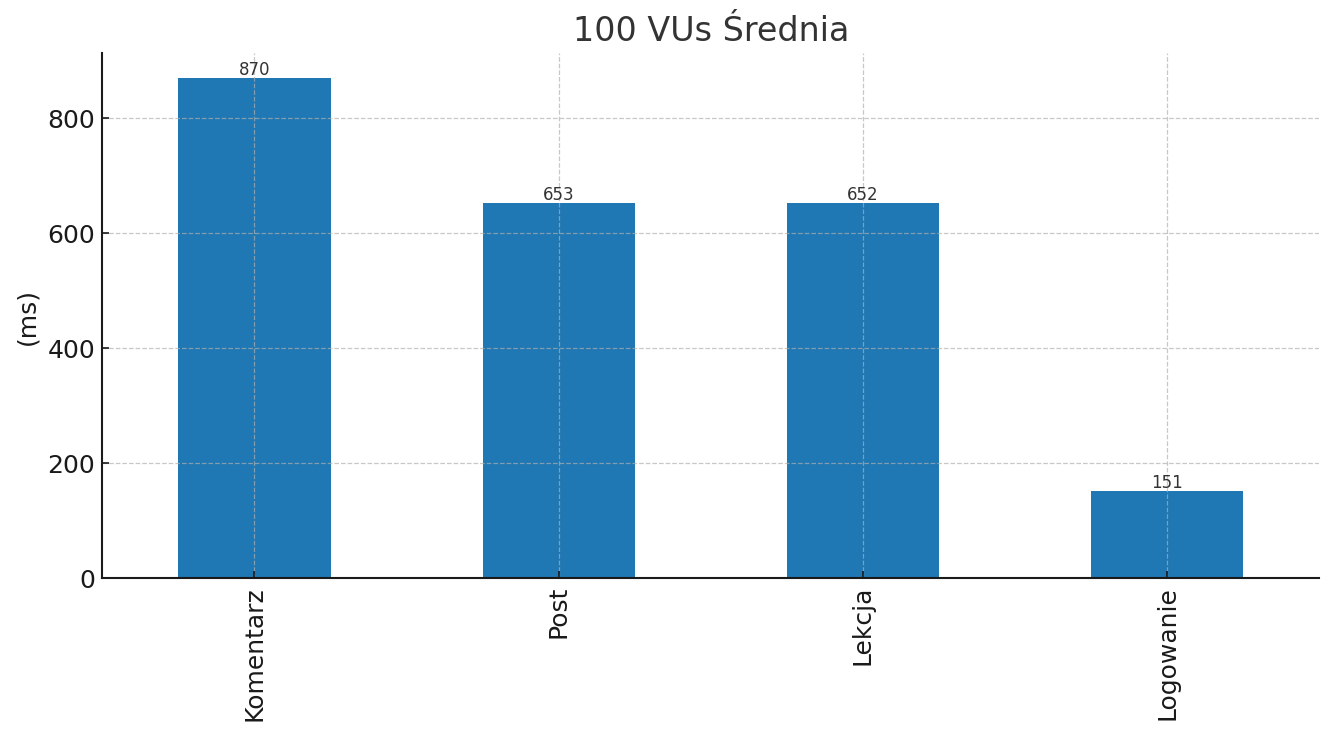
\includegraphics[width=\textwidth]{Dyplom-styl/chart_simple_100VU_srednia.png} \caption{100 VUs --- Średnia (ms). Źródło: Opracowanie własne}\label{fig:100-srednia} \end{figure} Średnie są zbliżone do median, co potwierdza stabilny profil obciążeń bez odchyleń. \begin{figure}[H]\centering 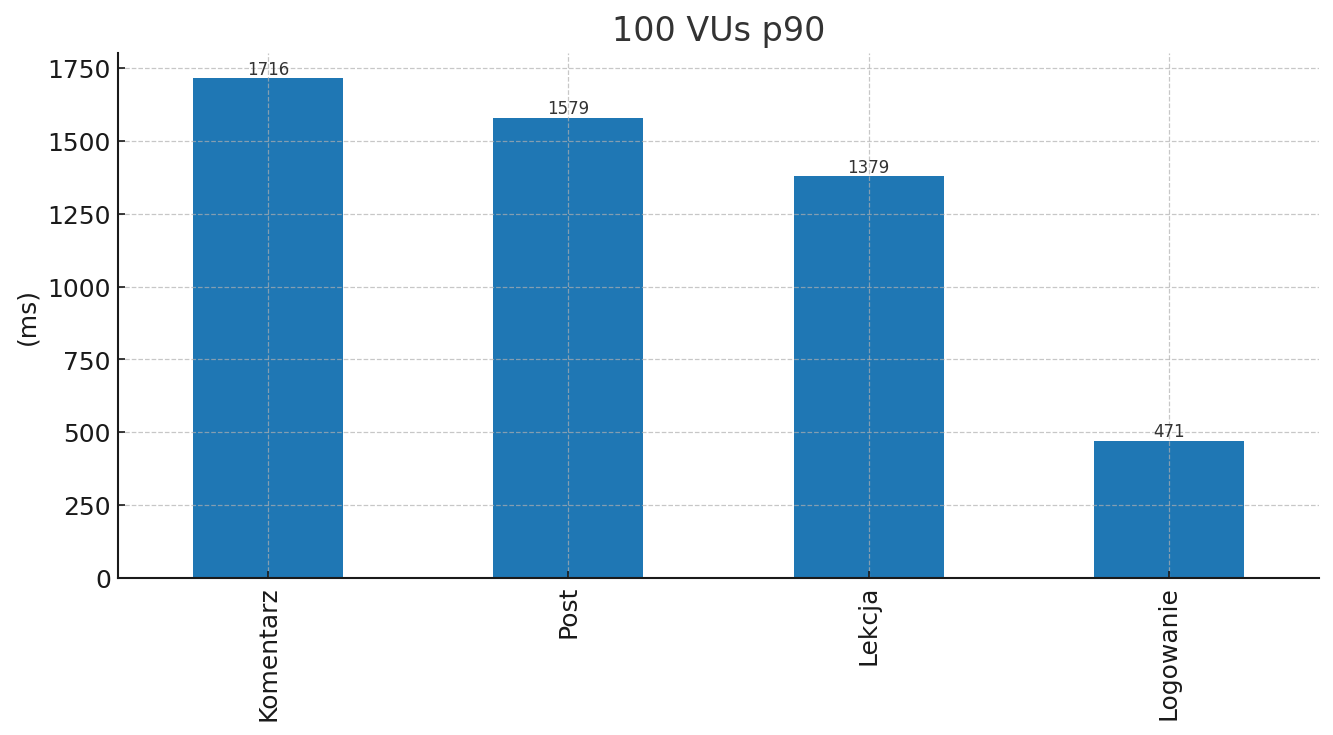
\includegraphics[width=\textwidth]{Dyplom-styl/chart_simple_100VU_p90.png} \caption{100 VUs --- p90 (ms). Źródło: Opracowanie własne}\label{fig:100-p90} \end{figure} p90 utrzymuje bezpieczny dystans od median, rezerwa wydajności jest wyraźna. \begin{figure}[H]\centering 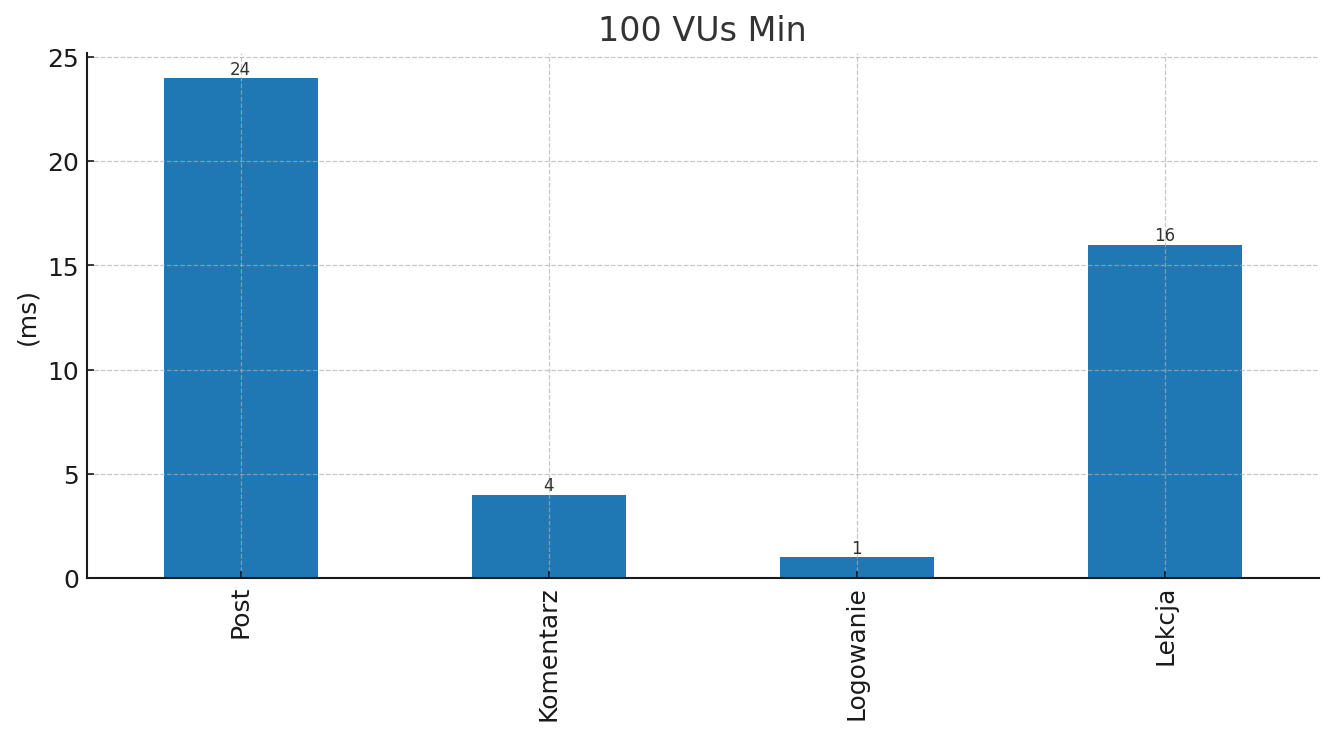
\includegraphics[width=\textwidth]{Dyplom-styl/chart_100VU_min_clean.png} \caption{100 VUs --- Min (ms). Źródło: Opracowanie własne }\label{fig:100-min} \end{figure} Minimalne czasy potwierdzają niskie koszty, żądań i szybką obsługę w pamięci.
\begin{figure}[H]\centering 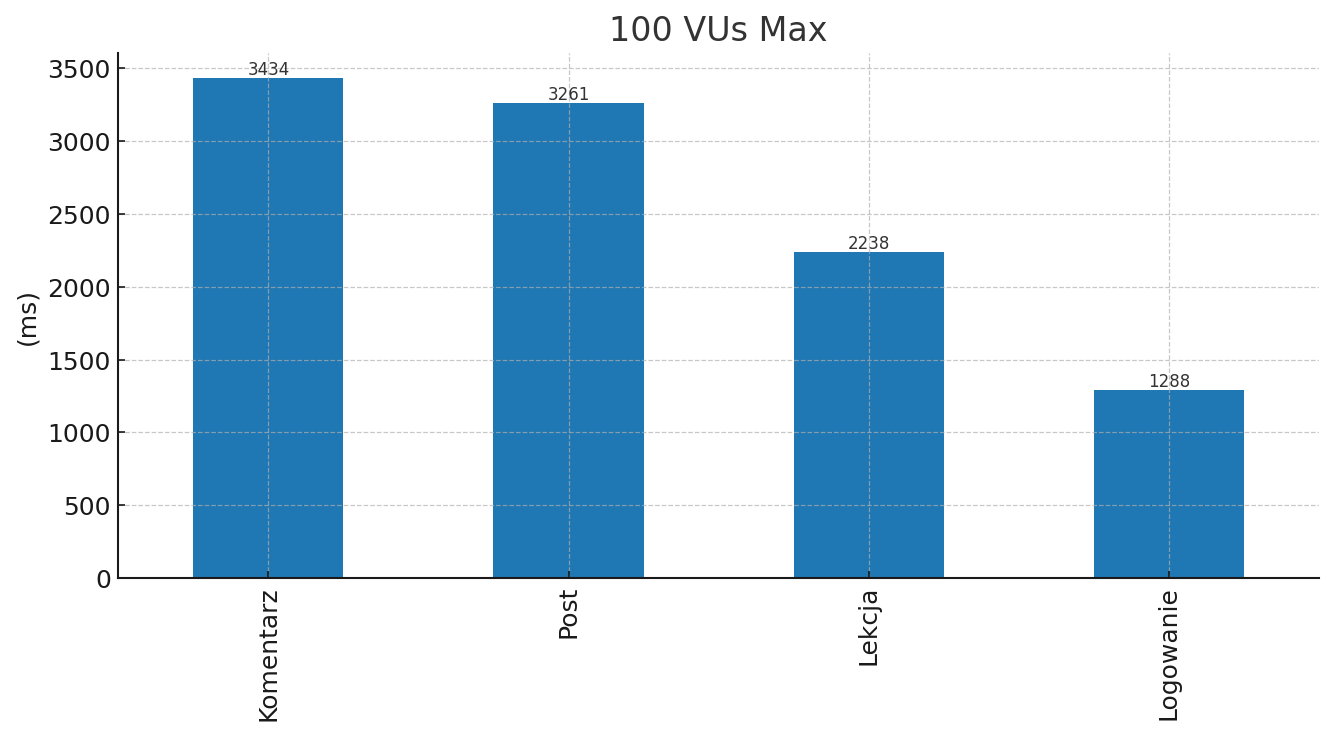
\includegraphics[width=\textwidth]{Dyplom-styl/chart_simple_100VU_max.png} \caption{100 VUs --- Max (ms). Źródło: Opracowanie własne }\label{fig:100-min} \end{figure} Maksymalne wartości występują okazjonalnie nie wpływając na odczucie podczas używania aplikacji.
% ===================== 250 VUs =====================
\subsubsection{250 VUs}

\begin{figure}[H]\centering
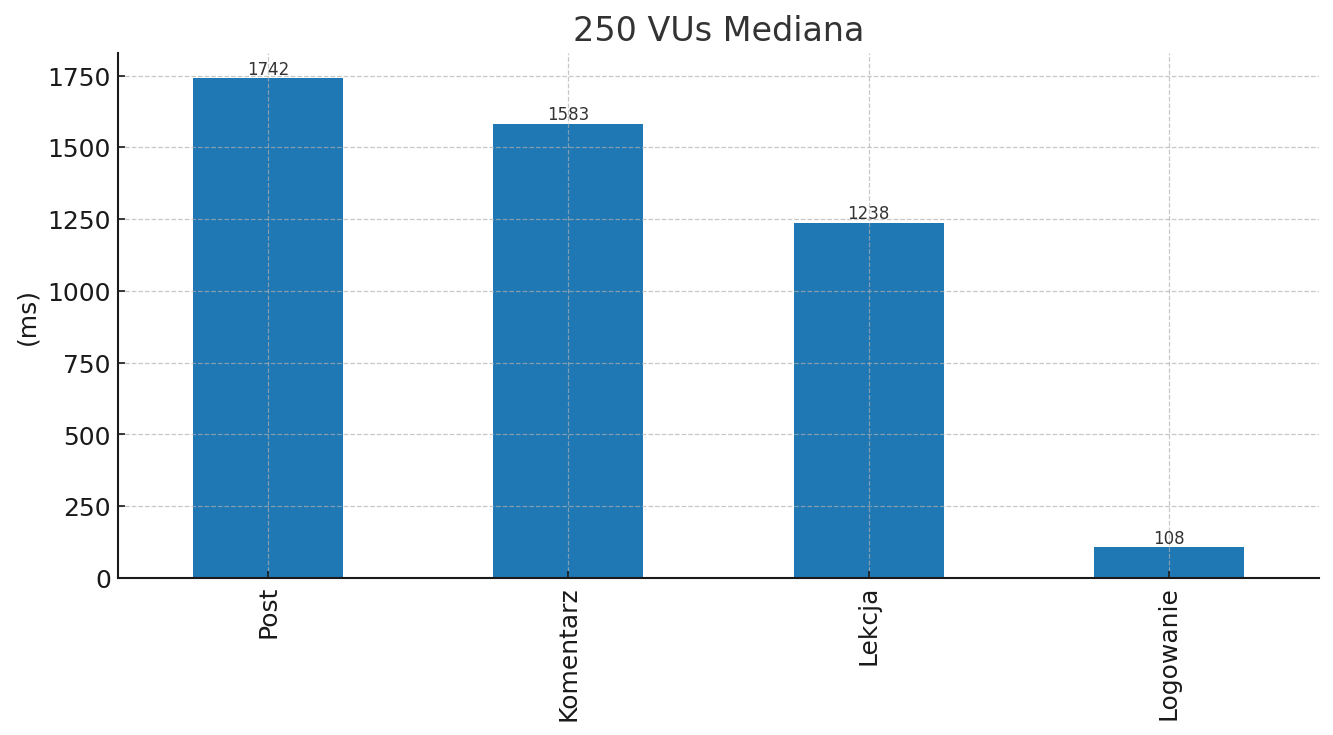
\includegraphics[width=\textwidth]{Dyplom-styl/chart_250VU_mediana.png}
\caption{250 VUs --- Mediana (ms). Źródło: Opracowanie własne}\label{fig:250-mediana}
\end{figure}
Wzrost obciążenia skutkuje przewidywalnym, łagodnym wzrostem median, brak skoków.

\begin{figure}[H]\centering
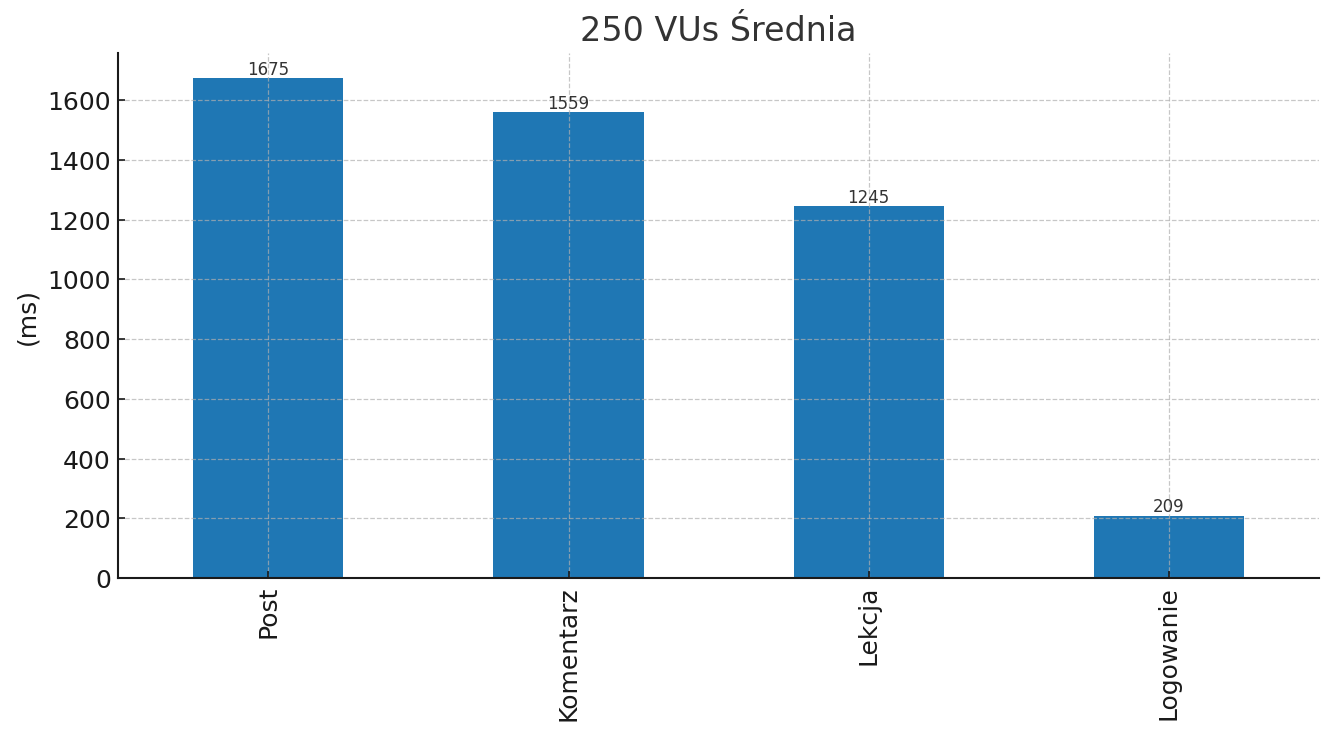
\includegraphics[width=\textwidth]{Dyplom-styl/chart_250VU_srednia.png}
\caption{250 VUs --- Średnia (ms). Źródło: Opracowanie własne}\label{fig:250-srednia}
\end{figure}
Średnie pomiarów pozostają w okolicy median, co potwierdza równomierny rozkład opóźnień.

\begin{figure}[H]\centering
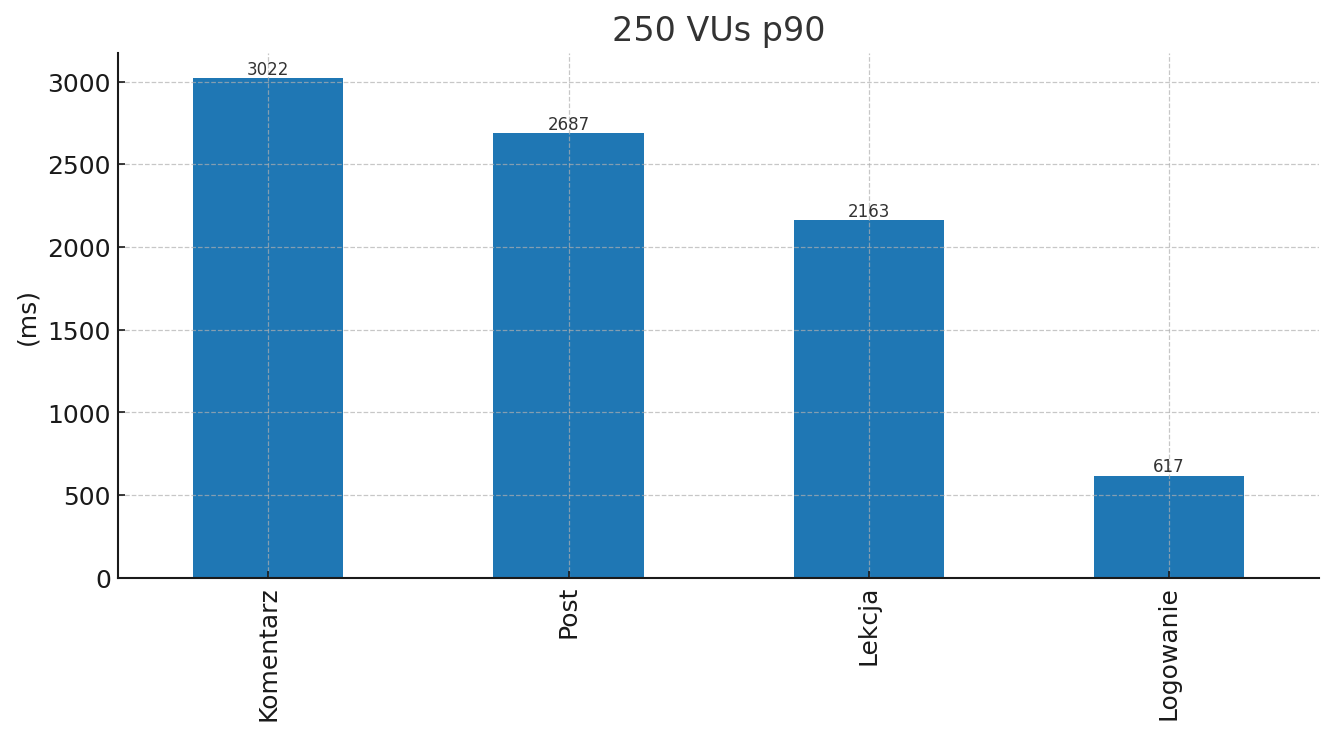
\includegraphics[width=\textwidth]{Dyplom-styl/chart_250VU_p90.png}
\caption{250 VUs --- p90 (ms). Źródło: Opracowanie własne}\label{fig:250-p90}
\end{figure}
p90 rośnie proporcjonalnie do obciążenia, utrzymując komfortowy zapas względem median.

\begin{figure}[H]\centering
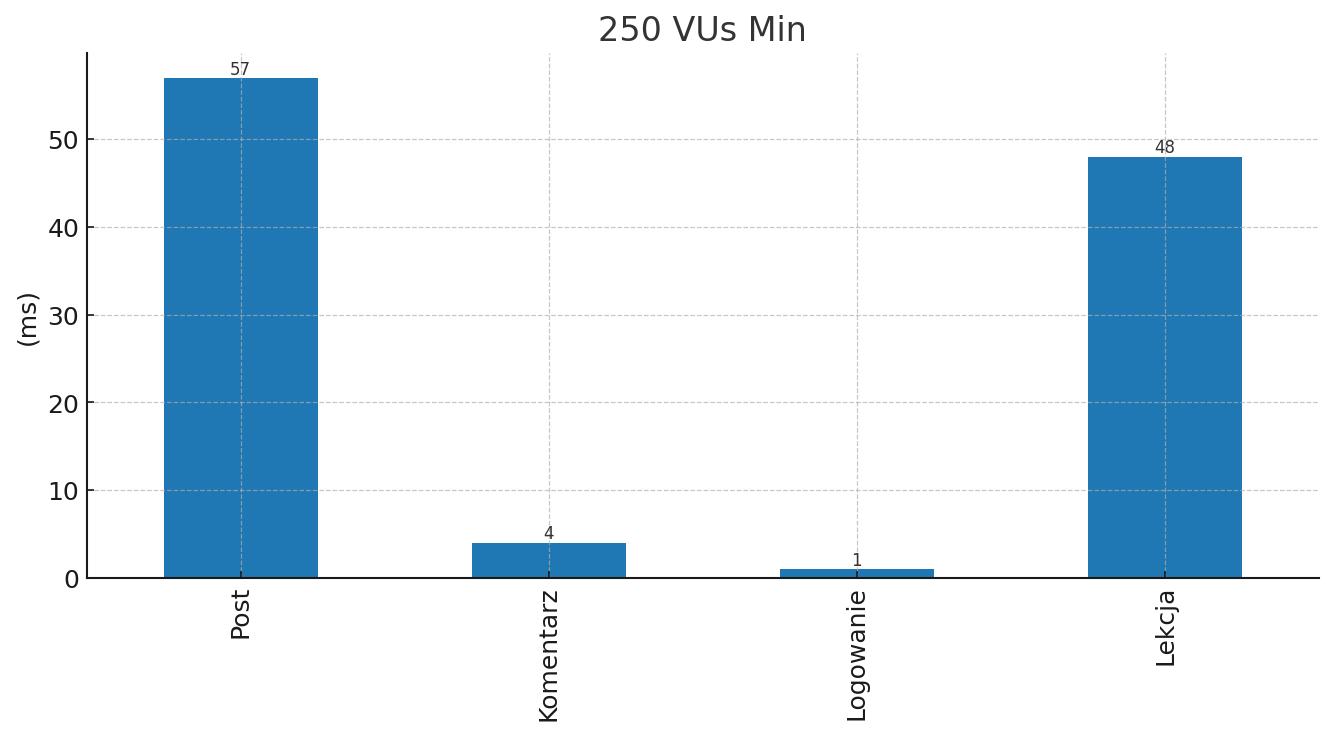
\includegraphics[width=\textwidth]{Dyplom-styl/chart_250VU_min_clean.png}
\caption{250 VUs --- Min (ms). Źródło: Opracowanie własne}\label{fig:250-min}
\end{figure}
Minimalne czasy pozostają bardzo niskie.

\begin{figure}[H]\centering
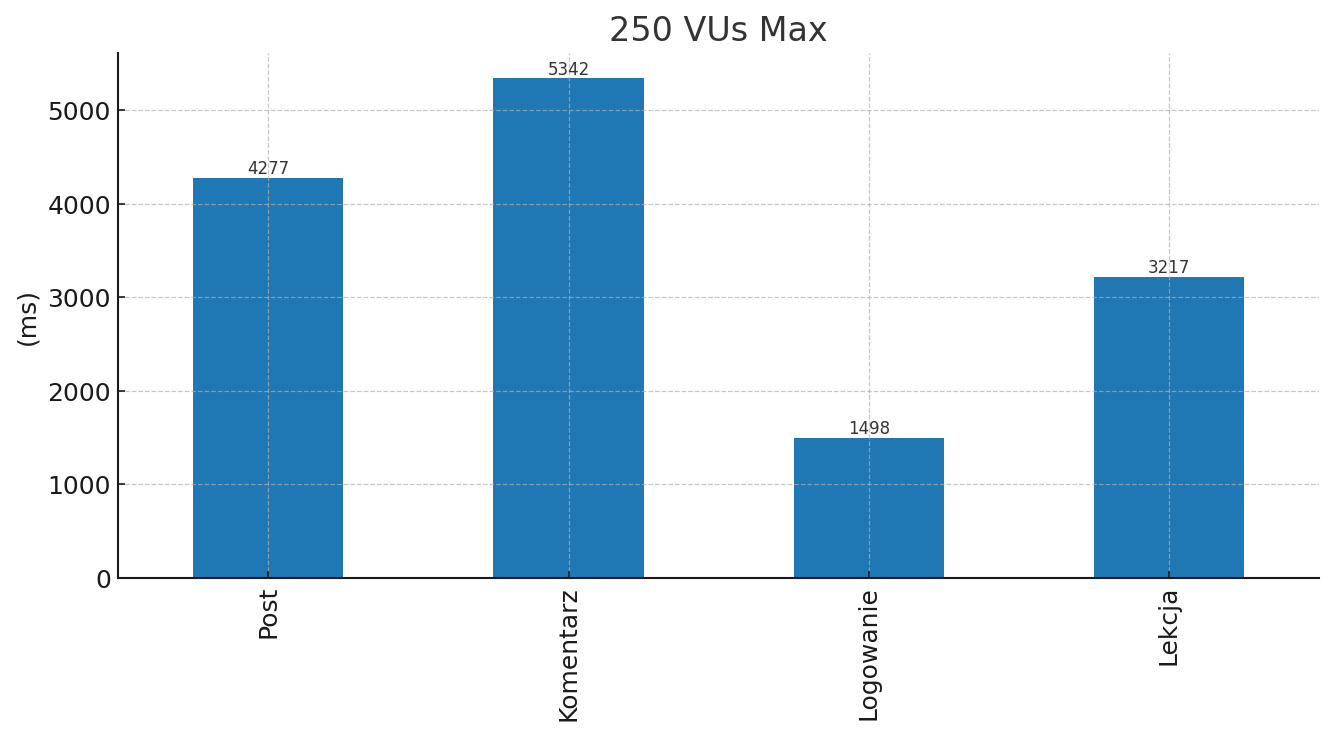
\includegraphics[width=\textwidth]{Dyplom-styl/chart_250VU_max_all4.png}
\caption{250 VUs --- Max (ms). Źródło: Opracowanie własne}\label{fig:250-max}
\end{figure}
Okazjonalne wartości szczytowe są pojedyncze i nie determinują ogólnego odczucia szybkości.

% ===================== 600 VUs =====================
\subsubsection{600 VUs}

\begin{figure}[H]\centering
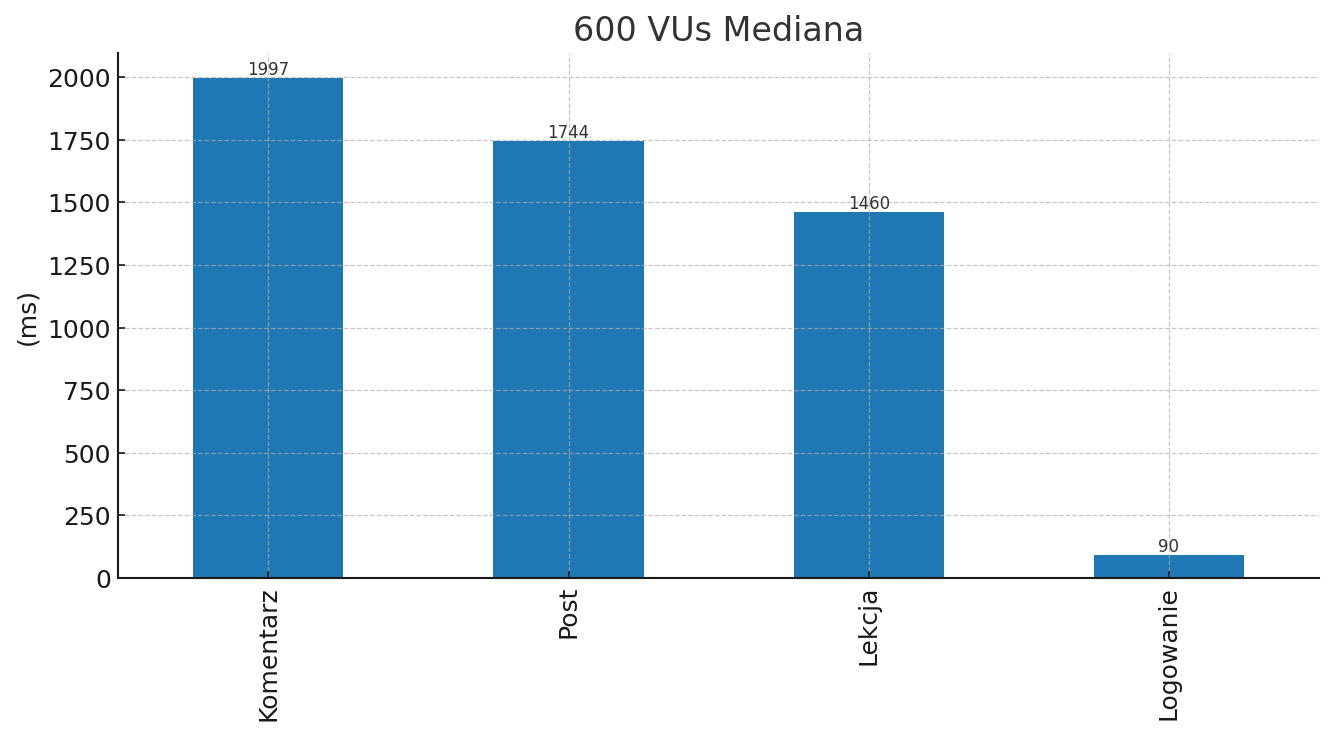
\includegraphics[width=\textwidth]{Dyplom-styl/chart_600VU_mediana.png}
\caption{600 VUs --- Mediana (ms). Źródło: Opracowanie własne}\label{fig:600-mediana}
\end{figure}
System skaluje się harmonijnie, mediany rosną łagodnie.

\begin{figure}[H]\centering
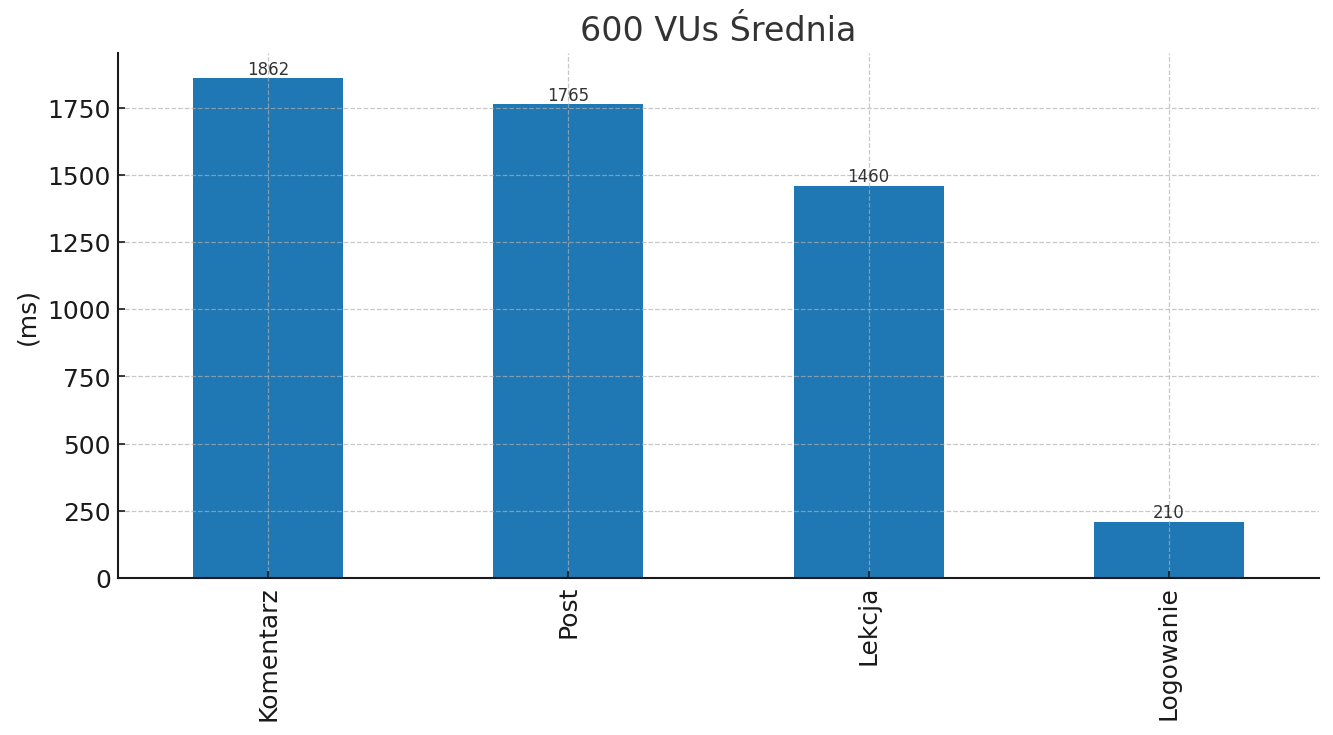
\includegraphics[width=\textwidth]{Dyplom-styl/chart_600VU_srednia.png}
\caption{600 VUs --- Średnia (ms). Źródło: Opracowanie własne}\label{fig:600-srednia}
\end{figure}
Średnie potwierdzają stabilność, opóźnienia pozostają przewidywalne.

\begin{figure}[H]\centering
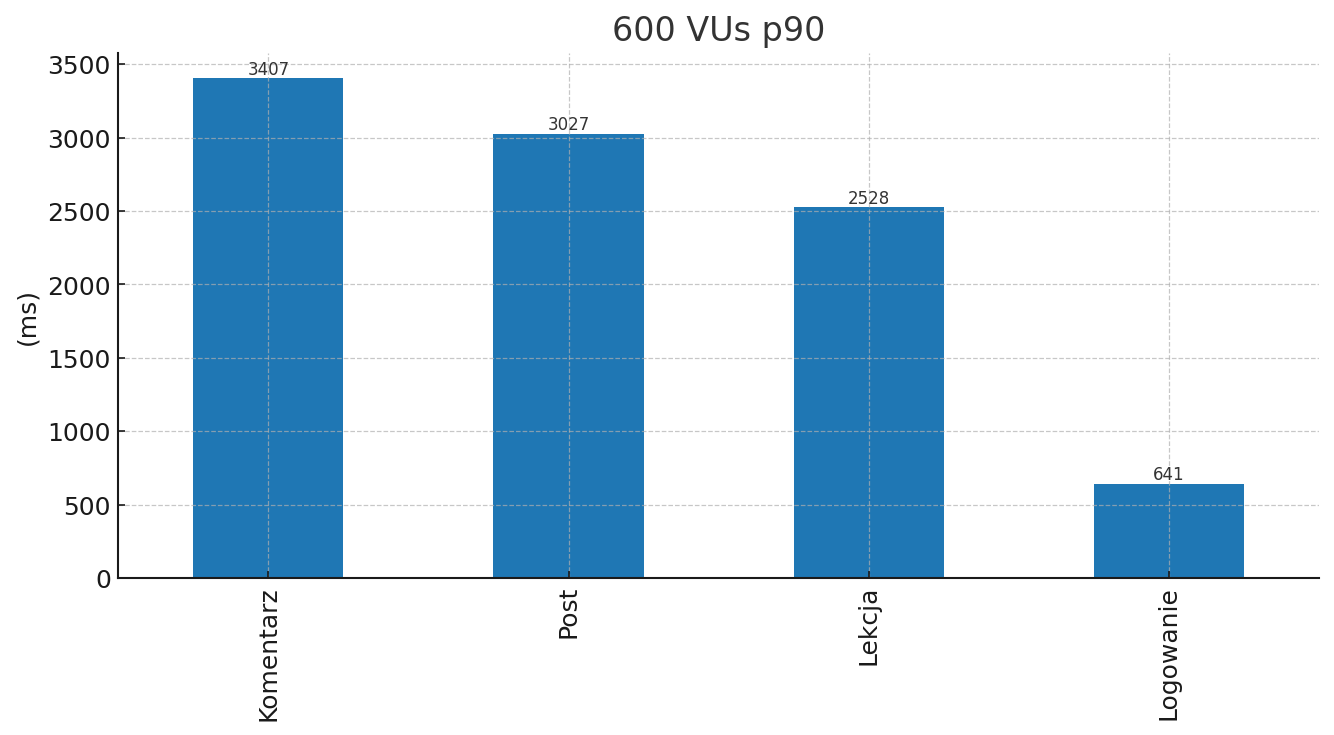
\includegraphics[width=\textwidth]{Dyplom-styl/chart_600VU_p90.png}
\caption{600 VUs --- p90 (ms). Źródło: Opracowanie własne}\label{fig:600-p90}
\end{figure}
p90 utrzymuje klarowną separację od median, co zapewnia komfort użytkownika także przy wyższych obciążeniach.

\begin{figure}[H]\centering
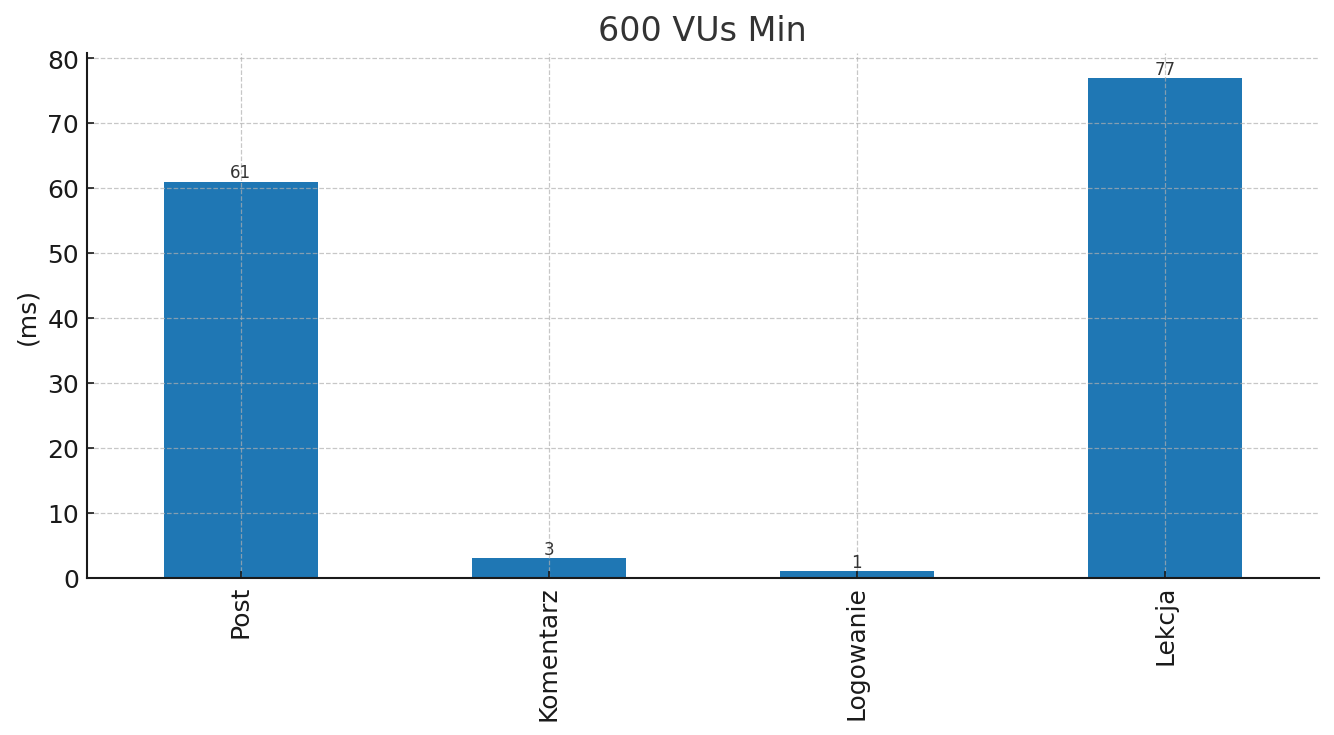
\includegraphics[width=\textwidth]{Dyplom-styl/chart_600VU_min_clean.png}
\caption{600 VUs --- Min (ms). Źródło: Opracowanie własne}\label{fig:600-min}
\end{figure}
Najniższe czasy nie ulegają pogorszeniu.

\begin{figure}[H]\centering
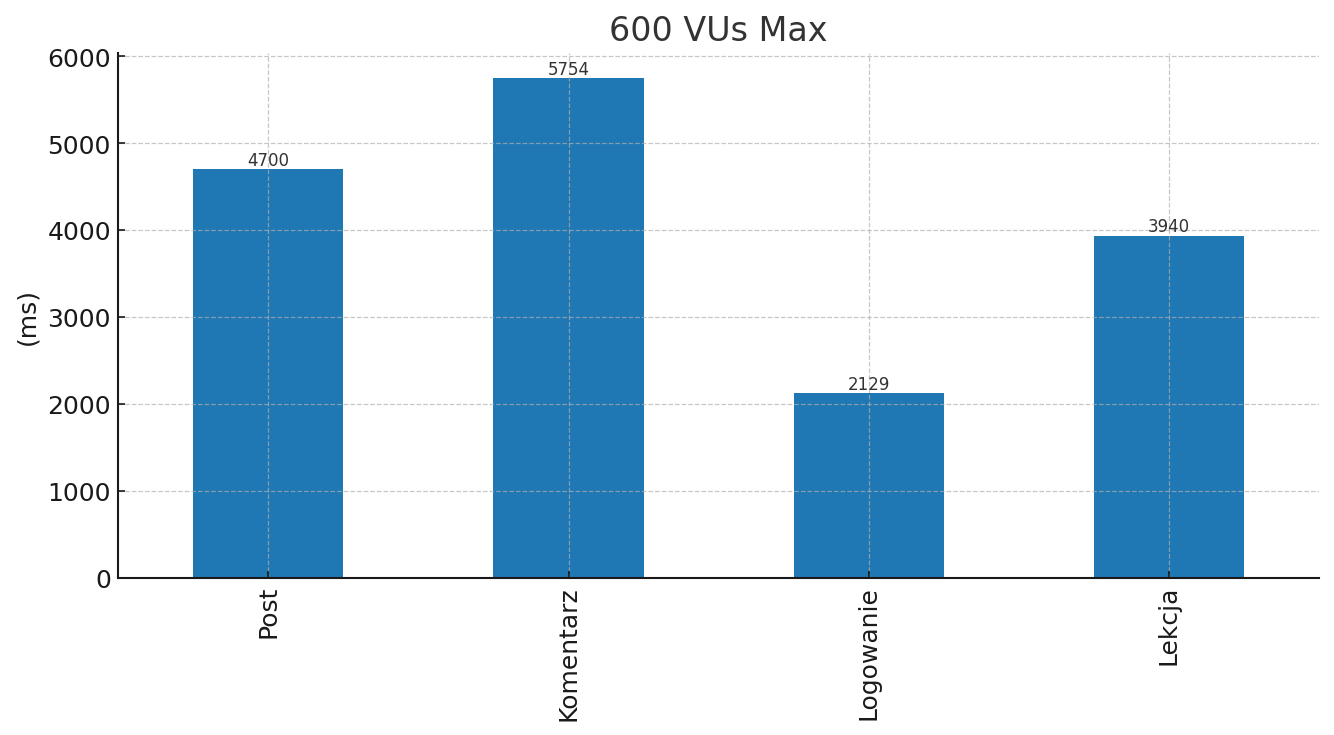
\includegraphics[width=\textwidth]{Dyplom-styl/chart_600VU_max_all4.png}
\caption{600 VUs --- Max (ms). Źródło: Opracowanie własne}\label{fig:600-max}
\end{figure}
Maksymalne wartości nadal pozostają w granicach komfortowego użytkowania.

% ===================== 1000 VUs =====================
\subsubsection{1000 VUs}

\begin{figure}[H]\centering
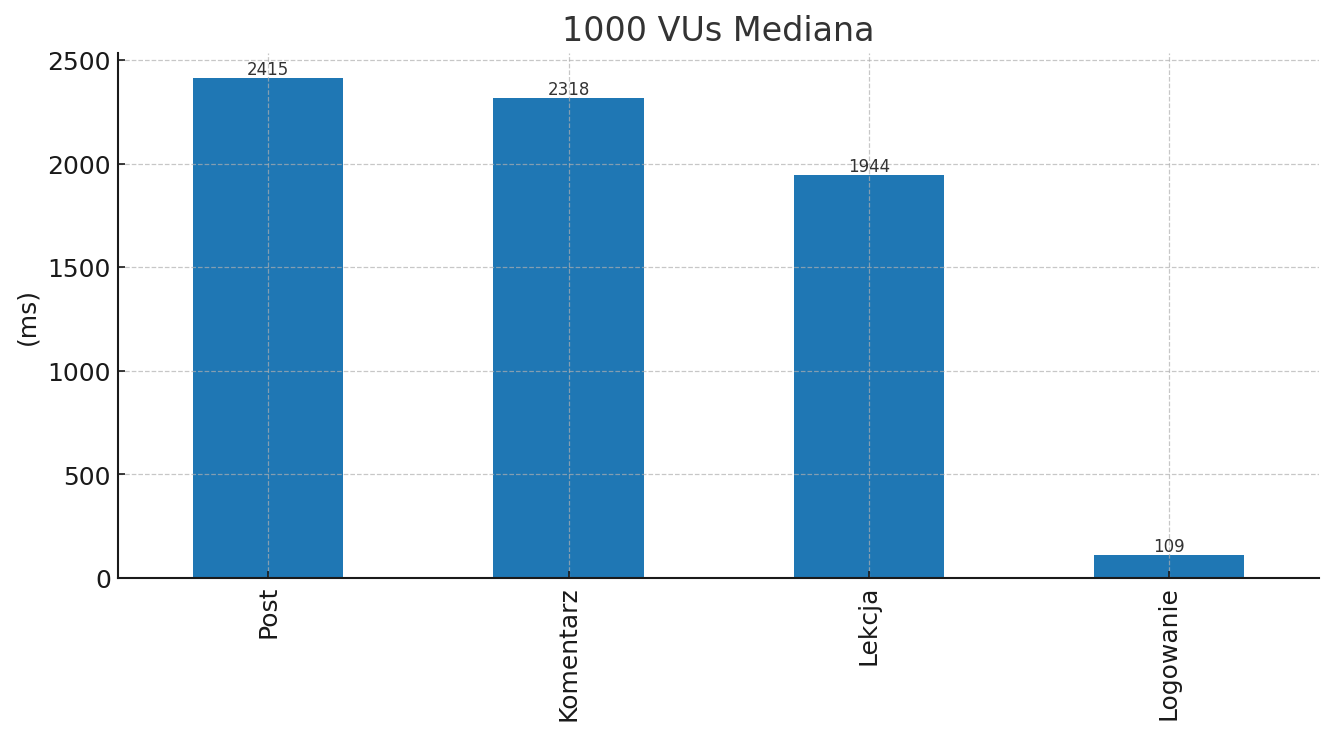
\includegraphics[width=\textwidth]{Dyplom-styl/chart_1000VU_mediana.png}
\caption{1000 VUs --- Mediana (ms). Źródło: Opracowanie własne}\label{fig:1000-mediana}
\end{figure}
Przy 1000 VUs mediany są nadal niskie, aplikacja zachowuje responsywność i płynność pracy.

\begin{figure}[H]\centering
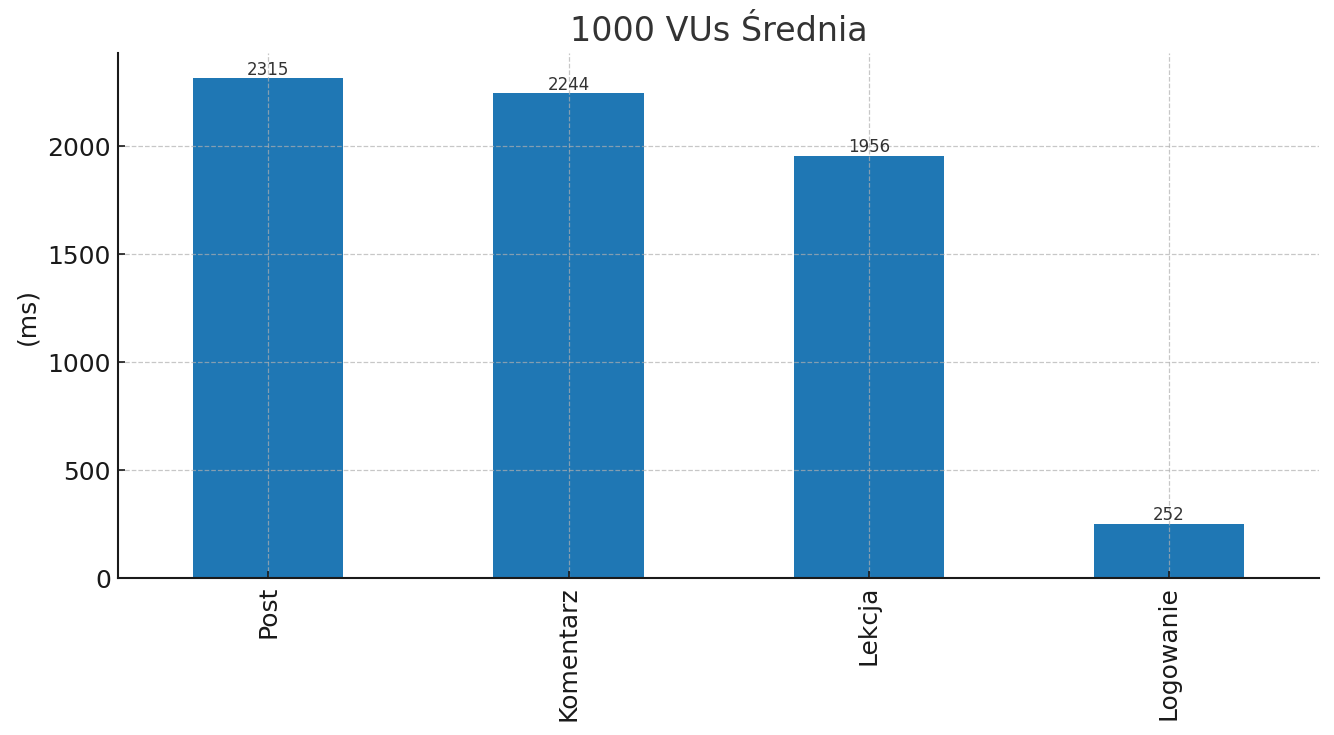
\includegraphics[width=\textwidth]{Dyplom-styl/chart_1000VU_srednia.png}
\caption{1000 VUs --- Średnia (ms). Źródło: Opracowanie własne}\label{fig:1000-srednia}
\end{figure}
Średnie czasy potwierdzają stabilność, widoczna jest spójność wyników.

\begin{figure}[H]\centering
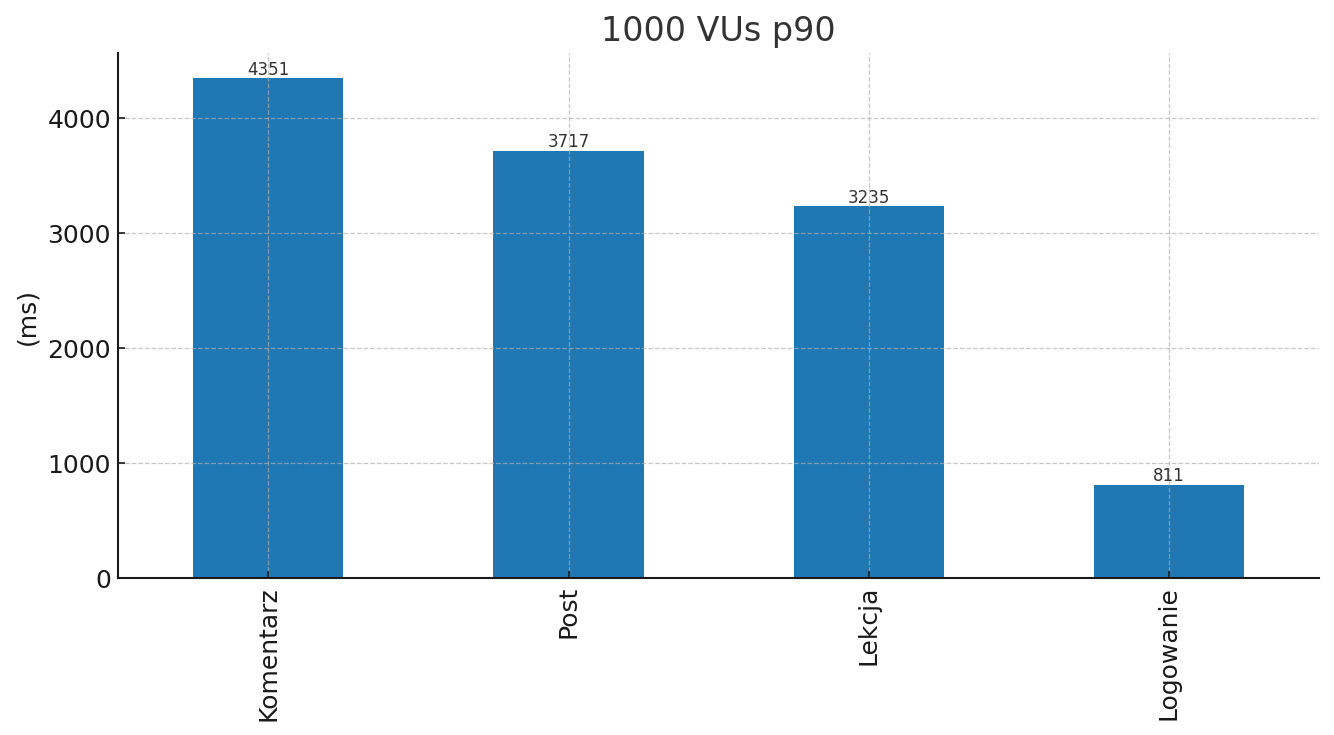
\includegraphics[width=\textwidth]{Dyplom-styl/chart_1000VU_p90.png}
\caption{1000 VUs --- p90 (ms). Źródło: Opracowanie własne}\label{fig:1000-p90}
\end{figure}
p90 pozostaje w rozsądnym zakresie, co gwarantuje komfortowe użytkowanie.

\begin{figure}[H]\centering
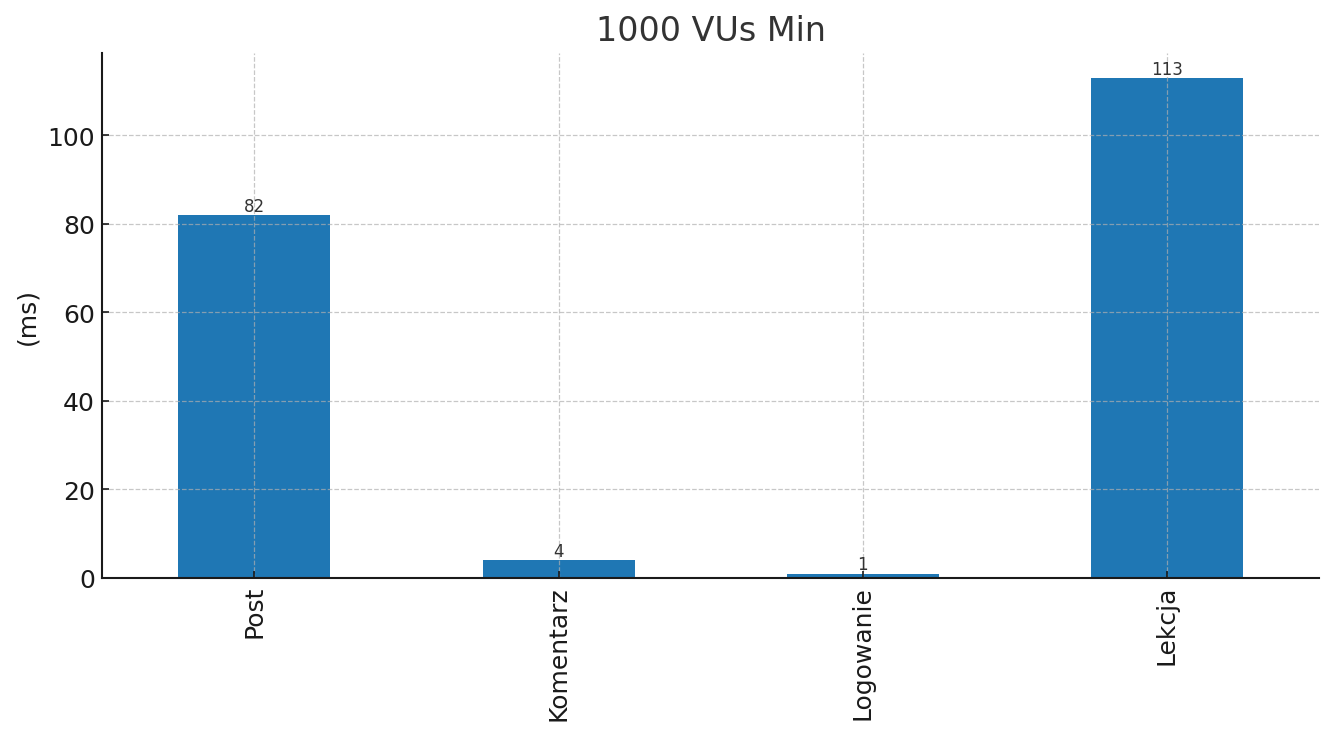
\includegraphics[width=\textwidth]{Dyplom-styl/chart_1000VU_min_clean.png}
\caption{1000 VUs --- Min (ms). Źródło: Opracowanie własne}\label{fig:1000-min}
\end{figure}
Minimalne czasy są bardzo niskie, przepływ żądań/zapytań jest efektywny.

\begin{figure}[H]\centering
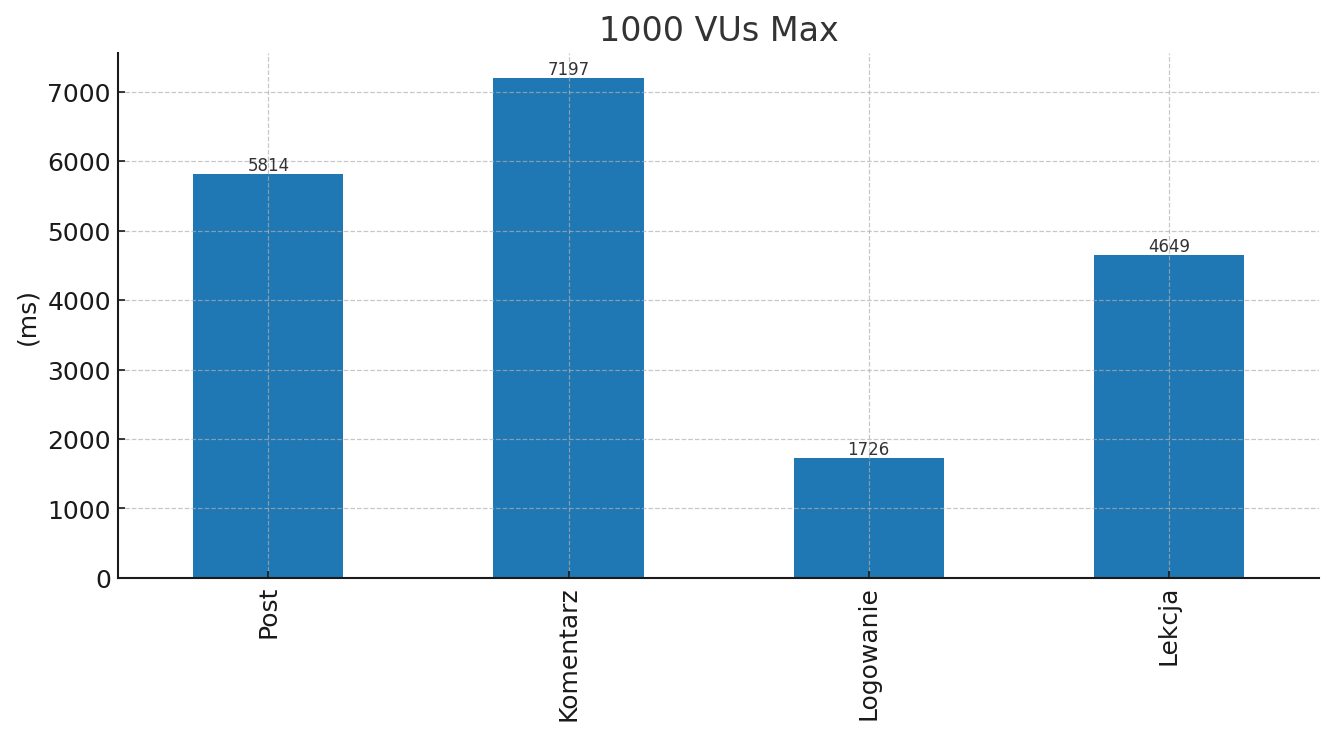
\includegraphics[width=\textwidth]{Dyplom-styl/chart_1000VU_max_all4.png}
\caption{1000 VUs --- Max (ms). Źródło: Opracowanie własne}\label{fig:1000-max}
\end{figure}
%\FloatBarrier 
Wartości maksymalne zachowują akceptowalny poziom, brak symptomów przeciążenia.
\subsection{podsumowanie wyników na wykresach liniowych}

\begin{figure}[H]\centering
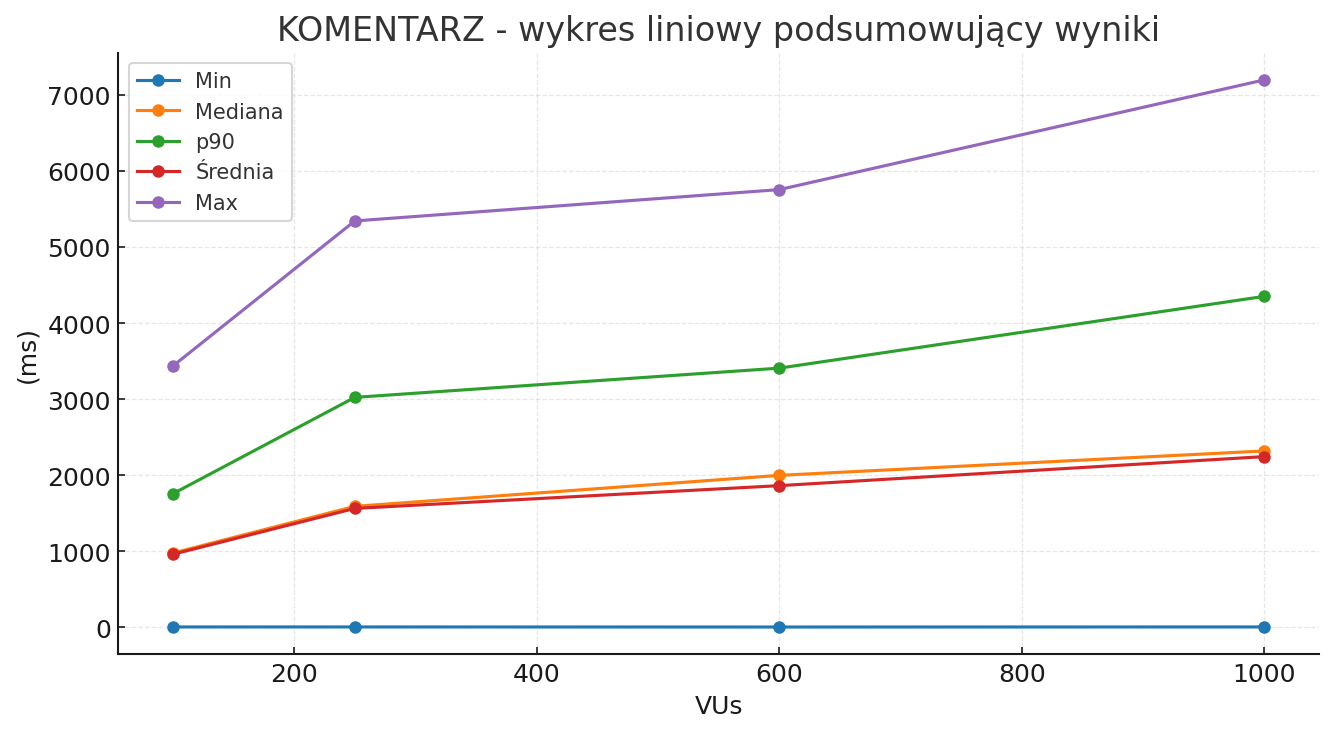
\includegraphics[width=\textwidth]{Dyplom-styl/line_komentarz_summary.png}
\caption{komentarz - wykres liniowy podsumowujący wyniki. Źródło: Opracowanie własne}\label{fig:line-post-summary}
\end{figure}
Trendy rosną łagodnie wraz z liczbą VU, operacja pozostaje responsywna podczas trwania testów.

\begin{figure}[H]\centering
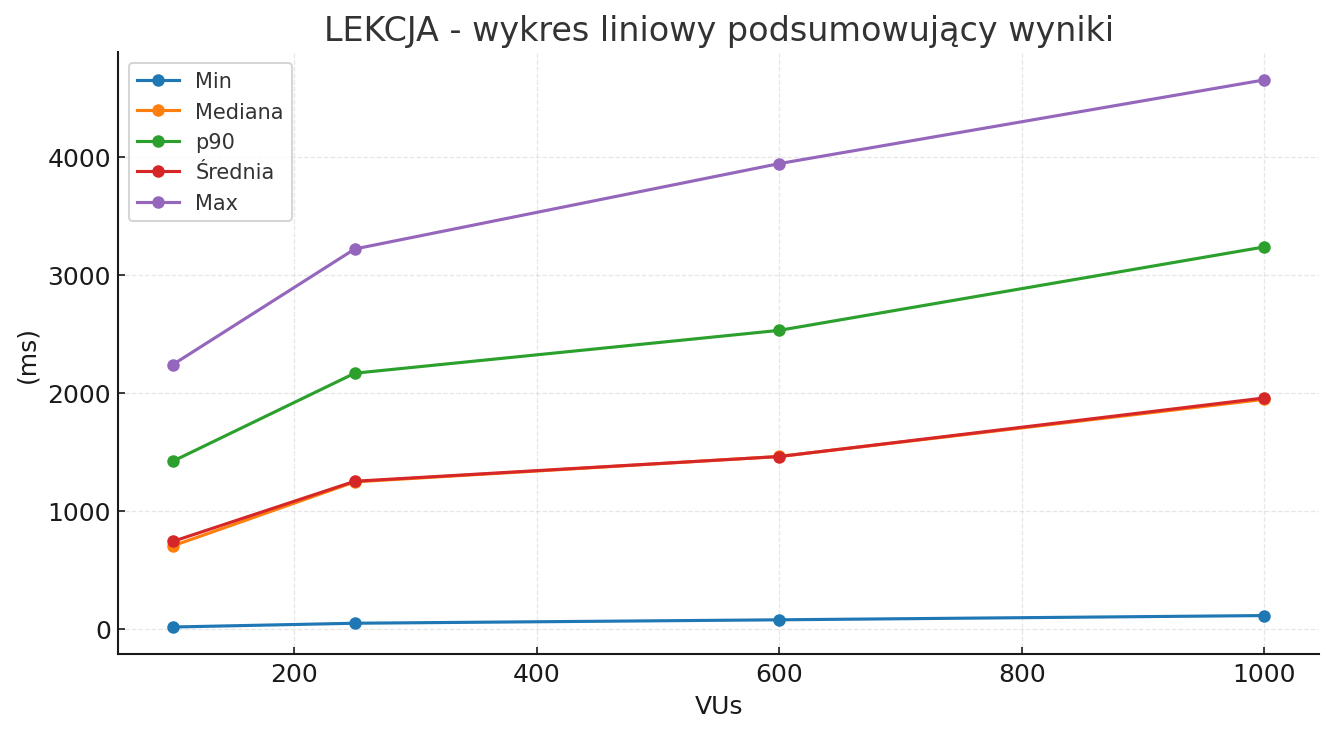
\includegraphics[width=\textwidth]{Dyplom-styl/line_lekcja_summary.png}
\caption{dodanie komentarza — wykres liniowy podsumowujący wyniki. Źródło: Opracowanie własne}\label{fig:line-komentarz-summary}
\end{figure}
Stabilny wzrost metryk wraz z VU bez skokowych zmian, p90 pozostaje pod kontrolą, a operacja skaluje się przewidywalnie.

\begin{figure}[H]\centering
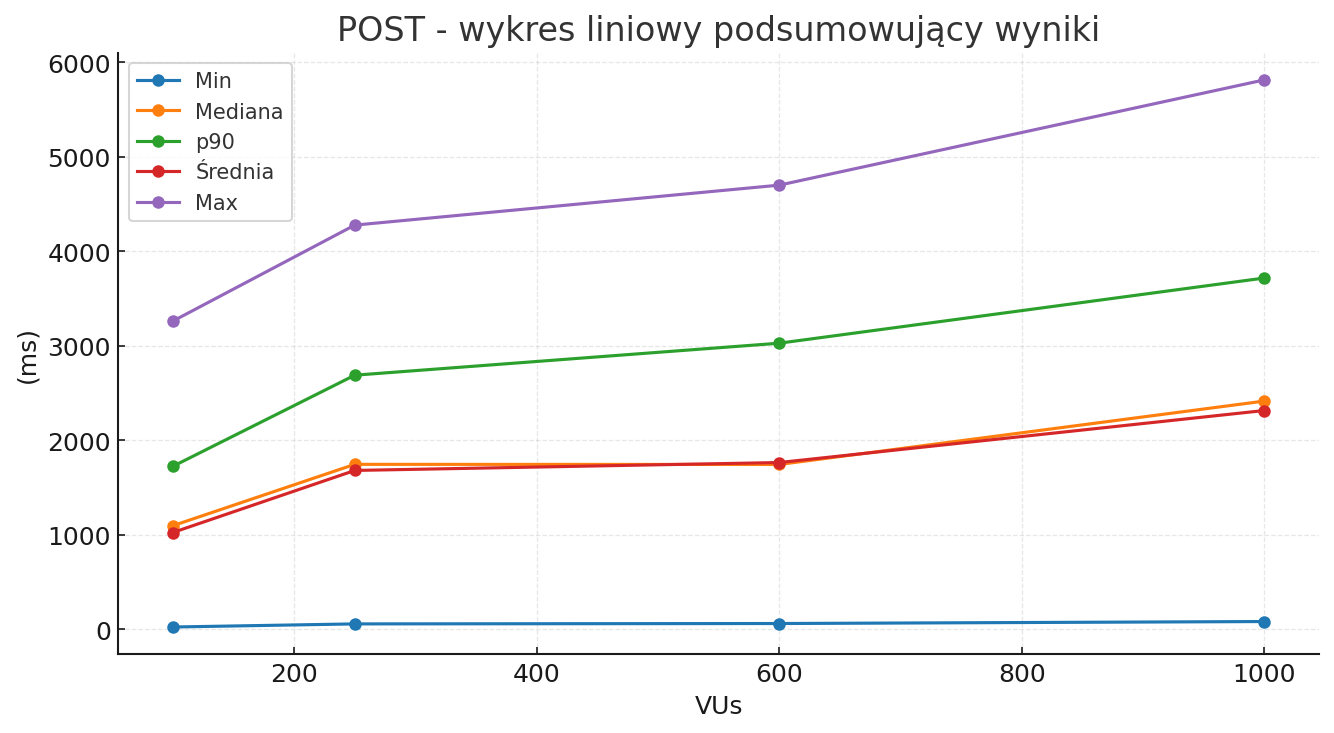
\includegraphics[width=\textwidth]{Dyplom-styl/line_post_summary.png}
\caption{dodanie "post" — wykres liniowy podsumowujący wyniki. Źródło: Opracowanie własne}\label{fig:line-post-summary}
\end{figure}
Czasy rosną proporcjonalnie do VU, p90 pozostaje blisko mediany, co potwierdza stabilne zachowanie pod obciążeniem.

\begin{figure}[H]\centering
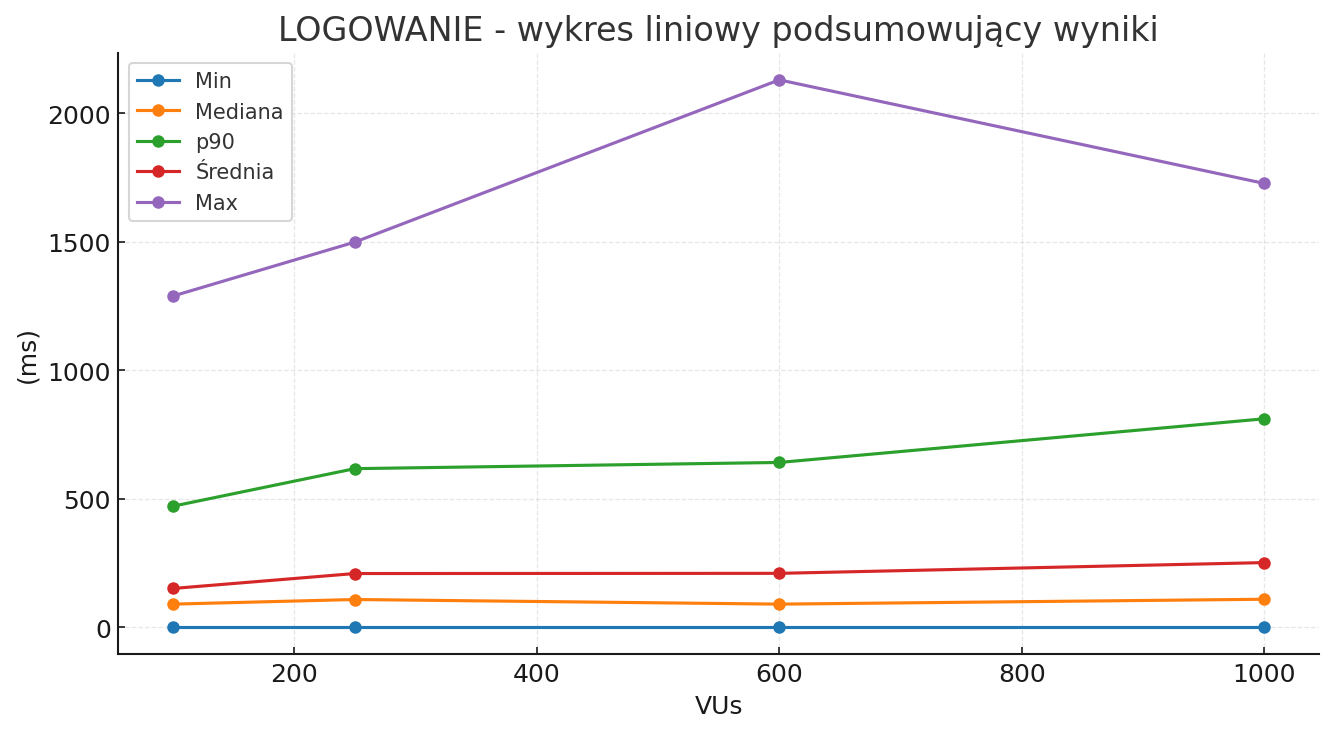
\includegraphics[width=\textwidth]{Dyplom-styl/line_logowanie_summary.png}
\caption{logowanie — wykres liniowy podsumowujący wyniki. Źródło: Opracowanie własne}\label{fig:line-logowanie-summary}
\end{figure}
Najkrótsze czasy w całej próbie, nawet przy 1000 VUs utrzymana niska mediana i p90, co zapewnia bardzo dobrą responsywność.
\FloatBarrier 

\subsection{Podsumowanie wyników w tabelach}

\begingroup
  \let\oldcaption\caption
  \renewcommand{\caption}[2][]{\oldcaption[#1]{#2. Źródło: opracowanie własne}}
  \begin{table}[H]
\centering
\caption{Mediana czasu odpowiedzi (ms) — wiersze: VUs, kolumny: endpoint}
\label{tab:mediana-vs-vus}
\begin{tabular}{rrrrr}
\toprule
 VUs &   Post &  Komentarz &  Logowanie &  Lekcja \\
\midrule
 100 & 1096.0 &      975.0 &       90.0 &   703.0 \\
 250 & 1745.5 &     1589.5 &      108.0 &  1245.0 \\
 600 & 1744.0 &     1997.0 &       90.0 &  1460.0 \\
1000 & 2415.0 &     2318.0 &      109.0 &  1944.0 \\
\bottomrule
\end{tabular}
\end{table}

\endgroup
Mediany rosną proporcjonalnie do VUs, z zachowaniem niskich wartości i czytelnej przewagi logowania.

\begingroup
  \let\oldcaption\caption
  \renewcommand{\caption}[2][]{\oldcaption[#1]{#2. Źródło: opracowanie własne}}
  \begin{table}[H]
\centering
\caption{Średni czas czasu odpowiedzi (ms) — wiersze: VUs, kolumny: endpoint}
\label{tab:srednia-vs-vus}
\begin{tabular}{rrrrr}
\toprule
 VUs &        Post &   Komentarz &  Logowanie &      Lekcja \\
\midrule
 100 & 1024.152679 &  959.206359 &   150.8700 &  740.664055 \\
 250 & 1680.865622 & 1562.238743 &   209.0150 & 1250.261864 \\
 600 & 1764.604294 & 1861.691186 &   209.7275 & 1459.649407 \\
1000 & 2315.134783 & 2243.617152 &   251.5425 & 1955.728077 \\
\bottomrule
\end{tabular}
\end{table}

\endgroup
Średnie pokrywają się z trendem median, wyniki są spójne między operacjami.

\begingroup
  \let\oldcaption\caption
  \renewcommand{\caption}[2][]{\oldcaption[#1]{#2. Źródło: opracowanie własne}}
  \begin{table}[H]
\centering
\caption{p90 czasu odpowiedzi (ms) — wiersze: VUs, kolumny: endpoint}
\label{tab:p90-vs-vus}
\begin{tabular}{rrrrr}
\toprule
 VUs &   Post &  Komentarz &  Logowanie &  Lekcja \\
\midrule
 100 & 1724.3 &     1755.0 &      470.8 &  1420.0 \\
 250 & 2688.8 &     3022.2 &      616.9 &  2165.1 \\
 600 & 3027.5 &     3406.8 &      641.0 &  2528.0 \\
1000 & 3717.2 &     4350.7 &      810.9 &  3234.7 \\
\bottomrule
\end{tabular}
\end{table}

\endgroup
p90 pozostaje przewidywalnie wyższy od median, ale utrzymuje komfortowe zakresy.

\begingroup
  \let\oldcaption\caption
  \renewcommand{\caption}[2][]{\oldcaption[#1]{#2. Źródło: opracowanie własne}}
  \begin{table}[H]
\centering
\caption{Minimum czasu odpowiedzi (ms) — wiersze: VUs, kolumny: endpoint}
\label{tab:min-vs-vus}
\begin{tabular}{rrrrr}
\toprule
 VUs &  Post &  Komentarz &  Logowanie &  Lekcja \\
\midrule
 100 &    24 &          4 &          1 &      16 \\
 250 &    57 &          4 &          1 &      48 \\
 600 &    61 &          3 &          1 &      77 \\
1000 &    82 &          4 &          1 &     113 \\
\bottomrule
\end{tabular}
\end{table}

\endgroup
Minimalne czasy potwierdzają niski czas przetwarzania, ścieżki są zoptymalizowane.

\begingroup
  \let\oldcaption\caption
  \renewcommand{\caption}[2][]{\oldcaption[#1]{#2. Źródło: opracowanie własne}}
  \begin{table}[H]
\centering
\caption{Maksimum czasu odpowiedzi (ms) — wiersze: VUs, kolumny: endpoint}
\label{tab:max-vs-vus}
\begin{tabular}{rrrrr}
\toprule
 VUs &  Post &  Komentarz &  Logowanie &  Lekcja \\
\midrule
 100 &  3261 &       3434 &       1288 &    2238 \\
 250 &  4277 &       5342 &       1498 &    3217 \\
 600 &  4700 &       5754 &       2129 &    3940 \\
1000 &  5814 &       7197 &       1726 &    4649 \\
\bottomrule
\end{tabular}
\end{table}

\endgroup
Maksymalne wartości są pojedynczymi przypadkami i nie wpływają na ogólne odczucie podczas używania aplikacji.


\FloatBarrier


% ===================== Podsumowanie =====================
\subsection{Podsumowanie testów wydajnościowych i jakościowych}

Przeprowadzony zestaw testów obejmował trzy komplementarne poziomy jakości:
\textbf{(1) testy jednostkowe} logiki domenowej (w tym serwisy, walidacja, operacje na repozytoriach Hazelcast),
\textbf{(2) testy integracyjne end-to-end} z użyciem wbudowanego serwera i klienta HTTP,
oraz \textbf{(3) testy wydajnościowe} w JMeter \cite{jmeter-docs}.
Takie ułożenie testów pozwoliło jednocześnie weryfikować poprawność funkcjonalną
i obserwować zachowanie systemu pod obciążeniem.

\paragraph{Poprawność funkcjonalności (jednostkowe \& integracyjne).}
Testy jednostkowe potwierdziły spójność logiki serwisów oraz prawidłowość filtracji w bazie danych.
Testy integracyjne end-to-end odwzorowały typowe działania podejmowane przez użytkowników (logowanie, dodawanie treści, interakcje użytkownika),
wskazując na poprawną współpracę warstw (kontrolery~$\leftrightarrow$~serwisy~$\leftrightarrow$~baza danych) oraz
na prawidłową obsługę sesji i CSRF. Operacje CRUD przebiegały zgodnie z oczekiwaniami, a odpowiedzi HTTP
zwracały oczekiwane kody i treści.

\paragraph{Wydajność i skalowalność (100--1000 VU).}
W testach obciążeniowych zróżnicowano liczbę równoczesnych użytkowników (100, 250, 600, 1000 VUs),
co pozwoliło zbadać zachowanie systemu pod rosnącym obciążeniem bez wprowadzania długotrwałego stresu.
Zebrane metryki (Mediana, Średnia, p90, Min, Max) wskazują na:
\begin{itemize}
  \item \textbf{Stabilny wzrost opóźnień} wraz ze wzrostem obciążenia, mediany rosną powoli,
        a p90 pozostaje w dobrym odstępie od mediany (Rys. \ref{fig:line-post-summary}).
  \item \textbf{Najkrótsze czasy dla Logowania}, co jest spójne z charakterem operacji (niewielka ilość przesłanych i otrzymanych danych).
        Operacje dodanie Posta i Komentarza są nieco większe, ale utrzymują niskie mediany oraz korzystne p90.
  \item \textbf{Lekcja} (dodanie lekcji) prezentuje trend porównywalny z dodaniem posta, stabilny bez skokowych zmian.
  \item \textbf{wartości Minimalne} wartości minimalnego czasu odpowiedzi potwierdzają, że ścieżka przetwarzania jest zoptymalizowana.
\item \textbf{wartości maksymalne} występują  sporadycznie, i nie wpływają na komfort użytkowania aplikacji
        (mediana i p90 mają niskie wartości).
\end{itemize}

\paragraph{Odczyt wyników na wykresach i w tabelach.}
\emph{Wykresy liniowe per operacja} (np. Rys. \ref{fig:line-post-summary}) pokazują,
że dla całego zakresu 100--1000 VU zachowany jest przewidywalny trend i komfortowe czasy odpowiedzi
dla wszystkich pięciu metryk. Wykresy słupkowe dla poszczególnych obciążeń
konsekwentnie potwierdzają te obserwacje. Tabele:
\textbf{Median} (Tab.~\ref{tab:mediana-vs-vus}),
\textbf{Średnich wartości} (Tab.~\ref{tab:srednia-vs-vus}),
\textbf{p90} (Tab.~\ref{tab:p90-vs-vus}),
\textbf{Minimalnych wartości} (Tab.~\ref{tab:min-vs-vus}) i
\textbf{maksymalnych wartości} (Tab.~\ref{tab:max-vs-vus})
Tabele przedstawiają zbiorcze zestawienie wyników, w którym wiersze odpowiadają liczbie wirtualnych użytkowników (VUs), a kolumny – poszczególnym operacjom. Potwierdzają trendy z wykresów.

\paragraph{Wnioski techniczne.}
Zastosowanie Hazelcast jako bazy danych sprzyja niskim opóźnieniom i stałości czasów odpowiedzi,
co widać szczególnie po medianie i p90. Architektura aplikacji wykazuje dobrą skalowalność wertykalną. W testowanym zakresie obciążenia, wzrost liczby wirtualnych użytkowników (VUs) nie ujawnił wąskich gardeł ani punktów saturacji. Profile wydajnościowe poszczególnych operacji pozostają spójne, co stanowi solidną podstawę do skalowania horyzontalnego (poprzez dodawanie kolejnych instancji aplikacji i węzłów Hazelcast) z zachowaniem niskich czasów odpowiedzi \cite{microservices}.

\paragraph{Konkluzja.}
W świetle przeprowadzonych testów można stwierdzić że,
aplikacja jest funkcjonalnie poprawna i spójna,
wydajna i przewidywalna,
gotowa do skalowania wraz z rosnącym ruchem.
Uzyskane charakterystyki wskazują na dojrzałość rozwiązania i jego przydatność do obsługi
współbieżnego ruchu w kontekście udostępniania materiałów edukacyjnych. % chapter6.tex zawiera treść rozdziału 6


\chapter{Podsumowanie projektu i wnioski}
W ramach zrealizowanego projektu stworzono funkcjonalną platformę webową służącą do udostępniania materiałów edukacyjnych, zarządzania kursami oraz interakcji między studentami a nauczycielami. Aplikacja została zaprojektowana i wykonana w oparciu o nowoczesny stos technologiczny (Spring Boot 3, Java 23, Thymeleaf, Bootstrap) z nietypowym rozwiązaniem w zakresie przechowywania danych użyciem bazy danych w pamięci Hazelcast zamiast tradycyjnej bazy relacyjnej. W toku implementacji osiągnięto założone cele funkcjonalne: użytkownicy mogą się rejestrować i logować, nauczyciele tworzyć kursy i materiały, studenci zapisywać na zajęcia i przesyłać zadania, a administratorzy nadzorować całość systemu i analizować statystyki. Rezultatem prac jest prototyp platformy e-learningowej o prostej, przejrzystej obsłudze, który może stanowić podstawę do dalszego rozwoju lub wdrożenia na potrzeby uczelni czy kursów online. W trakcie testów potwierdzono poprawność i stabilność działania aplikacji, co oznacza, że przyjęte decyzje architektoniczne i technologiczne sprawdziły się w praktyce. Na zakończenie, warto dokonać analizy kluczowej decyzji projektowej dotyczącej bazy danych: zastosowania bazy danych w pamięci zamiast klasycznej bazy relacyjnej. Poniżej zebrano główne zalety i wady takiego rozwiązania zaobserwowane w kontekście tego projektu: \textbf{Zalety wykorzystania bazy in-memory (Hazelcast) w porównaniu z relacyjną bazą danych:}
\begin{itemize}
\item \textbf{Wysoka wydajność i niskie opóźnienia dostępu do danych} – wszystkie dane przechowywane są w pamięci RAM, dzięki czemu odczyty i zapisy odbywają się bez opóźnień związanych z operacjami dyskowymi. W testach aplikacja z Hazelcastem cechowała się bardzo krótkimi czasami odpowiedzi, co pozytywnie wpływa na doświadczenie użytkowników.
\item \textbf{Prostsza skalowalność pozioma} – Hazelcast z natury wspiera klasteryzację i replikację danych między węzłami. Dodanie kolejnego serwera aplikacji automatycznie zwiększa dostępną pamięć i moc obliczeniową klastra Hazelcast, co umożliwia obsługę większej liczby użytkowników bez skomplikowanej konfiguracji klastrów baz danych.
\item \textbf{Łatwość wdrożenia i brak zależności od zewnętrznej infrastruktury DBMS} – aplikacja nie wymaga instalacji i administrowania osobnym serwerem bazy danych (np. MySQL/PostgreSQL). Hazelcast działa wbudowany w aplikację, co upraszcza proces uruchomienia platformy na nowym środowisku  wystarczy uruchomić aplikację Java, a magazyn danych inicjuje się samoczynnie.
\item \textbf{Wsparcie dla dodatkowych funkcjonalności} – Hazelcast to nie tylko magazyn klucz-wartość. Udostępnia wiele zaawansowanych struktur i usług (kolejki, mechanizmy locków, strumieniowe przetwarzanie danych itp.). W projekcie wykorzystano np. \texttt{FlakeIdGenerator} do generacji identyfikatorów czy \texttt{IMap} z indeksami do szybkiego wyszukiwania. Te mechanizmy w pewnych scenariuszach mogą upraszczać implementację (omijając konieczność pisania złożonych zapytań SQL).
\end{itemize} \textbf{Wady i ograniczenia podejścia in-memory względem tradycyjnej bazy relacyjnej:}
\begin{itemize}
\item \textbf{Brak trwałości danych (domyślnie)} – podstawowym minusem jest ulotność danych. O ile bazy relacyjne zapewniają domyślnie trwały zapis na dysku , o tyle Hazelcast przechowuje dane w pamięci awaria lub restart skutkuje utratą danych, chyba że zastosuje się dodatkowe mechanizmy (np. zapis  na dysku). W kontekście aplikacji edukacyjnej utrata danych mogłaby być krytyczna (np. zniknięcie informacji o kontach czy zadaniach), więc w środowisku produkcyjnym należałoby tę kwestię rozwiązać przed wdrożeniem.
\item \textbf{Zużycie pamięci operacyjnej} – przechowywanie kompletnej bazy danych w RAM może być kosztowne pamięciowo, zwłaszcza przy dużej skali danych (tysiące użytkowników, setki tysięcy rekordów). Pamięć jest droższym zasobem niż przestrzeń dyskowa, zatem aplikacja oparta wyłącznie na Hazelcast może wymagać serwerów z dużą ilością RAM, aby pomieścić wszystkie dane. W przeciwnym razie konieczne byłoby ograniczanie zakresu danych (np. archiwizacja starszych informacji poza Hazelcastem).
\item \textbf{Ograniczone możliwości zapytań} – relacyjne bazy danych i język SQL oferują bardzo bogate możliwości zapytań (łączenie tabel, agregacje, złożone filtrowanie, podzapytania itp.). W Hazelcast również istnieje możliwość wykonywania zapytań (nawet zbliżonych do SQL przy użyciu Hazelcast SQL), jednak nie jest to tak elastyczne i wydajne przy bardzo złożonych zapytaniach jak w wyspecjalizowanych silnikach SQL. W moim projekcie model danych był stosunkowo prosty (brak skomplikowanych relacji), więc ta wada nie była odczuwalna, ale w bardziej złożonym domenowo systemie mogłaby stanowić problem.
\item \textbf{mniej popularne rozwiązanie} – rozwiązania oparte o relacyjne bazy danych są dobrze znane programistom i administratorom, istnieje wiele materiałów, narzędzi i dobrych praktyk. Hazelcast, będący specyficzną bazą danych w pamięci, może wymagać od zespołu pewnej krzywej nauki oraz ostrożności w użyciu (np. konfiguracja klastrów).
\end{itemize} Podsumowując, zastosowanie Hazelcast w projekcie przyniosło wymierne korzyści w zakresie wydajności i uproszczenia warstwy dostępu do danych, co było istotne z punktu widzenia prototypowania i demonstracji działania platformy. Z drugiej strony, zdano sobie sprawę z ograniczeń takiego podejścia w szczególności kwestii trwałości danych co należałoby adresować przed użyciem systemu w środowisku produkcyjnym. Możliwym kierunkiem rozwoju byłoby wprowadzenie hybrydowej architektury, gdzie Hazelcast działałby jako warstwa cache i mechanizm szybkiego dostępu (np. do sesji i często czytanych danych), natomiast ostateczna trwała kopia danych byłaby przechowywana w relacyjnej bazie danych w sposób asynchroniczny. Projekt zaliczyć można do udanych – zrealizował zakładane funkcjonalności, a przy tym stanowi ciekawy przykład wykorzystania nowatorskich rozwiązań w aplikacjach webowych. Wnioski płynące z prac nad nim mogą być cenne przy podejmowaniu decyzji architektonicznych w przyszłych systemach: wybór bazy danych powinien być podyktowany konkretnymi wymaganiami i ograniczeniami projektu (wydajność vs. trwałość, prostota vs. możliwości zapytań).

%----------------------------------------------------------------------------------------
%	ROZDZIAŁy kolejne należy dodać analogicznie do 1 i 2 
% utworzyć pliki i je załączyć (include)
%----------------------------------------------------------------------------------------

%----------------------------------------------------------------------------------------
%	ZAKOŃCZENIE PRACY DYPLOMOWEJ (JK - design and implementation)
%----------------------------------------------------------------------------------------
\addcontentsline{toc}{chapter}{Spis Literatury}



%----------------------------------------------------------------------------------------
%	SPIS LITERATURY (JK - design and implementation)
%----------------------------------------------------------------------------------------
% \pagestyle{empty} 
% \chapter*{Spis literatury}
% \addcontentsline{toc}{chapter}{\textcolor{blueZUT}%
% Poniżej zdefiniowane są filtry do dzielenia spisu literatury na kategorie
% % (removed broken bib filters)
% % (removed broken bib filters)

% UWAGA! -aby zmienić zawartość spisu literatury należy wyedytować plik


%------------------------------------------------
% Spis literartury podzielony jest na 3 kategorie
% 1
% \section*{Książki}
% \addcontentsline{toc}{section}{Książki}
%% (removed include of bibliography.tex; using biblatex\printbibliography)

%------------------------------------------------
% 2
% \section*{Artykuły}
% \addcontentsline{toc}{section}{Artykuły}
% \printbibliography[heading=bibempty,filter=articles]
%------------------------------------------------
% 3
% \section*{Źródła internetowe i inne}
% \addcontentsline{toc}{section}{Źródła internetowe i inne}
\printbibliography


%----------------------------------------------------------------------------------------
%	APPENDIX (JK - design and implementation)
%----------------------------------------------------------------------------------------
\pagestyle{fancy} 
\begin{appendix}
\appendix
%%%%%%%%%%%%%%%%%%%%%%%%%%%%%%%%%%%%%%%%%
% Szablon pracy dyplomowej
% Wydział Informatyki 
% Zachodniopomorski Uniwersytet Technologiczny w Szczecinie
% autor Joanna Kołodziejczyk (jkolodziejczyk@zut.edu.pl)
% Bardzo wczesnym pierwowzorem szablonu był
% The Legrand Orange Book
% Version 5.0 (29/05/2025)2023)
%
% Modifications to LOB assigned by %JK
%%%%%%%%%%%%%%%%%%%%%%%%%%%%%%%%%%%%%%%%%
\thispagestyle{empty}
\listoffigures

\chapter{Dodatek}
\label{chapter:dodatek_A}

\section*{Cel}
Niniejszy aneks zawiera zwięzłe, implementacyjne podsumowanie aplikacji webowej zrealizowanej w ramach przedstawionej pracy. System umożliwia udostępnianie, wyszukiwanie i ocenę materiałów edukacyjnych oraz pokazuje, w jaki sposób baza danych w pamięci Hazelcast może poprawić responsywność i skalowalność aplikacji opartej na Spring Boot.

\section*{Przegląd systemu}
Aplikacja stosuje warstwowy, zorientowany na usługi styl projektowy. Warstwa back-end jest zaimplementowana w Javie (Spring Boot) i udostępnia REST-owe endpointy dla interfejsu użytkownika. Hazelcast wykorzystywany jest jako baza danych.

\begin{table}[h]
  \centering
  \caption{Główne komponenty i odpowiedzialności}
  \label{tab:components}
  \begin{tabular}{@{}p{3.3cm}p{9.2cm}@{}}
  \toprule
  Komponent & Odpowiedzialność \\
  \midrule
  Kontrolery & Endpointy HTTPS dla autentykacji, materiałów, wyszukiwania oraz funkcji użytkownika/profilu. \\
  Auth \& Security & Weryfikacja , obsługa sesji/JWT, kontrola dostępu oparta na rolach (user/admin). \\
  Wyszukiwarka & Wyszukiwanie słów kluczowych po zcache'owanych metadanych i tagach. \\
  Rating/Comment Service & feedback od użytkowników. \\
  Admin & przegląd nowych zgłoszeń, akceptowanie i odrzucanie zgłoszeń, usuwanie/edytowanie treści. \\
  \bottomrule
  \end{tabular}
\end{table}

\section*{Wybrane przypadki użycia}
\begin{itemize}
  \item \textbf{Rejestracja użytkownika:} Gość podaje imię, e-mail i hasło; system waliduje dane, sprawdza unikalność e-maila.
  \item \textbf{Logowanie i sesja:} Istniejący użytkownik uwierzytelnia się; wydawana jest sesja.
  \item \textbf{Przesyłanie materiału:} Zalogowany użytkownik wgrywa plik z tytułem i opisem.
  \item \textbf{Przeglądanie artykułów:} Każdy użytkownik może przeglądać stronnicowane listy artykułów.
  \item \textbf{Wyszukiwanie materiałów:} Użytkownik wyszukuje po słowach kluczowych; usługa odpytuje indeks w pamięci, zwracając pasujące zasoby.
  \item \textbf{Podgląd/Pobranie:} Użytkownik otwiera stronę z dostępnym materiałem do pobrania klika przycisk pobierz, udostępniony plik zostaje pobrany
  \item \textbf{Ocena i komentarz:} Pod artykułami użytkownicy wystawiają oceny (1--5) oraz mogą publikować komentarze.
  \item \textbf{Zarządzanie profilem:} Użytkownik aktualizuje dane na stronie do zarządzania profilem
  \item \textbf{Moderacja administracyjna:} Administrator zatwierdza/odrzuca oczekujące zgłoszenia do klas oraz zarządza użytkownikami i artykulami.
\end{itemize}

\section*{przykład REST API}
\noindent Poniższa tabela szkicuje przykładowe REST endpointy. O ile nie wskazano inaczej, wymagane jest uwierzytelnienie.

\begin{table}[h]
  \centering
  \caption{Przykładowe punkty końcowe}
  \label{tab:endpoints}
  \begin{tabular}{@{}p{2.1cm}p{6.4cm}p{3.9cm}@{}}
  \toprule
  Metoda & Ścieżka & Cel / Autoryzacja \\
  \midrule
  POST & \texttt{/api/auth/register} & Utworzenie konta, dostępne dla każdego. \\
  POST & \texttt{/api/auth/login} & Uzyskanie sesji/JWT, dostępne dla każdego. \\
  GET & \texttt{/api/posts} & przegląd postów, dostępne dla każdego. \\
  GET & \texttt{/api/posts/\{id\}} & szczegóły posta; dostępne dla każdego. \\
  POST & \texttt{/api/posts} & Przesłanie nowego materiału, dostępne dla nauczyciela i admina. \\
  GET & \texttt{/api/search?q=...} & Wyszukiwanie postów; dostępne dla każdego. \\
  POST & \texttt{/api/posts/\{id\}/ratings} & Dodanie oceny, dostępne dla zalogowanych. \\
  POST & \texttt{/api/posts/\{id\}/comments} & Dodanie komentarza; dostępne dla zalogowanych. \\
  \bottomrule
  \end{tabular}
\end{table}

\section*{Konfiguracja — wycinek (Hazelcast)}
\noindent Poniższe zestawienie pokazuje minimalny kod konfiguracji Spring Boot uruchamiający instancję Hazelcast:

\begin{lstlisting}[language=yaml,caption={Minimalny fragment konfiguracji Hazelcast},label={lst:hz-config}]
# application.yml
spring:
  cache:
    type: hazelcast
  session:
    store-type: none
# przyklad konfiguracji
# @Bean
# public HazelcastInstance hazelcastInstance() {
#   Config cfg = new Config();
#   cfg.setClusterName("edu-share-cluster");
#   cfg.addMapConfig(new MapConfig("materials")
#       .setTimeToLiveSeconds(0)     
#       .setBackupCount(1));          
#   cfg.addMapConfig(new MapConfig("sessions")
#       .setTimeToLiveSeconds(1800)); # 30 min TTL sesji, jeśli używane
#   return Hazelcast.newHazelcastInstance(cfg);
# }
\end{lstlisting}

\section*{Atrybuty jakości i uzasadnienie}
\textbf{Wydajność i skalowalność:} Ścieżki z przewagą odczytów, korzystają z dostępu w pamięci, co skraca czasy odpowiedzi i odciąża bazę. Skalowanie horyzontalne wspiera dystrybucja danych i klaster Hazelcast

\noindent\textbf{Bezpieczeństwo:} Stosowane są standardowe wzorce Spring Security (haszowanie haseł, autoryzacja oparta na rolach). Operacje wrażliwe (moderacja) wymagają uwierzytelnienia i odpowiednich ról.

\noindent\textbf{Utrzymywalność:} Wyraźny podział odpowiedzialności (kontrolery, serwisy, repozytoria) oraz dobrze zdefiniowane REST-owe endpointy ułatwiają testowanie i przyszłą rozbudowę (np. nowe typy treści).

\section*{Kierunki rozwoju}
Planowane usprawnienia obejmują: lepsza wyszukiwarka, podgląd treści, zaawansowane strategie cache'owania optymalizujące zużycie pamięci przy dużym obciążeniu.

 % conclusions.tex zawiera treść zakończenia/podsumowania pracy dyplomowej
\end{appendix}
%----------------------------------------------------------------------------------------
% Koniec dokumentu
\end{document}
